  %%%%%%%%%%%%%%%%%%%%%%%%
%% Sample use of the infthesis class to prepare a thesis. This can be used as 
%% a template to produce your own thesis.
%%
%% The title, abstract and so on are taken from Martin Reddy's csthesis class
%% documentation.
%%
%% MEF, October 2002
%%%%%%%%%%%%%%%%%%%%%%%%

%%%%
%% Load the class. Put any options that you want here (see the documentation
%% for the list of options). The following are samples for each type of
%% thesis:
%%
%% Note: you can also specify any of the following options:
%%  logo: put a University of Edinburgh logo onto the title page
%%  frontabs: put the abstract onto the title page
%%  deptreport: produce a title page that fits into a Computer Science
%%      departmental cover [not sure if this actually works]
%%  singlespacing, fullspacing, doublespacing: choose line spacing
%%  oneside, twoside: specify a one-sided or two-sided thesis
%%  10pt, 11pt, 12pt: choose a font size
%%  centrechapter, leftchapter, rightchapter: alignment of chapter headings
%%  sansheadings, normalheadings: headings and captions in sans-serif
%%      (default) or in the same font as the rest of the thesis
%%  [no]listsintoc: put list of figures/tables in table of contents (default:
%%      not)
%%  romanprepages, plainprepages: number the preliminary pages with Roman
%%      numerals (default) or consecutively with the rest of the thesis
%%  parskip: don't indent paragraphs, put a blank line between instead
%%  abbrevs: define a list of useful abbreviations (see documentation)
%%  draft: produce a single-spaced, double-sided thesis with narrow margins
%%
%% For a PhD thesis -- you must also specify a research institute:
%\documentclass[mphil,icsa,twoside]{infthesis}

%% For an MPhil thesis -- also needs an institute
\documentclass[mphil,icsa]{infthesis}

%% MSc by Research, which also needs an institute
% \documentclass[mscres,irr]{infthesis}

%% Taught MSc -- specify a particular degree instead. If none is specified,
%% "MSc in Informatics" is used.
% \documentclass[msc,cogsci]{infthesis}
% \documentclass[msc]{infthesis}  % for the MSc in Informatics

%% Master of Informatics (5 year degree)
% \documentclass[minf]{infthesis}

%% Undergraduate project -- specify the degree course and project type
%% separately
% \documentclass[bsc]{infthesis}
% \course{Artificial Intelligence and Psychology}
% \project{Fourth Year Project Report}

%% Put any \usepackage commands you want to use right here; the following is 
%% an example:
%%\usepackage{natbib}

\usepackage{graphicx}
\graphicspath{ {images/} }

%\usepackage[backend=biber,style=numeric]{biblatex}
\usepackage[backend=biber,style=numeric,sorting=ynt]{biblatex}
\usepackage[english]{babel}
 
\usepackage{multirow}
\usepackage{mathtools}
\usepackage{amsmath}
\usepackage{xcolor}
\usepackage{colortbl}
\usepackage{color}
\usepackage{amsmath,amssymb,amsfonts}
\usepackage{algorithm}
\usepackage{numprint}
\usepackage{listings}
\usepackage{tabu}
\usepackage{enumitem}
\usepackage{tabularx}
\usepackage{array}
\usepackage{tabulary}
\usepackage[table]{xcolor}

\usepackage{caption}
%\captionsetup[lstlisting]{justification=raggedright,singlelinecheck=false}

\addbibresource{main.bib}

\lstdefinestyle{mystyle}{
  backgroundcolor=\color{white},   % choose the background color; you must add \usepackage{color} or \usepackage{xcolor}; should come as last argument
  basicstyle=\ttfamily\footnotesize,        % the size of the fonts that are used for the code
  breakatwhitespace=false,         % sets if automatic breaks should only happen at whitespace
  breaklines=true,                 % sets automatic line breaking
  captionpos=b,                    % sets the caption-position to bottom
  commentstyle=\itshape\color{green},    % comment style
  deletekeywords={...},            % if you want to delete keywords from the given language
  escapeinside={\%*}{*)},          % if you want to add LaTeX within your code
  extendedchars=true,              % lets you use non-ASCII characters; for 8-bits encodings only, does not work with UTF-8
  firstnumber=1000,                % start line enumeration with line 1000
  % frame=single,	                   % adds a frame around the code
  keepspaces=true,                 % keeps spaces in text, useful for keeping indentation of code (possibly needs columns=flexible)
  keywordstyle=\color{blue},       % keyword style
  language=C,                 % the language of the code
  morekeywords={*,...},            % if you want to add more keywords to the set
  numbers=none,                    % where to put the line-numbers; possible values are (none, left, right)
  numbersep=5pt,                   % how far the line-numbers are from the code
  numberstyle=\tiny\color{grey}, % the style that is used for the line-numbers
  rulecolor=\color{black},         % if not set, the frame-color may be changed on line-breaks within not-black text (e.g. comments (green here))
  showspaces=false,                % show spaces everywhere adding particular underscores; it overrides 'showstringspaces'
  showstringspaces=false,          % underline spaces within strings only
  showtabs=false,                  % show tabs within strings adding particular underscores
  stepnumber=2,                    % the step between two line-numbers. If it's 1, each line will be numbered
  stringstyle=\color{purple},      % string literal style
  tabsize=2,	                   % sets default tabsize to 2 spaces
  title=\lstname                   % show the filename of files included with \lstinputlisting; also try caption instead of title
}

\lstset{style=mystyle}

\newcolumntype{P}[1]{>{\centering\arraybackslash}p{#1}}
\newcolumntype{M}[1]{>{\centering\arraybackslash}m{#1}}

%% Information about the title, etc.
\title{
{Towards Alleviating The Software Parallelization Task}\\
{
\includegraphics[width=50mm,scale=0.5]{eushield-normal.pdf}}
}
\author{Aleksandr Maramzin}

%% If the year of submission is not the current year, uncomment this line and 
%% specify it here:
% \submityear{1785}

%% Optionally, specify the graduation month and year:
% \graduationdate{February 1786}

%% Specify the abstract here.
\abstract{%

%\quad Parallelism has become pervasive in the world of computing. Parallel hardware is omnipresent across the whole spectrum of various computing systems from low-end embedded processors to high-end supercomputers. To take advantage of all the hardware capabilities available software has to be parallel as well.

Despite decades of research into parallelizing compiler technology, \textit{software parallelization} remains a largely manual task, which is complex, time-consuming, and error-prone. An embarrassingly parallel problem can be hidden behind a serial algorithm, thoughtless software design, or unsuccessfully chosen lower-level constructs, such as data structures. To elegantly and effectively map a parallel problem onto the exact hardware a programmer must possess expert-level knowledge in various fields from software design and algorithmic patterns down to automatic vectorization and cache coherence. In this thesis, we do not strive to find a "silver bullet" and solve the problem of automatic parallelization. Neither do we expect an average programmer to be an expert. Instead, we acknowledge the role a programmer plays in the parallelization process and equip the former with an \textit{assistant solution}. Our solution alleviates the task and makes parallelism more accessible to an average programmer.\newline\null
\quad The assistant solution consists of a tool and a library aiming at different stages of software parallelization. The tool aims at finer granularity levels. Program loops are often the richest source of parallelism and account for the biggest portion of the running time. The tool identifies those loops, which are both worthwhile and feasible to parallelize. For each loop, the tool combines its potential contribution to speedup and an estimated probability for its successful parallelization. This probability is predicted using a machine learning model, which has been trained and tested on 1415 labelled loops, achieving a prediction accuracy greater than 90\%. We present a methodology that makes better use of expert time by guiding them directly towards those loops, where the largest performance gains can be expected while keeping analysis and transformation effort at a minimum. We have evaluated our parallelization assistant against sequential C applications from the SNU NAS benchmark suite. We show that our novel methodology achieves parallel performance levels comparable to those from expert programmers while requiring less expert time. On average, our assistant reduces the number of lines of code that have to be inspected manually before reaching expert-level parallel speedup by 20\%.\newline\null
\quad The library implements the novel idea of \textit{computational frameworks}, which are higher-level entities that embody both data structures and algorithms together. The use of computational frameworks as parallel software design primitives alleviates the task of parallel software development for a wide class of applications. We prototyped the library on the Olden benchmark suite. The parallel library version consistently outperforms the sequential version hitting 5-6x speedups on the major benchmarks.\newline\null
}

%% Now we start with the actual document.
\begin{document}

%% First, the preliminary pages
\begin{preliminary}

%% This creates the title page
\maketitle

%% Acknowledgements
\begin{acknowledgements}
\quad This work was supported by grant EP/L01503X/1 for the University of Edinburgh School of Informatics Centre for Doctoral Training in Pervasive Parallelism. I would like to express my special gratitude to the UKRI and the CDT in Pervasive Parallelism for the great opportunity they gave me.\newline\null
\quad The work would not have been done without the constant direction and guidance of my primary supervisor Bj\"{o}rn Franke. I would also like to separately thank Murray Cole for his wise advice and support. I express my gratitude to my co-supervisors Michael O'Boyle and Kenneth Heafield for their help in reviewing my project and directing my work.\newline\null
\quad I would also like to thank all my friends and colleagues for the numerous discussions, technical help, and their time. Special thanks to Artemy, Chris, Nikolay, Roberto, Rodrigo and many, many others. And, of course, I would like to thank my mother for her understanding, encouragement, and support.
\end{acknowledgements}

%% Next we need to have the declaration.
\standarddeclaration

%% Finally, a dedication (this is optional -- uncomment the following line if
%% you want one).
% \dedication{To my mummy.}

%% Create the table of contents
\tableofcontents

%% If you want a list of figures or tables, uncomment the appropriate line(s)
% \listoffigures
% \listoftables

\end{preliminary}

%%%%%%%%
%% Include your chapter files here. See the sample chapter file for the basic
%% format.

\chapter{Introduction}
\label{introduction}
\section{Overview}
\label{introduction_overview}
% The importance of software parallelization
\quad Parallelism has become pervasive in the world of computing, with parallel hardware omnipresent across the whole spectrum of various computing systems from low-end embedded devices to high-end supercomputers. Yet, most of the existing software is written sequentially: be it an old legacy software initially designed to run on the serial hardware available at the time or modern applications being developed by application domain experts rather than performance engineers. To exploit all available hardware facilities software has to be parallelized.
\begin{center}
\textbf{\large \textit{The software parallelization problem}}
\end{center}
% Challenges in the field
\begin{description}[style=unboxed,leftmargin=0cm]
\itemsep0em
\item[\textit{Manual parallelization challenges}] The task of software parallelization has characteristically been a very manual process, which is multifaceted, extremely complex, time-consuming, and error-prone. An embarrassingly parallel problem might end up being hidden behind a thoughtless software design, a serial algorithm, or being implemented with unsuccessfully chosen lower-level constructs, such as pointers, heap-allocated and pointer-linked data structures, indirect array referencing, etc. To elegantly and effectively map a parallel problem onto the exact hardware a programmer must work on the various abstract levels and possess expert-level knowledge in various fields from software design and algorithmic patterns in software engineering down to compiler automatic vectorization and hardware cache coherence protocols. It is not always realistic to expect such wide expertise from an average programmer. Done in the wrong way software parallelization can even slow the program down in comparison to its original sequential version.
\item[\textit{Automatic parallelization limitations}] Given the difficulty of manual software parallelization, there have been numerous efforts aimed at automating the task \cite{Bacon:1994:CTH:197405.197406}. For several decades, parallelizing compilers have been the subject of intensive academic research \cite{6813266} and industrial investment \cite{icc-compiler}. Yet, for most real-world applications they still fail to deliver parallel performance, and to fully exploit the potential of modern parallel hardware one still needs to apply a significant manual effort. Furthermore, automatic parallelization techniques are limited to narrow domains of straightforward scientific Fortran codes and relatively simple computational idioms. When dealing with arbitrary real-world codes automatically parallelizing compilers face a number of problems and challenges. The \textit{Data-Centric Parallelization (DCP) problem} is an important demonstrative example. Listings \ref{lst:introduction_array} and \ref{lst:introduction_list} illustrate the problem and show how easily automatic parallelization can be hampered. In an array-based implementation (Listing \ref{lst:introduction_array}) a compiler knows addresses of all sequence elements statically and can generate the code processing different array elements in parallel, while in a linked list based implementation (Listing \ref{lst:introduction_array}) we see a pointer chasing code, where addresses of sequence elements will be resolved only dynamically and a compiler cannot generate parallel code in advance. In a real world code, the problem is obviously a way more challenging: \textit{data structures are closely entangled with algorithms}. Parallelization of these codes requires a human mind.\newline\null
\begin{minipage}[t]{0.5\linewidth}
\begin{lstlisting}[caption={\raggedright Parallelizable loop operating on a \textbf{flat array}.},label={lst:introduction_array},language=C]
for (int i=0; i<1024; i++) {
  a[i]=a[i]+1;
}
\end{lstlisting}
\end{minipage}
%
\begin{minipage}[t]{0.5\linewidth}
\begin{lstlisting}[caption={\raggedright Non-parallelizable loop operating on a \textbf{linked-list}.},label={lst:introduction_list},language=C]
for (p=list; p!=NULL; p=p->next) {
  p->value+=1;
}
\end{lstlisting}
\end{minipage}
\item[\textit{Machine learning based parallelization applicability}] There were attempts to tackle the problem in another way. There is a vast body of research into utilizing more exotic machine learning based methods in the field of software parallelization. A good overview is provided by \cite{ml-oboyle}. These methods have proved to be extremely useful and high performing on some compilation technology problems like selecting the best compiler flags or finding the most optimal compiler optimization parameters (like loop unroll or function inline factors). However, due to the inherent statistical errors and unavailability of large training data sets for compilation problems these methods have not yet found a widespread application in the area of software parallelization.
\end{description}
\begin{center}
\textbf{\large \textit{The assistant solution}}
\end{center}
\quad In this thesis, we are not trying to find a "silver bullet" and solve the problem of automatic parallelization. Neither do we try to tune machine learning algorithms to a perfect 100\% prediction accuracy. Given the difficulty of the obstacles faced by the field today, we do not expect that programmers will be liberated from performing manual parallelization in the near future~\cite{Larsen:2012:PML:2410141.2410600}. Instead, we acknowledge the role of a human programmer in the software parallelization process, but we do not expect the programmer to be an expert either. What we try to do is to \textit{\textbf{reduce the manual effort}} by providing a programmer with a parallelization \textit{assistant solution}. Our solution alleviates the task and makes parallelism more accessible to an average programmer. The assistant solution we propose is as multifaceted as the problem itself. To fully exploit all the potential of software parallelization a programmer has to work on several conceptual levels. Thus, the assistant solution consists of a machine learning based loop parallelization tool \cite{assistant-aiseps} aiming at the finest levels of granularity, namely the program loops and a library of computational frameworks \cite{frameworks-repo} aiming at a coarse-grained parallelization on a higher level of software architecture design, algorithm and data structure choice.
\section{Loop Parallelization Assistant}
\label{introduction_assistant}
\quad Despite decades of intensive research in automatic software
parallelization~\cite{6813266}, fully exploiting the potential of modern parallel hardware still requires a significant manual effort. Chapter \ref{assistant} introduces a novel parallelization assistant that aids a programmer in the software parallelization process in the frequent case where automatic approaches fail. The assistant works at the finer levels of granularity, namely the program loops. Loops are compelling candidates for parallelization, as they are naturally decomposable and tend to capture most of the execution time in a program. The assistant reduces the manual effort in this process by presenting a programmer with a ranking of program loops that are most likely to 1) require little or no effort for successful parallelization and 2) improve the program's performance when parallelized. Thus, it improves over the traditional, profile-guided process by also taking into account the \emph{probability} of potential parallelization for each of the profiled loops.

At the core of our parallelization assistant resides a novel machine-learning (ML) model of loop parallelizability. Focusing on loops allows the model to leverage a large amount of specific analyses available in modern compilers, such as generalized iterator recognition~\cite{Manilov:2018:GPI:3178372.3179511} and loop dependence analysis~\cite{Jensen:2017:ILD:3132652.3095754}. The model encodes the results of these analyses together with basic properties of the loops as machine learning \textit{features}. The loop parallelizability model is trained, validated, and tested on 1415 loops from the SNU NAS Parallel Benchmarks (SNU NPB)~\cite{Seo:2011:PCN:2357490.2358063}. The loops are labelled using a combination of expert OpenMP~\cite{Dagum:1998:OIA:615255.615542} annotations and optimization reports from the Intel \cpp{} Compiler (ICC), a
production-quality parallelizing compiler. The model is evaluated on multiple machine learning algorithms. The evaluation shows that -- despite the limited size of the data set -- our model achieves a prediction accuracy higher than 90\%.\newline\null
\quad The parallelization assistant combines inference on the parallelizability model with traditional profiling to rank higher those loops with a high probability of being parallelizable and impacting the program performance. An evaluation on eight programs from the SNU NPB suite shows that the program performance tends to improve faster as loops are parallelized in the ranking order suggested by our parallelization assistant compared to a traditional order based on profiling only. On average, following the order suggested by the assistant reduces by approximately 20\% the number of lines of code a programmer has to examine manually to parallelize SNU NPB to its expert-level speedup. Given the high level of effort involved in manual analysis, such a reduction can translate into substantial development cost savings.

\subsection{Contributions of our Loop Parallelization Assistant}
\quad In summary, our machine learning based loop parallelization assistant makes the following contributions:
\begin{itemize}[style=unboxed,leftmargin=0cm]
\itemsep0em
\renewcommand\labelitemi{$\vartriangleright$}
\renewcommand\labelitemii{$\bullet$}
\item We introduce a machine learning model, which can be used to predict the probability with which sequential C loops can be parallelized (Sections~\ref{predicting_parallel_loops} and~\ref{ml_predictive_performance});
\item We integrate profiling of execution time with our novel ML model into a parallelization assistant, which guides the user through a ranked list of loops for parallelization (Section~\ref{practical_applications}); and
\item We demonstrate that our tool and methodology increase programmer productivity by identifying parallel loop candidates better than existing state-of-the-art approaches (Section~\ref{evaluation}).
\end{itemize}

\section{Computational Frameworks library}
\label{introduction_frameworks}
\quad The problem of software parallelization is multifaceted. In order to arrive at the final solution, a programmer has to work on multiple conceptual levels. Our loop parallelization assistant reduces the programmer's efforts at a fine-grained parallelization. To assist in tackling the problem on a higher level we propose the concept of \textit{computational frameworks} and implement it as a prototype library. The concept blends algorithms and data structures together to form an elegant higher level entity. The word \textit{computational} emphasizes the algorithmic component, while the word \textit{framework} hints towards the underlying data structures. We demonstrate the utility and potential of the concept by deploying the library on the subset of Olden benchmark suite. We express benchmark computations in terms of our computational frameworks and rewrite the original legacy C versions of these benchmarks in a modern, better structured, and crucially parallel way. The parallel library version consistently outperforms the sequential version hitting 5-6x speedups on the major benchmarks.\newline\null
\quad The concept of computational frameworks has been inspired by the current problems in the software parallelization field, as well as by the complexities of the real-world legacy codes. We have already introduced the data-centric parallelization (DCP) problem. If a programmer had a tool, that could automatically recognize the type and properties of data structures and substitute them with simpler, parallelizable, and more suitable alternatives, it would make the parallelization process a lot easier. Unfortunately, as our state-of-the-art review shows (see Section \ref{background_dcp_literature_review}), the problem is not solved yet. There are various techniques and methodologies with their specific limitations and problems. Static techniques like shape analysis \cite{Ghiya:1996:TDC:237721.237724},\cite{Sagiv:1999:PSA:292540.292552},\cite{Wilhelm:2000:SA:647476.760384} or pattern matching \cite{Ginsbach:2017:DEG:3049832.3049862},\cite{Ginsbach:2018:CDS:3178372.3179515},\cite{Ginsbach:2018:AML:3296957.3173182} are constrained in their program view. Dynamic techniques \cite{1669122},\cite{Haller:2016:SDS:2938006.2938029},\cite{Rupprecht:2017:DID:3155562.3155607} come the closest to the solution, but are still far from tackling arbitrary real-world codes.\newline\null
\quad Generally, understanding the data structure type requires a thorough understanding of the algorithm that uses it and vise versa. We call that \textit{the problem of data structure and algorithm inseparability}. For many real-world programs, the task of separating data structures from algorithms seems infeasible, but for some, it does not seem meaningful either. For example, in many Olden benchmarks (see Section \ref{background_benchmarks_olden}) the data structures and algorithms are blended together, but the union they form can be framed into an elegant higher-level entity, that can later be parallelized in a nice and structured way. As we have already said we call that entity a computational framework.\newline\null
\quad There are some specific problems, that could be tackled more effectively with our computational frameworks. Imagine some scientific simulation task, which might be abundant with various higher-level algorithmic constructs like \textit{maps}, \textit{reductions}, \textit{folds}, \textit{stencils}, etc. These concepts are characteristic of functional programming. The latter often forbids keeping any mutable states. At the same time, simulations require keeping of significant state being updated and accumulated with every step. The presence of state is characteristic of an imperative programming. Here one can see a contradiction and hence the gap to fill. Computational frameworks fill the gap between imperative and functional programming paradigms. While we keep the backbone algorithmic component immutable, computational frameworks provide a user-space for customization through a human-friendly, modern, and convenient interface combining the elements of both functional, as well as object-oriented programming and embody the best ideas of various software design patterns.\newline\null
\quad To conclude, computational frameworks are higher-level entities that blend algorithms and data structures to form an elegant union and improve program \textbf{structuredness}, \textbf{separation of concerns}, but crucially they can be used as parallel software design primitives to parallelize a wide class of applications in a portable and effective way hidden from a programmer behind a \textbf{modern and convenient} user interface.
\subsection{Contributions of our Computational Frameworks}
\begin{itemize}[style=unboxed,leftmargin=0cm]
\itemsep0em
\renewcommand\labelitemi{$\vartriangleright$}
\renewcommand\labelitemii{$\bullet$}
\item We propose a novel idea of \textit{computational frameworks}, which are higher-level entities that embody both data structures and algorithms; and
\item report on a research prototype C++ template library \cite{frameworks-repo} implementing the idea in a modern, convenient, parallel, and easy to use way;
\item We expressed computations of some Olden benchmarks in terms of our computational frameworks and have rewritten their original sequential legacy C versions with the help of our library in a modern, better structured, portable, and crucially parallel way (see Section \ref{frameworks_main});
\item We demonstrate potential of the idea and performance of the prototype library on the suite of Olden benchmarks (see Section \ref{frameworks_performance}), achieving consistent parallel speedups of 5-6x on the major benchmarks;
\item Finally, we propose an idea of alternative software parallelization approach based on our computational frameworks as a future work.
\end{itemize}

%
% \include{chap2}
%% ... etc ...

\chapter{Background}
\label{background}

% Parallel computing and software parallelization are vast, complementary and overlapping areas omnipresent across the whole spectrum of hardware. The topics of major importance.

\quad \textit{Parallel computing} and \textit{software parallelization} are vast, overlapping and complementary computer science areas with a history dating back to 1950s. With the advances in semiconductor industry the topics have left the niche of high-end scientific supercomputers and spread to a much wider area spanning across all consumer electronic devices and have become the topics of the major importance.

% Parallel computing and software parallelization are vast, complementary and overlapping areas omnipresent across the whole spectrum of hardware. The topics of major importance.

\quad Nowadays the parallelism is pervasive. Parallel hardware is omnipresent across the whole wide spectrum of computing systems. In order to exploit all the available hardware capabilities the software has to be parallel as well. And thus, every computer scientist and software developer would benefit from having an insight into the area. Nonetheless, the topics are extremely difficult, require a serious time investment and a great deal of knowledge in various subdomains. It is not always realistic to expect from an average programmer to possess such a deep expertise. For that reason we propose a solution aimed at alleviating the challenging task of manual software parallelization. Our solution consists of the two components. We describe them in chapters \ref{assistant} and \ref{frameworks}.

% Background chapter as the point of basic material accumulation. Based on LLNL tutorials!

\quad In this chapter we accumulate and structure the material, which stresses the importance of software parallelization, highlights its challenges, describes the parallel software engineering process and finally lays the ground for our proposed solutions from chapters \ref{assistant} and \ref{frameworks}. We express our special gratitude to Lawrence Livermore National Laboratory (LLNL) \cite{llnl_computing} for their great parallel computing tutorials. We heavily relied on those to prepare the material of this chapter.

% The story line:
%
% Parallel computing importance
% Challenges of software parallelization:
%     automatic
%     manual
%     machine learning based
%     data-centric parallelization problem
% 
%

\quad The background chapter goes as follows. Section \ref{background_importance} stresses the importance of parallel computing and software parallelization in the modern world. There are numerous software parallelization methods and techniques, but all of them run into their specific challenges and problems. Section \ref{background_challenges} highlights the major problems of various software parallelisation methods. First, it presents the challenges of manual and then automatic software parallelization techniques. There have been various experiments and works employing machine learning (ML) based methods for the task of software parallelization. These challenges form the ground for our program loop parallelization assistant solution to grow on. We describe our solution in chapter \ref{assistant}. Then, in section \ref{background_challenges_dcp} we discuss the problem of data structure choice and how it affects the software parallelization. We present a thorough literature review on the topic of Data Centric Parallelization (DCP) dealing with the task of automatic data structure recognition. Our review concludes with that an automatic data structure recognition techniques are still an unsolved grand challenge. Data structures are often inseparable with algorithms the former support. Our computational frameworks grow on the inseparability fact and form the blend of data structures and algorithms. We propose our solution to the problem in chapter \ref{frameworks}. Furthermore, the modern software design and engineering tasks are extremely rich and complex topics. That is true of parallel software engineering as well of course. In sections \ref{background_paradigms} and \ref{background_oop_design_patterns} we talk about imperative, functional and object-oriented programming paradigms, as well as various OOP software design patterns. Our computational frameworks take the best out of their principles and alleviate the task of software architecture design for an average programmer.

\section{The importance of parallel computing}
\label{background_importance}
\quad The parallelism is pervasive and the future of computing is parallel. There are numerous factors which stress the importance of parallelism in the modern computing world.
\begin{description}
\item[Abundance of natural parallelism] The field of High Performance Computing (HPC) has traditionally been concerned with scientific modelling and simulation of various natural phenomena (climate change, fluid flows, etc.). Such systems consist of numerous often independent parts. When we compile a highly parallel algorithm to a serial sequence of CPU instructions or process a huge data set with independent parts sequentially we are artificially constraining a vastly parallel computation to a serial one. Parallelism is not limited to a natural world, instead many algorithms have inherent parallelism in them.
\item[Semiconductor technology advances and power limits] With advances in transistor density it became feasible to design more complicated CPUs. Initially the trend went into deeper pipelines, but running into power limits the industry design shifted towards multi core CPUs and multiprocessor systems. Such systems require of software to mirror the trend and become parallel as well.
\item[Domain inherent parallelism and specialized computations] The areas like computer graphics for instance have a lot of problems that can be processed in a Single Instruction Multiple Data (SIMD) fashion. That naturally led to specialized co-processors like GPUs. The hardware systems grow complex and heterogeneous.
\end{description}

\section{Challenges in Software Parallelization}
\label{background_challenges}
\quad The problem of software parallelization is extremely complex and multi-faceted. There are various approaches to the problem, but all of them have their pros and cons. Although, the process of software parallelization has characteristically been a very manual task, which is time-consuming and error-prone, there are also automatic and machine learning based techniques. In this section we highlight inherent challenges of these approaches. The solution we propose aims to address all of these. 

\subsection{Manual Parallelization Challenges}
\label{background_challenges_manual}
\quad Software parallelization has characteristically been a very manual process. As any software development process it consists of a number of stages and parts. The major problems are described below.
\begin{description}
\item[Problem understanding and partitioning] As the best software engineering practices dictate, before diving into software development one needs to thoroughly understand the problem to be solved and decide on the requirements and restrictions the final piece of software must meet. The whole algorithm and software architecture might change with the decision of developing a parallel software version instead of a serial one. If one starts from an already implemented serial software version, the parallelization might be even more difficult to do. Source code comprehension is a hard task. The algorithm chosen for a serial version might be completely unsuitable for a parallel implementation. The problem must be partitioned into relatively independent chunks of work to be processed in parallel. The partitioning can be done in numerous ways and a programmer needs to choose the way to do that (data set decomposition, functional decomposition or a hybrid of the two).
\item[Communications and synchronization] Very often the parts of the problem to solve are not completely independent and require an exchange of information. Designing the way that exchange is going to work is a complex task. Almost always communication results into an overhead. Sending the data over congested network or waiting on a synchronization barrier all that slows the program down. The slowdown might even diminish all performance benefits obtained from parallelization.
\item[Implementation and data dependencies] When the problem partitioning is done, all communication and synchronization points are determined and the high level parallel algorithm is designed a programmer might start the actual implementation. Here a programmer will run into other types of problems. Consider two functionally equivalent code samples below.\newline\null
\begin{minipage}[t]{0.50\linewidth}
\begin{lstlisting}[caption={Non-parallelizable loop with planted loop-carried data dependence.},label={lst:code_sample_data_dependence},language=C]
for (int i=1; i<n; i++) {
  a[i]=a[i-1]+1;
}
\end{lstlisting}
\end{minipage}
\begin{minipage}[t]{0.50\linewidth}
\begin{lstlisting}[caption={Parallelizable loop free of any data dependencies.}, label={lst:code_sample_no_data_dependence},language=C]
for (int i=0; i<n; i++) {
  a[i]=a[0]+i;
}
\end{lstlisting}
\end{minipage}

The actual shape of the code can break parallelization by introducing fake (not required by the algorithm) dependencies.
\item[Performance analysis and tuning] One needs to know where the program's hotspots are. Hotspots are the places where the most of the real work is being done. The majority of programs spend most of the CPU time in a few places. The task of a programmer is to find those places and concentrate all parallelization and optimization efforts right there. Finding hotspots might be difficult before the programmer has the whole program implemented. Modern hardware architectures have a multi level memory hierarchy, memory data prefetchers, TLBs, out-of-order execution, etc. It might be surprising how the actual program execution performance differs from the one inferred from the algorithm. Profilers and other analysis tools can be of help here.
\end{description}
\quad Finally, all the above challenges are interrelated and very often depend on each other. Parallel software development process can go iteratively with numerous dead ends and redesign efforts. With a long research history into the topic, all these problems are still actual now.

\subsection{Limitations of Automatic Techniques}
\label{background_challenges_automatic}
\quad Given the enormous challenges of manual software parallelization there have been numerous attempts to automate the task. There are various tools available to assist a programmer in the task of software parallelization. Parallelizing compilers are the most widely used ones. Below we present their classification

\begin{description}[noitemsep]
\item[Fully Automatic] The compiler analyzes the source code and identifies opportunities for parallelism.
The analysis includes identifying inhibitors to parallelism and possibly a cost weighting on whether or not the parallelism would actually improve performance. Loops are the most frequent target for automatic parallelization. 
\item[Programmer Directed] Using compiler directives or possibly compiler flags, a programmer explicitly tells the compiler how to parallelize the code. These directives and flags may be also used in conjunction with some degree of automatic parallelization. The most common compiler generated parallelization is done using on-node shared memory and threads (such as OpenMP).
\end{description}
\quad If one is beginning with an existing serial code and have time or budget constraints, then automatic parallelization may be the answer. However, there are several important caveats that apply to automatic parallelization.
\begin{description}[itemsep=0mm]
\item[Correctness] Wrong results may be produced.
\item[Performance] Performance may actually degrade.
\item[Flexibility] Much less flexible than manual parallelization.
\item[Limitations] Limited to a subset (mostly loops) of code.
\item[Effectiveness] May actually not parallelize code if the compiler analysis suggests there are inhibitors or the code is too complex.
\end{description}

\quad To brightly illustrate the problems automatic software parallelization faces we conducted several experiments with the suite of NAS Parallel Benchmarks (NPB). These benchmarks target performance evaluation of highly parallel supercomputers. Consequently, the suite has a great amount of inherent parallelism and is supposed to be easily parallelizable. Indeed, the suite consists of benchmarks based mostly on flat arrays and loop nests operating with them. There are a lot of simple reductions.     



\begin{table}
  \begin{minipage}{\pagewidth}
  \begin{center}
    \begin{tabu}{M{3.0cm}M{1.0cm}M{3.0cm}M{1.0cm}M{3.0cm}M{1.0cm}}
      \hline
      \rowfont{\bfseries}
      reason & num & reason & num & reason & num\\\hline
      \textbf{unrecognised reduction} & 18 & \textbf{array privatization} & 7 & \textbf{AA conservativeness} & 60\\\hline
      \textbf{unknown iteration number} & 7 & \textbf{static dependencies} & 46 & \textbf{too complex} & 22\\\hline
      \textbf{uninlined calls} & 4 & \textbf{other} & 4 & \textbf{total} & 168\\\hline
    \end{tabu}
  \end{center}
  \end{minipage}
  \caption{Classification of loops missed by Intel Compiler for various reasons.}
  \label{tab:icc_missed_opportunities}
\end{table}%

We measured the running time of NASA Parallel Benchmarks after being compiled with Intel compiler (ICC) using various automatic parallelization options. Figure \ref{fig:benchmarks_runtime} illustrates the problems automatic parallelization has.

\begin{figure}[ht]
\includegraphics[width=1.0\textwidth]{images/benchmark_runtime.pdf}
\caption{The running time of various NPB benchmarks versions.}
\label{fig:benchmarks_runtime}
\end{figure}

\subsection{Limits of Machine Learning based methods}
\label{background_challenges_ml}
%We focus our discussion of related work on contributions, which are related to the ML aspects of the approach presented in this paper.

\textit{Profitability Analysis.}
The SUIF \cite{Wilson:1994:SIR:193209.193217} parallelizing compiler uses a simple heuristic based on the product of statements per loop iteration and number of loop iterations to decide whether a parallelizable loop should be scheduled to be executed in parallel. In contrast, Tournavitis \emph{et al.}~\cite{Tournavitis:2009:THA:1542476.1542496} use a machine learning based heuristic, which incorporates \textit{dynamic} program features collected in a separate profiling stage, to decide if and how a potentially parallel loop should be scheduled across multiple processors.

\textit{ML in Compiler Optimization.}
Machine learning has been used to solve a wide range of problems, from the early successful work of selecting compiler flags for sequential programs, to recent works on scheduling and optimizing parallel programs on heterogeneous multi-cores. Some works for machine learning in compilers look at how, or if, a compiler optimization should be applied to a sequential program. Some of the previous studies build supervised classifiers to predict the optimal loop unroll factor \cite{4907653,1402082} or to determine whether a function should be inlined \cite{Zhao2003ToIO,1559966}. These works target a fixed set of compiler options, by representing the optimization problem as a multi-class classification problem where each compiler option is a class. Evolutionary algorithms like generic search are often used to explore a large design space. Prior works~\cite{Almagor:2004:FEC:997163.997196,Cooper:2005:AAC:1065910.1065921,Ashouri:2017:MMC:3132652.3124452} have used evolutionary algorithms to solve the phase ordering problem (i.e.\ in which order a set of compiler transformations should be applied).

\textit{Machine Learning and Parallelization.}
Most relevant to the work presented in this paper is the approach of Fried \emph{et al.}~\cite{fried_ea:2013:icmla}. Similar to our approach, Fried \emph{et al.} train a supervised learning algorithm on code hand-annotated with OpenMP parallelization directives in order to approximate the parallelization that might be produced by a human expert. However, we do not rely solely on OpenMP annotations, but we complement our training set with substantially richer data obtained from an aggressively configured parallelizing compiler. While Fried \emph{et al.}~focus on the comparative performance of different ML algorithms, we contribute a practical parallelization assistant capable of ranking loop candidates in their order of merit. Through this we directly enhance programmer productivity in an ML-assisted environment. Similarly to our approach, Hayashi \emph{et al.}~\cite{Hayashi:2015:MPH:2807426.2807429} extracts various program features during compilation for use in a supervised learning prediction model. However, its aim is the optimal runtime selection of CPU vs. GPU execution and it is limited to programs written in Java using the parallel stream APIs that was introduced in version 8.

\subsection{Data-Centric problem}
\label{background_challenges_dcp}
\quad As it has already been stated the problem of software parallelisation is multifaceted. There is a vast range of lower level technical issues, which can turn a perfectly parallelisable at a higher level computation into a non-parallelisable implementation. In our ML assistant project (see Chapter \ref{chapter_ml_assistant}) we showed that the main reasons of Intel Compiler failures on SNU NPB benchmarks are alias analysis conservativeness, uninlined function calls and statically unresolvable dependencies. The assistant tool we designed targets these aspects of the software parallelisation problem. But, there are many more reasons leading to non-parallelisable algorithm implementations. Source code listings \ref{lst:array} and \ref{lst:list} brightly illustrate yet another unsolved problem.\newline\null
\begin{minipage}[t]{0.45\linewidth}
\begin{lstlisting}[caption={Parallelisable loop operating on a \textbf{linear array}.},label={lst:array},language=C]
for (int i=0; i<n; it++) {
  a[i]=a[i]+1;
}
\end{lstlisting}
\end{minipage}
%
\begin{minipage}[t]{0.55\linewidth}
\begin{lstlisting}[caption={Non-parallelisable loop operating on a \textbf{linked-list}.},label={lst:list},language=C]
for (p=list; p!=NULL; p=p->next) {
  p->value+=1;
}
\end{lstlisting}
\end{minipage}
\quad Listings \ref{lst:array} and \ref{lst:list} illustrate two alternative implementations of the same simple computation. We increment all sequence elements by one. Listing \ref{lst:array} implements the sequence with a regular array linearly laid out in the memory. Listing \ref{lst:list} chooses a linked list as an implementing data structure, which leads to a source code non-parallelisability.\newline\null
\quad The DCP problem is not solved. Automatic methods are limited to relatively simple code bases such as libraries of well known data structures. The most successful methods rely on dynamic analysis and mamory graphs. Static techniques such as shape analysis are undecidable and highly conservative and might not finish in a reasonable time for the real software projects. Section [] gives a detailed literature review on the topic. 


\subsection{Parallel Programming Models}
\quad With a number of various hardware and operating system vendors entering the market with their different hardware architectures and system call interfaces software portability became a serious concern.   



To combat the problem industry vendors and major organisation came to design industry standards such as POSIX, OpenMP and MPI. 



\section{Data-Centric Parallelization}


\label{background_dcp}
\subsection{The Problem}
\quad As it has already been stated the problem of software parallelisation is multifaceted. There is a vast range of lower level technical issues, which can turn a perfectly parallelisable at a higher level computation into a non-parallelisable implementation. In our ML assistant project (see Chapter \ref{chapter_ml_assistant}) we showed that the main reasons of Intel Compiler failures on SNU NPB benchmarks are alias analysis conservativeness, uninlined function calls and statically unresolvable dependencies. The assistant tool we designed targets these aspects of the software parallelisation problem. But, there are many more reasons leading to non-parallelisable algorithm implementations. Source code listings \ref{lst:array} and \ref{lst:list} brightly illustrate yet another unsolved problem.\newline\null
\begin{minipage}[t]{0.45\linewidth}
\begin{lstlisting}[caption={Parallelisable loop operating on a \textbf{linear array}.},label={lst:array},language=C]
for (int i=0; i<n; it++) {
  a[i]=a[i]+1;
}
\end{lstlisting}
\end{minipage}
%
\begin{minipage}[t]{0.55\linewidth}
\begin{lstlisting}[caption={Non-parallelisable loop operating on a \textbf{linked-list}.},label={lst:list},language=C]
for (p=list; p!=NULL; p=p->next) {
  p->value+=1;
}
\end{lstlisting}
\end{minipage}
\quad Listings \ref{lst:array} and \ref{lst:list} illustrate two alternative implementations of the same simple computation. We increment all sequence elements by one. Listing \ref{lst:array} implements the sequence with a regular array linearly laid out in the memory. Listing \ref{lst:list} chooses a linked list as an implementing data structure, which leads to a source code non-parallelisability.\newline\null
\quad In the project of "Data-Centric Parallelisation (DCP)" we would like to automatically recognise 
\subsection{Literature Review}
\label{background_dcp_literature_review}
\quad The idea of automatic discovery of higher level entities in programs is not a new one. This discovery problem is closely interlinked and entangled with alias analysis techniques \cite{Muchnick:1998:ACD:286076} like points-to analysis \cite{Emami:1994:CIP:178243.178264}. Points-to analysis is a variation on data flow analysis techniques. The final output is the sets of pairs of the form (\textit{p},\textit{x}) (pointer variable \textit{p} points to a stack allocated variable \textit{x}). These techniques are aimed at getting aliasing information regarding stack-allocated pointers.\newline\null
\quad The problem of understanding heap-directed pointers and heap-allocated linked data structures these pointers might point to is addressed with a family of static analysis techniques collectively known as shape analysis. Shape analysis techniques can be used to verify properties of dynamically allocated data structures in compile time. These are among the oldest and most well known techniques. Three-valued logic \cite{Sagiv:1999:PSA:292540.292552}\cite{Wilhelm:2000:SA:647476.760384} can be used as an example. The technique proposes a construction of a mathematical model consisting of logical predicate expressions. The latter correspond to certain pointer operating imperative language program statements. Abstract interpretation of these statements leads to a construction of sets of shape graphs at various program points. Shape graphs approximate the possible states of heap-allocated linked data structures and answer the questions such as node reachability, data structure disjointness, cyclicity, etc. The major limitation of these simplified mathematical models is the lack of precision high level of abstraction leads to. The problem of precise shape analysis is provably undecidable.\newline\null
\quad The work of \cite{Ghiya:1996:TDC:237721.237724} proposes a simplified and hence more practical implementation of shape analysis. Authors propose to use direction \textit{D} and interference \textit{I} matrices instead of complex mathematical models in order to derive shape information on heap allocated data structures. The entry of direction matrix \textit{D[p,q]} says if there exists a path from a node referred to by \textit{p} to a node referred to by q. In other words, if we can enter a path withing the data structure through \textit{p} and exit through \textit{q}. The entry of interference matrix \textit{I[p,q]} says if the paths started from \textit{p} and \textit{q} are going to intersect at some point. Authors implement their technique withing McCAT compiler, which uses SIMPLE intermediate representation with a total of 8 statements (\textit{malloc()}, pointer assignments \textit{p=q}, structure updates \textit{p-$>$next=q}), which are capable of changing \textit{D} and \textit{I} matrices. Statements generate and kill entries in matrices. Moreover, they are capable of changing \textit{Shape} attribute of pointers. The technique has been assessed on various benchmarks (bintree, xref, chomp, assembler, loader, sparse, etc.) from the era before the standard benchmark suites became available. The technique mostly reported shapes as \textit{Trees} (be it a binary tree or a linked-list) or sometimes as \textit{DAGs} or \textit{Cycles} but with higher error rates in these last cases. The latter shows that the technique is imprecise and conservative.\newline\null
\quad One of the more recent techniques designed and developed by Philip Ginsbach and Michael F. P. O’Boyle is based on the pattern matching on LLVM IR level. The main idea is to specify computational idioms to be recognized in a domain specific constraint based programming language CAnDL \cite{Ginsbach:2018:CDS:3178372.3179515}. Constraints are specified over LLVM IR entities such as instructions, basic blocks, functions, etc. The CAnDL language allows for a rapid prototyping of new compiler optimisations based on pattern recognition and its substitution with an optimised versions of matched idioms. The language and its relatively fast backtracking constraint solver are capable of recognizing not only simple arithmetic idioms (thus performing different peephole optimizations), but more complex computations like general reductions and histograms \cite{Ginsbach:2017:DEG:3049832.3049862}, vector products in graphics shaders \cite{Ginsbach:2018:AML:3296957.3173182}, sparse and dense linear algebra computations and stencils \cite{Ginsbach:2018:AML:3296957.3173182}. Having recognized these computational idioms the work \cite{Ginsbach:2018:AML:3296957.3173182} replaces them with a code for various heterogeneous APIs (MKL, libSPMV, Halide, clBLAS, CLBlast, Lift) and compares the resulting performance demonstrating an improvement over sequential versions and matching performance to a hand-written parallel versions. The technique has been deployed on the sequential C versions of SNU NPB, the C versions of Parboil and the OpenMP C/C++ versions of Rodinia demonstrating an improved detection capabilities over the state-of-the-art techniques.\newline\null
\quad The other principally different technique has been recently proposed by Changhee Jung and Nathan Clark \cite{1669122}. The authors developed a Data-structure Detection Tool (DDT) based on LLVM framework. The tool instruments loads, stores and calls withing program binaries and gathers dynamic traces for sample inputs. The traces are used to recreate a memory allocation graph for program data structures. Call graphs are used to identify interface functions interacting with the built memory graph. DDT traces memory graph properties (number of nodes, edges, etc.) before and after interface function calls into another Daikon tool to compute dynamic invariants (the number of nodes in a memory graph decreses by 1 after every \textit(delete()) interface method call, etc.). At the end manually constructed decision tree is used to probabilistically match observed behavioral patterns against known data structure invariant properties. The technique has been deployed to recognise data structure implementations withing standard libraries like STL, Apache (STDCXX), Borland (STLport), GLib, Trimaran achieving almost perfect recognition accuracy. Moreover, the technique has been able to recognise linked lists in Em3d and Bh Olden benchmarks, along with red-black trees implementing vectors in Xalancbmk benchmark.\newline\null
\quad There has recently been other published works on the application of dynamic techniques to the problem of dynamic data structure recognition \cite{Rupprecht:2017:DID:3155562.3155607}\cite{Haller:2016:SDS:2938006.2938029}. The technique used in the DDT tool \cite{1669122} makes an assumption, that all modifications and interactions with memory graphs representing data structures happen through a set of interface functions. That is not true, when we deal with aggressively optimising compilers, which may eliminate some code or inline some functions. The MemPick tool \cite{Haller:2016:SDS:2938006.2938029} searches data structures directly on a built dynamic memory graph by analyzing its shape. The graph is built with the help of Intel Pin binary instrumentation tool during quiescent periods, when pointer operations are absent. DSIbin tool \cite{Rupprecht:2017:DID:3155562.3155607} operates with the source code rather than program binaries. Instead of memory points-to graphs it uses strands as primitives, which abstract such entities as singly-linked lists.\newline\null
\quad The work of Dekker \cite{Dekker:1994:ADS:3107859.3107876} addresses software design recovery problem in a completely different way. Contrary to the approaches described above, which operate on the IR and dynamic instruction stream levels, work of Dekker operates at the level of abstract syntax tree. Dekker's tool tries to compact the tree down to a recognizable syntactic patterns by transforming it in accordance to a special grammar.


\section{Imperative and Functional programming}
\label{background_programming_paradigms}
\quad Programming languages can be classified by different \textit{programming paradigms} they support. Among the most general classifications are \textit{imperative} and \textit{declarative} programming languages.\newline\null
\quad Imperative programs are written in a form of instruction sequences, which read and write the \textit{state} of a program. The concept of state is the main characteristic of imperative programming paradigm. Instruction sequences can be structured in various ways. In \textit{procedural} programming paradigm instructions are grouped inside procedures and functions. In \textit{object-oriented} programming (OOP) paradigm instructions are grouped with the data they operate on inside objects of various types or classes. Programs are either out of various procedures calling each other and exchanging the data or on the interaction of objects of various types.\newline\null
\quad Declarative programs do not specify the exact sequence of steps and state updates a program needs to do in order to get the desired result. Declarative programs declare the properties of the desired result. The properties can be specified as a set of constraints like in \textit{constraint} programming or a set of linear inequalities like in \textit{linear} programming. \textit{Functional} programming is another subtype of declarative programming. In functional programming the final result is specified as a sequence of stateless function evaluations, which form a tree of expressions. Among the most common constituents are functions like \textit{map}, \textit{reduce}, \textit{fold}, etc. Functions can be passed as arguments and returned from other functions ultimately composing bigger programs.\newline\null
\quad Functional programming is sometimes treated as synonymous with purely functional programming, a subset of functional programming which treats all functions as deterministic mathematical functions, or pure functions. When a pure function is called with some given arguments, it will always return the same result, and cannot be affected by any mutable state or other side effects. This is in contrast with impure procedures, common in imperative programming, which can have side effects (such as modifying the program's state or taking input from a user). Proponents of purely functional programming claim that by restricting side effects, programs can have fewer bugs, be easier to debug and test, and be more suited to formal verification.\newline\null
\quad There are no universally optimal programming paradigms and languages. Some languages are more convenient and suitable for one sort of problems, some languages are better at tackling other problems. For example, functional languages are more convenient in addressing certain domains such as R for statistics and financial analysis. Imperative languages are certainly better for simulations and other state based scientific computations. For that reason, major languages are often multi-paradigm to cover a potentially larger set of problems. Largely imperative C++ language included support for functional programming with its newer standards starting from C++11.\newline\null
\quad Although, there is still the gap. Some problems contain computations, which are better expressed with standard functional concepts, but at the same time require some state keeping. These problems lie at the boundary of functional and imperative programming. Both paradigms are equally important. In the chapter \ref{computational_frameworks} we propose an idea of \textit{computational frameworks}, which fills that gap. 

\section{OOP and Software Design Patterns}
\label{background_oop_design_patterns}
\subsection{Object-Oriented Programming (OOP)}
\label{background_oop}
\quad Object-oriented programming (OOP) is arguably the most widely used programming paradigm nowadays. It is supported by almost all major programming languages. At the very essence, in OOP computer programs are designed by making them out of objects that interact with one another. Object interactions are very close to human level of reasoning and logic and thus the paradigm fits quite naturally to a human developer.\newline\null
\quad Objects are instances of different types or classes in OOP terminology. Classes are object specifications. They specify the data objects contain (like an integer \textit{age} field for an object of class \textit{Person}), the methods used to operate on the data. Classes define the public part of objects as well as their internal implementation. Object-oriented languages provide a rich set of facilities and fatures to build programs. The major are described below.\newline\null
\quad \textit{Encapsulation} is another OOP technique, that is used for protection against object misuse and unintended outside interference. Data and methods of a class concerned with its internal workings are declared \textit{private} to a class, while those designed to form an outward appearance and interface of a class are declared \textit{public}. This facilitates code refactoring, for example allowing the author of the class to change how objects of that class represent their data internally without changing any external code. It also eases a program comprehension and debugging by better localizing functionality and thus possible bugs.\newline\null
\quad \textit{Dynamic dispatch} is the responsibility of the object, not any external code, to select the procedural code to execute in response to a method call, typically by looking up the method at run time in a table associated with the object. This OOP feature allows a programmer to write a more general code, which works with abstract interface methods and leave the exact method resolution to be made during the running time of a program.\newline\null
\quad The technique of a dynamic dispatch is closely related to the technique of \textit{inheritance}. Inheritance allows classes to be arranged in a hierarchy that represents "is-a-type-of" relationships. Inheritance can be of two types: interface inheritance and implementation inheritance. The first one allows a parent class to require its descendants to stick to the same interface. A common interface allows the objects of different classes from the same hierarchy to be operated on by the same type agnostic code. The latter is called a \textit{polymorphism}. The user code can be more concise and abstract. The call of the same method on the parent class or one of its descendants can result into a varying behaviour.
\subsection{Software Design Patterns}
\label{background_design_patterns}
\quad The presence of all the above features makes OOP languages extremely rich with various facilities. That creates a vast design space for software architects and engineers and spawns the whole topic of software design patterns.  

\quad Software design patterns are reusable solutions to common design problems in object-oriented software engineering. They live at the level higher than that of a source code and are language agnostic. The solutions can be regarded as standard solutions to design problems they target. These solutions have been well tested and proven to be the most reliable and elegant.

\quad At the end it is the experience, mastery and ingenuity of a programmer which determine the final software design.  

\subsection{Computational frameworks as design patterns }
\label{background_design_patterns_frameworks}
\quad Our computational frameworks embody all the above concepts and principles and are based on modern and convenient software design patterns. Our frameworks free a programmer from a complex process of a software design.  

Chain of responsibility pattern is very similar to fold.
Visitor pattern roughly corresponds to fold.

\section{Parallel Algorithmic Skeletons}

\section{Benchmarks Studies}
\label{background_benchmarks}
\quad In our projects we used three benchmark suites. We trained our machine learning based loop parallelization assistant with Seoul National University's implementation of the NASA Parallel Benchmarks (NPB) \cite{snu-npb-benchmarks}. For the data-centric parallelization project we started with the SPEC CPU2006 benchmarks. The complexity of these and the perspective we derived for the SPEC CPU2006 suite study led us to a simpler suite of Olden benchmarks. We used the latter for the project of computational frameworks.\newline\null
\quad Below we provide descriptions of the benchmarks so a reader can develop a better feel for the problems we tackle and the code we work with.\newline\null
\subsection{NASA Parallel Benchmarks (NPB)}
\label{background_benchmarks_npb}
\quad NAS Parallel Benchmarks (NPB) target performance evaluation of highly parallel supercomputers. There are 10 various benchmarks in the suite. Benchmarks perform various scientific computations. They solve various systems of linear equations, compute gradients, work with matrices (compute matrix transpose, inverse, etc.), solve differential equations, solve heat and diffusion equations on the mesh, compute 3d grids, but all of them work with the simplest flat arrays at the very core.  


NPB benchmarks only specify the computation to be done, but do not provide the actual implementation. We used the implementation from Seoul National University (SNU NPB).

These scientific computations posses an enormous amount of inherent parallelism in them, but surprisingly run slower after the automatic parallelization as our experiments from the section \ref{background_challenges_automatic} showed. 


Our loop paralleization assistant 

Indeed, the suite consists of benchmarks based mostly on flat arrays and loop nests operating with them. There are a lot of simple reductions.    



\subsection{SPEC CPU2006}
\label{background_benchmarks_spec}
\quad The project of Data-Centric Parallelization (DCP) started with the feasibility studies of the SPEC CPU2006 benchmark suite. We studied the feasibility of the automatic data structure recognition techniques on these benchmarks. Although the benchmarks proved to be extremely complex for such techniques, these studies directed our further efforts and ultimately led to the concept of computational frameworks being an inseparable blend of data structures and algorithms. The key lessons we learnt from the SPEC CPU2006 benchmarks are an enormous complexity of the real legacy code and a very close relationship between data structures and algorithms. Let alone automatic techniques, it might take some weeks for an expert engineer to understand what a single benchmark is actually doing. Below we describe some of the benchmarks we looked at.
\paragraph{429.mcf} The benchmark operates with a complex network of nodes and arcs linearly allocated on the heap memory. Despite the simplicity of allocation, every node and arc has numerous pointers forming several object linking chains. Pointers are set in different places withing the source code base (during allocation as well as during consecutive network structure updates), making the deduction of the actual data structure type a task of the grand complexity. The network forms some sort of a spanning tree with several properties true of its nodes: every node has only one child pointer and if a node has several children, then the latter are connected through sibling pointers starting from the first child.\newline\null
\quad\textbf{The tree data structure presents a high interest from the point of its recognition. But even a manual source code analysis and transformation requires a serious effort. Static automatic techniques seem infeasible, while dynamic ones seem to be a grand challenge.}
\paragraph{456.hmmer} Searches a DNA sequence database given a Profile Hidden Markov Model (HMM). The benchmark uses Viterbi algorithm. The implementation works with four dynamic programming matrices allocated linearly as arrays. Algorithm walks either horizontally or diagonally along these matrices and computes reductions of maps. The computation is parallelizable and there has been successful works \cite{Ganesan:2010:AHG:1854776.1854844}\cite{inria} doing it manually for the specialized hardware.\newline\null
\quad\textbf{Despite the complexity of its core function \textit{P7Viterbi()}, the benchmark presents a very high interest for the application of our computational frameworks. Reductions of maps perfectly fit the purpose. We view it as a future work.}
\paragraph{400.perlbench} This benchmark is a cut-down Perl interpreter, which implements the regular expression matching state machine. The benchmark processes the bitcode of a compiled regular expression instruction by instruction. Although, instructions have the same size and are laid out linearly in memory, there might be branches and the whole processing happens in a linked-list offset directed fashion. That requires sequential execution and is far beyond the capabilities of any existent techniques.
\quad\textbf{The benchmark is neither parallel nor a simple one. It makes no point to apply any recognition techniques here.}
\paragraph{470.lbm} The benchmark implements a Lattice Boltzmann Method (LBM) and is a relatively simple one (around ~1400 LOC). The main underlying data structures our benchmark works with are the two 3D grids mapped onto a linear array space, which simulate incompressible fluids in 3D. The benchmark runs a specified number of time steps. During each time step the benchmark linearly runs along \textit{Src} array. Every array element represents a point from a 3D grid and consists of a number of velocity vector projections (South, North, East, West, Top, Bottom,  ... , South-East, etc.) at this point. The values of these projections are being combined and mapped in a stencil fashion onto adjacent elements of independent \textit{Dst} array. The computation is highly parallel and corresponds to a sweeping of \textit{xy} planes (one plane after another) along \textit{z} axis. The benchmark has already been parallelised with an OpenMP pragma in a per element fashion. This benchmark could potentially be used for the discovery of stencil computational idioms. Linear arrays being used in the benchmark do not represent a huge amount of interest from a data-centric point.\newline\null
\quad\textbf{The benchmark operates with 3D grids laid out on regular arrays. The latter do not present a great deal of interest from the point of data structure recognition. It would be interesting to try to recognize an algorithmic stencil.}

\subsection{Olden}
\label{background_benchmarks_olden}
\quad Although our studies of SPEC CPU2006 benchmarks have proved their enormous complexity for the task of automatic data structure recognition, we have managed to get a good perspective and narrow our research path to a much simpler suite of Olden benchmarks. Computations and algorithmic patterns present in Olden benchmarks have ultimately led us to the concept of computational frameworks.\newline\null
\quad Olden benchmark suite consists of 10 benchmarks. For our project we looked at 6 of those (bisort, health, perimeter, treeadd, mst and tsp benchmarks). The nature of different Olden benchmarks varies. Benchmarks health, treeadd and perimeter perform essentially the same computational pattern, but for different problems. We call that pattern a fractal. The latter is a computational framework, i.e the blend of a parallelizible algorithmic skeleton and a tree-based data structure. Different tree branches are being processed independently. Benchmarks tsp and mst solve 2 well-known graph problems namely travelling salesman problem and minimum spanning tree. The other 4 benchmarks perform scientific numerical computations and are bigger, more complex and less interesting from the point of data structure recognition.
\paragraph{bisort}
\textit{\textbf{Definition} A sorted sequence is a monotonically non-decreasing (or non-increasing) sequence. A bitonic sequence is a sequence with $x_{0} \leq ... \leq x_{k} \geq ... \geq x_{n} - 1$ for some k, or a circular shift of such a sequence.}\newline\null
\quad The sequence is based on a binary tree implementation (recursive calls to left and right subtrees). The algorithm is based on a sorting comparator network consisting of several layers. The network can be and is implemented in a divide and conquer way similar to that of a well-known merge sort. Sort() function is called on the left and right array halves recursively. The merging step of the merge sort algorithm is substituted with compare-and-swap step. The latter is possible due to input sequences required to be bitonic.
\quad\textbf{The benchmark is heavily based on pointers, tree swaps and rotations. It presents an interest from the point of divide and conquer algorithm recognition. Static techniques are unlikely to handle the legacy source code of that complexity and style. Dynamic techniques might be able to see the binary tree.}

\paragraph{health} The most promising of all Olden benchmarks. Columbian health care system simulation is based on a complete 4-ary tree of $4^{max\_level}$ adjacent villages. Each village has its own hospital and is connected to 4 adjacent child villages. Simulation starts from the top (tree root village and goes down all the tree branches recursively right to left.
Every simulation step consists of several stages:
\begin{enumerate}
  \item Accept all patients from adjacent villages and put them in the local hospital for an initial assessment and possibly for further hospitalization inside the local hospital.
  \item Check patients who are inside the local hospital: once inside patients spend time to recover and occupy 1 member of the staff throughout all time. If time have passed then the patient is checked out and releases 1 personnel member.
  \item Check patients on the assessment list. Patients require some time to be diagnosed. Each patient occupies 1 member of the staff throughout the whole assessment process. If patient is ill then he continues to occupy the same personnel member and goes inside the hospital. If patient is healthy then the patient is checked out and releases 1 staff member.
  \item Check patients on the waiting list. Once a patient gets into the hospital he/she takes on 1 member of the staff if the personnel is available. If not, then the patient goes onto the waiting list. Patient passes through 2 phases: assessment and hospitalisation. Each patient is being supervised by 1 member of the personnel starting from assessment and up until checking out of the hospital. If after assessment a patient turns out to be healthy then the patient is checked out and a personnel member is returned back to available pool. If patient is confirmed ill, then the former is put inside the hospital and spends time there. Patients fall ill at the will of a random number generator.
\end{enumerate}

\textbf{The benchmark operates with quad tree structures and does it in a highly parallel fashion. In our work we call that pattern a fractal. The latter is a computational framework, i.e. the blend of an algorithm and a data structure. The whole structure can be aimed at for an automatic recognition (not just a separate tree or an algorithmic skeleton, but both) even with static techniques.}

\paragraph{perimeter} The benchmark computes the perimeter of a ring (R=2048, r=1024). The ring is mapped onto a grid of elements by painting all the grid elements inside the ring ($r^{2} < x*x + y*y < R^{2}$) as black and all grid elements outside of it as white. Then the grid is being traversed in two different (implementation dependent) ways and detects all flips of color (black to white and vice versa) to sum them up into the final perimeter approximation. The grid is implemented as a quad tree based fractal. The initial square is split into 4 parts (northwest, northeast, southwest, southeast), which in their turn split further on. The process reminds the fractal framework from the health benchmark.  

\paragraph{power} The second by importance is the power pricing computation benchmark. The benchmark is based on a composite structure of C arrays and pointer-based linked lists of various objects such as Root, Laterals, Branches and Leaves. Figure \ref{fig:power_benchmark} illustrates the data structure. The algorithm is basically composed of folds and reductions. C arrays are reduced and linked lists are folded. The algorithm works recursively and starts with the Root::compute() call. The method accumulates power demand
Demand(P,Q) from all lists of Laterals. Accumulation starts with the end of each list. Each lateral accumulates its power demand from all its branches and the latter in turn accumulate power demand from all their leaves. The leaves call
optimize\_node() method, which does a chunk of scientific computations (gradients, vectors, etc.), which compute P and Q. Finally, Root::compute() is called iteratively from a while
loop of power\_pricing\_problem(). Iteration continues up until P and Q error becomes less than the required epsilon. 
\begin{figure}[ht]
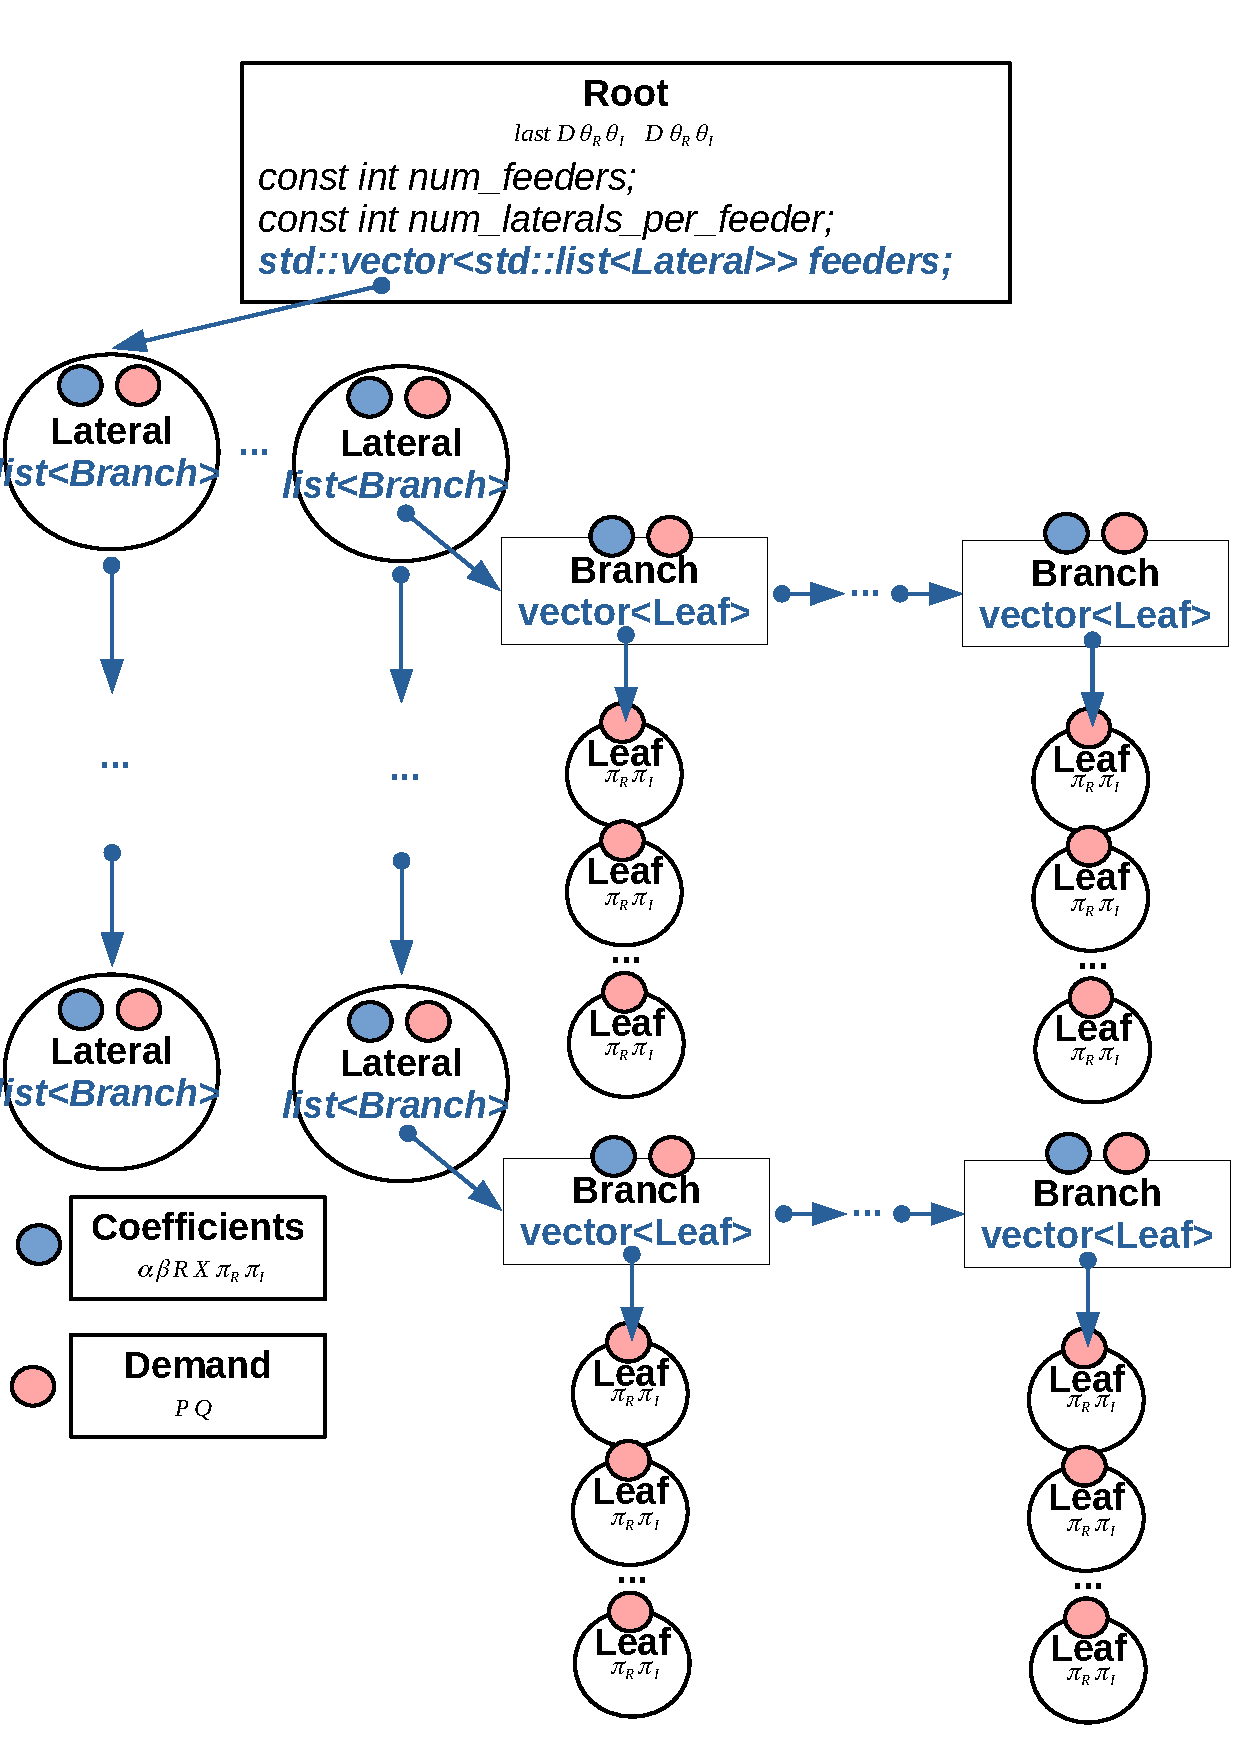
\includegraphics[width=1.0\textwidth]{images/power_scheme.pdf}
\caption{The Power benchmark.}
\label{fig:power_benchmark}
\end{figure}

\paragraph{treeadd} The treeadd benchmark is a very small and simple one. It does a recursive reduction on a pointer-linked binary tree. To create a workload the reduction is done repetitively inside the loop.   

\paragraph{mst} Minimum Spanning Tree (MST) benchmark does a MST weight computation of a complete graph. Computation is approximate and the algorithm looks like it might finish with incorrect result. Nevertheless, the benchmark can be used for the purpose of computational workload. Graph is represented as a linked list of vertices. Every node in the list has a hash table of incident edges. Graph is complete: each vertex is connected to all other vertices in the graph (except itself). Algorithm repeatedly traverses the list of vertices and gradually accumulates the MST weight. On every traversal algorithm picks the node in the list to use as an input for the next traversal. In that sense, there is a cross iteration/traversal dependency. The code below summarises the benchmark.\newline\null
\begin{minipage}[t]{\linewidth}
\begin{lstlisting}[caption={The main algorithm of mst benchmark.},label={lst:mst_code},language=C]
vertex = list;
list = list->next;
while (num_vertices) {
    ret = traverse_vertex_list(vertex, list);
    mst_weight += ret.distance; // accumulate the final result
    vertex = ret.vertex; // next vertex to measure the distance against
    num_vertices--;
}
return mst_weight;
\end{lstlisting}
\end{minipage}

\paragraph{tsp} Travelling Salesman Problem (TSP). The benchmark generates a set of dots scattered on a 2D plane. Dots represent cities and are specified by their (x,y) coordinates. The TSP problem is to visit all the cities and return to the city of origin having passed the minimal distance. In other words, the algorithm returns a cycled sequence of cities, where proximity of elements in the sequence in terms of order means their spatial proximity on the 2D plane.\newline\null
\quad The algorithm’s work resembles that of an insertion sort. The sequence is divided into 2 parts. Ordered part and unordered part. At first, ordered part consists of just 1 element. On every iteration the algorithm takes the next element out of unordered part, finds it a pairing element inside the ordered part (with the minimal distance between them) and inserts the element into the ordered subsequence next to its pair. At the end we get the sequence with the property that closest dots stand the closest in the sequence.\newline\null
\quad The benchmark is based on a binary tree being transformed into doubly linked list. Every node of the tree represents a city located on 2D plane with randomly generated (x,y) coordinates. The build\_tree() method is written in a way to generate a uniform distribution of dots on the plane.







\chapter{Related Work}
\label{related_work}
\quad The topics of parallel computing, parallel software development, and software parallelization have a long and rich history. Historically parallel computers were programmed for doing various scientific simulations, particularly in the natural and engineering sciences. The limits of CPU frequency scaling and power consumption that came in 2004 brought parallel computing to the area of desktop computers and general-purpose applications. Unfortunately, the legacy software did not adapt to these changes transparently and the field of software parallelization came to the spotlight. Software parallelization can be done in a multitude of ways and methods.\newline\null
\quad Section \ref{related_work_autopar} describes a well-known withing the High-Performance Computing (HPC) community field of automatic parallelization. Automatically parallelilizing compilers are largely limited to embarassingly parallel scientific C and Fortran codes. To exploit the potential of upcoming multi-cores, and various heterogeneous systems it will be necessary to extend the scope of automatic parallelization to a broader class of programs containing more complex pointer-based code and finding coarse-grain parallelism. Compilers cannot make such decisions in general as they cannot infer the higher-level semantics of the program. Sections \ref{related_work_ml}, \ref{related_work_dcp}, \ref{related_work_as_and_pp} overview the research studying alternative parallelization strategies. Section \ref{related_work_ml} describes machine learning based methods. Due to the inherent statistical errors of these methods the latter are relatively new to the area of software parallelization, where the program correctness is paramount. The DCP problem has been introduced in Section \ref{background_dcp_problem}. Section \ref{related_work_dcp} provides a literature review on the subject. Lastly, Section \ref{related_work_as_and_pp} provides some references to works addressing the automatic recognition of parallel algorithmic skeletons and higher-level parallelizing program transformations. Unfortunately, these problems are very challenging and not solved yet. Higher-level methods work in a manual or semi-automatic way requiring a programmer to double-check and approve or manually conduct the proposed transformation.
\section{Automatic parallelization in compilers}
\label{related_work_autopar}
\quad There is a large body of work on automatic and semi-automatic parallelization of sequential legacy code \cite{6813266}, \cite{article12345}, \cite{Bacon:1994:CTH:197405.197406}, \cite{Kennedy:2001:OCM:502981}. Years have been spent building various compiler infrastructures for research on parallelizing \cite{Kennedy:2001:OCM:502981} and optimizing \cite{Muchnick:1998:ACD:286076} compilers, e.g., SUIF (Stanford University Intermediate Format) compiler \cite{546613},\cite{10.5555/891422},\cite{suif_compiler}, Polaris \cite{polaris}, \cite{10.1109/M-PDT.1994.329796} and LLVM (Low-Level Virtual Machine) \cite{llvm-compiler-infrastructure},\cite{Lattner:2004:LCF:977395.977673}. Industry has its own well-known and well-established parallelizing compilers like Intel C/C++ Compiler (ICC) \cite{icc-compiler} or GNU Compiler Collection (GCC) project.\newline\null
\quad It is well understood how to parallelize scientific C and Fortran code with perfectly nested loops that operate over flat arrays \cite{97902}, or even non-perfectly nested ones \cite{10.1145/263699.263719}. Furthermore, there are works on how to parallelize sequential loops across procedure boundaries \cite{10.1145/125826.126055},\cite{10.5555/645671.665383}, or with some prior enabling transformations like array privatization \cite{10.1145/158511.158515}. These works, however, focus on loops over arrays. Some research efforts deal with larger code structures
\cite{1299188}. Decoupled software pipelining is a compilation technique to automatically recognize and extract thread-level parallelism from program loops by splitting the instructions of those loops into multiple smaller loops (pipeline stages) that execute in independent threads, and inserting dependence communication where necessary between these threads so that they remain synchronized \cite{1540952}, \cite{10.1145/1400112.1400113}. Software pipelining might require code duplication and eventually lead to a code bloat that, if it is too large, can increase pressure on the cache memory and affect execution speed via a decrease in cache performance. Nevertheless, for loops with large trip counts on architectures with enough instruction level parallelism, the technique easily performs well enough to be worth any increase in code size.\newline\null
\quad Despite all the research efforts automatic parallelization still remains largely limited to sequential scientific codes, where DOALL type loops operate over flat arrays with boundaries known at compile-time. There is a range of reasons that complicate the applicability of automatic parallelization techniques to a wider areas. Dependence analysis is hard for code that uses indirect addressing, pointers, recursion, or indirect function calls because it is difficult to detect such dependencies at compile time. Loops often have statically unknown number of iterations. Accesses to global resources might create race conditions and are difficult to coordinate in terms of memory allocation, I/O, and shared variables. Irregular algorithms that use input-dependent indirection interfere with compile-time analysis and optimization. All enumerated complications are very typical to the real world code. As we demonstrate in Section \ref{backgrnd_challenges_automatic} all above problems can even materialize on a relatively simple and highly parallel suite of NASA Parallel Benchmarks (NPB) \cite{nasa-parallel-benchmarks}.\newline\null
\quad Speculative multithreading or thread-level speculation (TLS) techniques provide a workaround research direction to tackle the limitations of static program analysis. TLS techniques enable parallel execution of sequential applications on a multiprocessor by extracting speculative threads from serial code and submitting them for execution in parallel. At all times, there is at least one safe thread. While speculative threads venture into unsafe program sections, the safe thread executes code non-speculatively. Such techniques speculate the non-existence of dependencies \cite{10.1145/291069.291020} and speculative threads run under some assumptions on the values of input data. Should these assumptions prove wrong, then the state of speculative thread should be discarded. TLS is aware of the order in which such program sections would run in a single-threaded execution. Usually in TLS systems threads are assigned numbers, where the lowest one corresponds to the safe thread. As threads execute, the hardware checks for cross-thread dependence violations. For example, if a thread reads a variable and, later on, another thread with a lower number writes it, a true dependence has been violated. In this case, the offending reader thread is squashed and restarted on the fly. As speculative threads execute, they buffer all their memory state updates into some intermediate structures. If a thread is squashed, the buffer is flushed and all its memory state updates are discarded. If, instead, all the thread’s predecessors complete successfully, the thread becomes safe and it can commit its buffer into the main memory. If all assumptions prove to be correct the program can complete in a shorter time provided there were available hardware resources to schedule the threads efficiently.\newline\null
\quad TLS methods have their own limitations. First, they require a significant hardware support for handling thread contexts, and detecting dependence violations in the memory subsystem \cite{10.1145/1122971.1122997},\cite{10.5555/822079.822712}]. It is possible to implement these mechanisms in software, but then it might incur a significant amount of running time overhead, which would overwhelm any potential performance benefits from speculative-thread parallelism. Overall, speculative parallelization targets the inner program loops \cite{4147670}, \cite{10.1145/1150019.1136512}, \cite{10.1145/1122971.1122997} and cannot handle coarse-grain parallelism, especially if the loops contain I/O or other system calls \cite{10.1016/j.parco.2010.05.006}.\newline\null
.
\section{Machine learning in compilers}
\label{related_work_ml}
\quad Correctness is the most important property of the code. Although important, the running time or any other type of code performance characteristic is not always vitally critical. As all machine learning based techniques have always been characterized by their inherent and ineradicable errors \cite{James:2013:ISL:2517747}, the field of compilers has never been the primary target for these methods. Nonetheless, these techniques have found their application to some problems within the field.\newline\null
\textit{ML in Compiler Optimization.}
Usually, machine learning based methods target problems, where a misprediction will only lead to a hampered performance and not a functional failure. For example, machine learning based methods have been used for finding the most optimal compiler optimization parameters like predicting the optimal loop unroll factor \cite{4907653,1402082} or determining whether or not a function should be inlined \cite{Zhao2003ToIO,1559966}. These works are supervised classification problems and they target a fixed set of compiler options, by representing the optimization problem as a multi-class classification problem where each compiler option is a class. Recent works try to do scheduling and optimization of parallel programs for heterogeneous multi-cores. For example, Hayashi \emph{et al.}~\cite{Hayashi:2015:MPH:2807426.2807429} extracts various program features during compilation for use in a supervised learning prediction model aiming at the optimality of CPU vs. GPU selection. Evolutionary algorithms like generic search are often used to explore a large design space. Prior works~\cite{Almagor:2004:FEC:997163.997196,Cooper:2005:AAC:1065910.1065921,Ashouri:2017:MMC:3132652.3124452} have used evolutionary algorithms to solve the phase ordering problem (i.e.\ in which order a set of compiler transformations should be applied).\newline\null
\textit{Machine Learning and Parallelization.}
The application of machine learning based methods to the problem of software parallelization has not yet found a widespread practical utility. Mispredictions regarding the code parallelizability can lead to a broken dependency property and thus incorrect program execution. Nonetheless, there have already been works on predicting loop parallelizability, like the approach of Fried \emph{et al.}~\cite{fried_ea:2013:icmla}. Fried \emph{et al.} train a supervised learning algorithm on code hand-annotated with OpenMP parallelization directives to create a loop parallelizability predictor. These directives approximate the parallelization that might be produced by a human expert. Fried \emph{et al.}~focus on the comparative performance of different ML algorithms and studies the predictive performance that can be achieved on the problem and does not produce any practical application.\newline\null
\section{Discovery: data structure recognition}
\label{related_work_dcp}
\quad The idea of automatic discovery of higher-level entities in programs is not a new one. This discovery problem is closely interlinked and entangled with alias analysis techniques \cite{Muchnick:1998:ACD:286076} like points-to analysis \cite{Emami:1994:CIP:178243.178264}. The Points-to analysis is a variation of data flow analysis techniques. The final output is the sets of pairs of the form (\textit{p}, \textit{x}) (pointer variable \textit{p} points to a stack-allocated variable \textit{x}). These techniques are aimed at getting aliasing information regarding stack-allocated pointers.\newline\null
\quad The problem of understanding heap-directed pointers and heap-allocated linked data structures these pointers might point to is addressed with a family of static analysis techniques collectively known as shape analysis. Shape analysis techniques can be used to verify properties of dynamically allocated data structures in compile time. These are among the oldest and most well-known techniques. Three-valued logic \cite{Sagiv:1999:PSA:292540.292552}\cite{Wilhelm:2000:SA:647476.760384} can be used as an example. The technique proposes the construction of a mathematical model consisting of logical predicate expressions. The latter correspond to certain pointer operating imperative language program statements. An abstract interpretation of these statements leads to the construction of sets of shape graphs at various program points. Shape graphs approximate the possible states of heap-allocated linked data structures and answer the questions such as node reachability, data structure disjointness, cyclicity, etc. The major limitation of these simplified mathematical models is the lack of precision high level of abstraction leads to. The problem of precise shape analysis is provably undecidable.\newline\null
\quad The work of \cite{Ghiya:1996:TDC:237721.237724} proposes a simplified and hence more practical implementation of shape analysis. Authors propose to use direction \textit{D} and interference \textit{I} matrices instead of complex mathematical models to derive shape information on heap-allocated data structures. The entry of direction matrix \textit{D[p,q]} says if there exists a path from a node referred to by \textit{p} to a node referred to by q. In other words, if we can enter a path within the data structure through \textit{p} and exit through \textit{q}. The entry of interference matrix \textit{I[p,q]} says if the paths started from \textit{p} and \textit{q} are going to intersect at some point. Authors implement their technique withing McCAT compiler, which uses SIMPLE intermediate representation with a total of 8 statements (\textit{malloc()}, pointer assignments \textit{p=q}, structure updates \textit{p-$>$next=q}), which are capable of changing \textit{D} and \textit{I} matrices. Statements generate and kill entries in matrices. Moreover, they are capable of changing \textit{Shape} attributes of pointers. The technique has been assessed on various benchmarks (bintree, xref, chomp, assembler, loader, sparse, etc.) from the era before the standard benchmark suites became available. The technique mostly reported shapes as \textit{Trees} (be it a binary tree or a linked-list) or sometimes as \textit{DAGs} or \textit{Cycles} but with higher error rates in these last cases. The latter shows that the technique is imprecise and conservative.\newline\null
\quad One of the more recent techniques designed and developed by Ginsbach et al. is based on the pattern matching on LLVM IR level. The main idea is to specify computational idioms to be recognized in a domain-specific constraint-based programming language CAnDL \cite{Ginsbach:2018:CDS:3178372.3179515}. Constraints are specified over LLVM IR entities such as instructions, basic blocks, functions, etc. The CAnDL language allows rapid prototyping of new compiler optimizations based on pattern recognition and its substitution with optimized versions of matched idioms. The language and its relatively fast backtracking constraint solver are capable of recognizing not only simple arithmetic idioms (thus performing different peephole optimizations), but more complex computations like general reductions and histograms \cite{Ginsbach:2017:DEG:3049832.3049862}, vector products in graphics shaders \cite{Ginsbach:2018:AML:3296957.3173182}, sparse and dense linear algebra computations and stencils \cite{Ginsbach:2018:AML:3296957.3173182}. Having recognized these computational idioms the work \cite{Ginsbach:2018:AML:3296957.3173182} replaces them with a code for various heterogeneous APIs (MKL, libSPMV, Halide, clBLAS, CLBlast, Lift) and compares the resulting performance demonstrating an improvement over sequential versions and matching performance to hand-written parallel versions. The technique has been deployed on the sequential C versions of SNU NPB, the C versions of Parboil, and the OpenMP C/C++ versions of Rodinia demonstrating improved detection capabilities over the state-of-the-art techniques.\newline\null
\quad The other principally different technique has been recently proposed by Changhee Jung and Nathan Clark \cite{1669122}. The authors developed a Data-structure Detection Tool (DDT) based on the LLVM framework. The tool instruments load, store, and call instructions within program binaries and gathers dynamic traces for sample inputs. The traces are used to recreate a memory allocation graph for program data structures. Call graphs are used to identify interface functions interacting with the built memory graph. DDT traces memory graph properties (number of nodes, edges, etc.) before and after interface function calls into another Daikon tool to compute dynamic invariants (the number of nodes in a memory graph decreases by 1 after every \textit(delete()) interface method call, etc.). In the end, manually constructed decision tree is used to probabilistically match observed behavioral patterns against known data structure invariant properties. The technique has been deployed to recognize data structure implementations within standard libraries like STL, Apache (STDCXX), Borland (STLport), GLib, Trimaran achieving almost perfect recognition accuracy. Moreover, the technique has been able to recognize linked lists in Em3d and Bh Olden benchmarks, along with red-black trees implementing vectors in the Xalancbmk benchmark.\newline\null
\quad There has recently been other published works on the application of dynamic techniques to the problem of dynamic data structure recognition \cite{Rupprecht:2017:DID:3155562.3155607}\cite{Haller:2016:SDS:2938006.2938029}. The technique used in the DDT tool \cite{1669122} makes an assumption, that all modifications and interactions with memory graphs representing data structures happen through a set of interface functions. That is not true when we deal with aggressively optimizing compilers, which may eliminate some code or inline some functions. The MemPick tool \cite{Haller:2016:SDS:2938006.2938029} searches data structures directly on a built dynamic memory graph by analyzing its shape. The graph is built with the help of the Intel Pin binary instrumentation tool during quiescent periods when pointer operations are absent. DSIbin tool \cite{Rupprecht:2017:DID:3155562.3155607} operates with the source code rather than program binaries. Instead of memory points-to graphs, it uses strands as primitives, which abstract such entities as singly-linked lists.\newline\null
\quad The work of Dekker \cite{Dekker:1994:ADS:3107859.3107876} addresses the software design recovery problem in a completely different way. Contrary to the approaches described above, which operate on the IR and dynamic instruction stream levels, the work of Dekker operates at the level of an abstract syntax tree. Dekker's tool tries to compact the tree down to recognizable syntactic patterns by transforming it under a special grammar.
\section{Discovery: algorithmic skeletons and parallelism patterns}
\label{related_work_as_and_pp}
\quad Parallelizing sequential applications is a challenging and labour-intensive task, which requires of a programmer to possess a deep expertise in various fields. Parallelization can be done in numerous ways, due to many different ways in which an application can be parallelized and a large number of various programming models that can be used. The concept of algorithmic skeletons (parallelism patterns) (see Section \ref{background_skeletons}) has been proposed to alleviate the challenging task and provide a programmer with a portable human-friendly model of parallel computations. There is a vast array of various frameworks and libraries that implement the concept. They vary by the programming language they target, distribution library used to implement parallel/distributed computations internally (like MPI \cite{mpi}, OpenMP \cite{openmp_specs}, etc.), the sets of supported skeletons, and the allowed level and way of skeleton nesting, i.e composing more complex patterns of the basic ones; these include: RPL \cite{7445342}; Feldspar [4]; FastFlow [2]; Microsoft’s Pattern Parallel Library \cite{microsoft-ppl}; and Intel’s Threading Building Blocks (TBB) library \cite{intel-tbb}.\newline\null
\quad Although, the libraries of parallelism patterns alleviate the process of parallel software development, their use still requires a manual effort. Before using a particular library, a programmer has to invest time and efforts into learning its target use and limitations. Furthermore, discovering places in
sequential code where parallel patterns might be introduced is
still highly non-trivial, often requiring expert manual analysis and profiling. There is a number of works addressing the task of automatic discovery of parallel patterns.\newline\null
\quad The work \cite{skeletons-static} proposes a static approach and develops Parallel Pattern Analyzer Tool (PPAT) capable of analyzing sequential C++ code statically in order to detect and annotate parallel patterns. The tool takes advantage of a Clang library to generate an Abstract Syntax Tree (AST). Then, it walks through it finding AST loop candidates to be analyzed for possible parallel patterns. For every loop the tool checks a set of constraints specific for every target pattern. For example, for a loop in order to be a parallel pipeline, it must not write any global variables, pass no feedback between separate loop body stages, and there must be at least two stages to split the loop into. The tool uses a set of heuristics to determine the size of stages. For farm pattern, the tool checks that loop body has no RAW dependencies, no break statements, and writes no global variables. Authors evaluate the effectiveness and correctness of their approach using NAS \cite{nasa-parallel-benchmarks} and Rodinia benchmark suites by comparing automatically detected patterns against the manual analysis. Authors observe that the pattern detection quality of PPAT is close to that performed by a human expert. Then, the authors move on manually parallelizing detected patterns demonstrating final performance comparable to expertly parallelized benchmark versions. The experimental evaluation demonstrates that PPAT is able to obtain similar performance results as the “handmade” parallel versions of the benchmark suites tested. Therefore, reducing the human effort in transforming sequential codes into parallel.\newline\null
\quad Some works take advantage of functional languages. For instance, István Bozó et al. \cite{10.1145/2633448.2633453} develop a tool that detects parallel patterns in applications written in Erlang. Compared to other languages, Erlang
features make the detection process much simpler. Nonetheless, the tool requires profiling techniques in order to decide which pattern suits best for a concrete problem.\newline\null
\quad The work \cite{roberto-lozano-skeletons} aims to highlight to a programmer code fragments, which could be replaced by calls to known parallel pattern library abstractions of map, reduce and their compositions in a legacy Pthreaded C/C++ code. The underlying technique is based on the analysis of dynamic data flow graphs (DDFGs) obtained during execution of programs and thus is language-agnostic. The analysis uses constraint-based pattern matching to identify constrained DDFG subgraphs characteristic to the well-established parallel patterns while employing heuristics which trade analysis time against completeness making the approach scalable. The tool and methodology demonstrate an excellent effectiveness and accuracy on Starbench benchmarks by finding 36 out of the expected 42 instances of parallel patterns with a high accuracy (reporting actual patterns in 98\% of the cases). Authors re-express the found patterns via a parallel pattern library, making code freely portable across CPU/GPU systems and performing competitively with hand-tuned implementations at zero additional effort.\newline\null
\quad There are also hybrid methods of parallel pattern discovery. The work \cite{9092377} employs both static and dynamic trace-based analysis, together with hotspot detection. First, using running time profiling the methodology obtains a list of hotspot loop candidates, which pass though a static analysis, leveraging the existing Pattern Analyzer Tool PPAT \cite{skeletons-static}. Independently from the static analysis, candidate loops are also passed through a new dynamic trace-based pattern detection mechanism. Finally, the user checks manually that the candidate detected patterns (from either analysis) are indeed applicable. The mechanism is evaluated on a number representative benchmarks, demonstrating good accuracy, precision and recall scores for map and reduce algorithmic skeletons. The scores are compared against the manual analysis.\newline\null
\quad As the sequential code gives the cleanest starting point for the introduction of parallel patterns, the work \cite{} studies how parallel legacy C/C++ pthreaded codes could be converted back to sequential version and ultimately restored to a modern parallel pattern based equivalent form. This work studies the specifics of parallel legacy pthreaded codes and proposes a novel methodology to accomplish the task. The restoration is conducted through a systematic application of a number of identified program transformations. Authors design and define a set of restorative transformations common to many legacy pthreaded codes. The aim of these transformations is to (i) eliminate Pthread operations from legacy C/C++ programs; (ii) perform code repair, fixing any bugs introduced in (i); and, (iii) reshape code in preparation for parallel pattern introduction. The work targets only farm and pipeline patterns. The transformations presented in the work are intended as manual transformations. The implementation of these refactorings into a semi-automatic tool is envisaged as the future work. Authors use Intel TBB library to evaluate these transformations on a set of benchmarks and demonstrate that the removal of parallelism allows to manually derive structured parallel code that is comparable to the original legacy-parallel version in terms of performance, while being more portable, adaptive, and maintainable. Additionally authors record improvements in terms of cyclomatic complexity \cite{} and Lines Of Code (LOC) metric.



\chapter{Software Parallelization Assistant}
\label{assistant}
\section{Introduction}

% problem: the need for manual parallelization, auto-parallelisation does not deliver desired performance improvements

\quad Parallel hardware is ubiquitous through the entire spectrum of computing systems, from low-end embedded devices to high-end supercomputers.
%
Yet, most of the existing software is written in a sequential fashion.
%
Despite decades of intensive research in automatic software
parallelization~\cite{6813266}, fully exploiting the potential of modern parallel hardware still requires a significant manual effort.
%
Given the difficulty of the obstacles faced by automatic parallelization today, we do not expect that programmers will be liberated from performing manual parallelization in the near future~\cite{Larsen:2012:PML:2410141.2410600}.

% solution: parallelisation assistant

This chapter introduces a novel parallelization assistant that aids a programmer in the process of parallelizing a program in the frequent case where automatic approaches fail.
%
The assistant reduces the manual effort in this process by presenting a programmer with a ranking of program loops that are most likely to 1) require little or no effort for successful parallelization and 2) improve the program's performance when parallelized.
%
Thus, it improves over the traditional, profile-guided process by also taking into account the \emph{probability} of potential parallelization for each of the profiled loops.

% how?

At the core of our parallelization assistant resides a novel machine-learning (ML) model of loop parallelizability.
%
Loops are compelling candidates for parallelization, as they are naturally decomposable and tend to capture most of the execution time in a program.
%
Furthermore, focusing on loops allows the model to leverage a large amount of specific analyses available in modern compilers, such as generalized iterator recognition~\cite{Manilov:2018:GPI:3178372.3179511} and loop dependence analysis~\cite{Jensen:2017:ILD:3132652.3095754}.
%
The model encodes the results of these analyses together with basic properties of the loops as machine learning \textit{features}.

The loop parallelizability model is trained, validated, and tested on 1415 loops
from the SNU NAS Parallel Benchmarks (SNU
NPB)~\cite{Seo:2011:PCN:2357490.2358063}.
%
The loops are labelled using a combination of expert OpenMP~\cite{Dagum:1998:OIA:615255.615542}
annotations and optimization reports from Intel \cpp{} Compiler (ICC), a
production-quality parallelizing compiler.
%
The model is evaluated on multiple machine learning algorithms, including tree-based methods, support vector machines, and neural networks.
%
The evaluation shows that -- despite the limited size of the data set -- using
support vector machines allows the model to achieve a prediction accuracy higher than 90\%.
%
% Note: the "detected parallelism increase" is 945/995 - 812/995 = 0.1336683417.
%
The model improves over the ICC Compiler across the sequential C version of the SNU NPB suite by detecting 13\% more parallel loops. Albeit this improvement comes at the cost of introducing \textit{false positives}, where non-parallelizable loops are misclassified as parallelizable. However, the false positive rate in our evaluation is as low as 6.5\%. We feel this is acceptable, as our parallelization assistant does not automatically restructure code but leaves the parallelization decision in the hands of the programmers.
%\todo{(FIXME: taken from~Figure~\ref{fig:accuracy_loocv}, double-check these numbers)}

% TODO: mention that we use standard techniques for feature extraction,
% hyper-parameter tuning, and cross-validation?

The parallelization assistant combines inference on the parallelizability model
with traditional profiling to rank higher those loops with a high probability of being parallelizable and impacting the program performance.
%
An evaluation on eight programs from the SNU NPB suite shows that
the program performance tends to improve faster as loops are parallelized in the ranking order suggested by our parallelization assistant compared to a traditional order based on profiling only.
%
On average, following the order suggested by the assistant reduces by approximately 20\% the number of lines of code a programmer has to examine manually to parallelize SNU NPB to its expert-level speedup.
%
Given the high level of effort involved in manual analysis, such a reduction
can translate into substantial development cost savings.

\subsection{Motivating example}\label{motivating_example}
\quad Consider the sequential C implementation of the \textit{Conjugate Gradient (CG)}
benchmark from the SNU NPB suite.
%
Table~\ref{tab:ranking} shows the top three CG loops as ranked by the Intel
Profiler (based on their execution time) and by our parallelization
assistant (additionally taking into account their parallelizability).
%
Both rankings include the same loops, but, crucially, the loops are \textbf{ranked in a different order}.
\begin{table}
  \begin{minipage}{\columnwidth}
  \begin{center}
    \begin{tabu}{c|c|cc}
      \hline
      \rowfont{\bfseries}
      \multirow{2}{*}{Ranking} & Profiler & \multicolumn{2}{c}{Assistant} \\ \cline{2-4}
      \rowfont{\bfseries}
      & loop & loop & parallelizability\\\hline
      1 & \texttt{cg.c:326} & \textbf{\texttt{cg.c:509}} & 85\%\\
      2 & \texttt{cg.c:484} & \texttt{cg.c:326} & 29\%\\
      3 & \textbf{\texttt{cg.c:509}} & \texttt{cg.c:484} & 8\%\\\hline
    \end{tabu}
    \caption{Comparison of the profiler and assistant rankings for the CG benchmark loops (limited to the top three loops).}
    \label{tab:ranking}
  \end{center}
  \end{minipage}
\end{table}%
Following the profiler ranking (second column in Table~\ref{tab:ranking}), a
parallelization expert would concentrate on analyzing the loop \texttt{cg.c:326}
first.
%
% Note: the 100 lines of code are counted using 'cloc code/cg-326.c'.
%
Analyzing this loop turns out to be costly (it consists of 100+ lines of code)
and unfruitful (it is actually not parallelizable due to inter-iteration
dependencies and side effects, see Listing~\ref{lst:main_iter}).
%
This analysis would be followed by an equally unfruitful analysis of
loop \texttt{cg.c:484}.

In contrast, our parallelization assistant (two last columns in
Table~\ref{tab:ranking}) ranks the loop \textbf{\texttt{cg.c:509}} before
loops \texttt{cg.c:326} and \texttt{cg.c:484}, as it finds that the former has a
significantly higher probability of being parallelizable (see last column in
Table~\ref{tab:ranking}).
%
Following the assistant's ranking, a parallelization expert would thus
concentrate on analyzing the loop \textbf{\texttt{cg.c:509}} first.
%
Analyzing this loop is inexpensive (it consists of only six lines of code, see
Listing~\ref{lst:reduction}) and fruitful: its parallelization speeds up CG by a
factor of~2.8, which is~70\% of the speedup obtained by parallelizing the entire
benchmark.
%
Hence, following the ranking proposed by our assistant, a parallelization expert
can achieve most of the available speedup in CG in a fraction of the time
required by a traditional profile-guided parallelization process.
\begin{figure}[t]
\begin{lstlisting}[caption={\texttt{cg.c:326}. Longest running loop in CG. The loop cannot be parallelized due to
inter-iteration dependences and side effects caused by system calls.},label={lst:main_iter},language=C]
for (it = 1; it <= NITER; it++) {
  ...
  if (timeron) timer_start(T_conj_grad);
  conj_grad(colidx,rowstr,x,z,a,p,q,r,&rnorm);
  if (timeron) timer_stop(T_conj_grad);
  ...
  printf("    %5d       %20.14E%20.13f\n", it, rnorm, zeta);
  ...
}
\end{lstlisting}
\begin{lstlisting}[caption={\textbf{\texttt{cg.c:509}}. Longest running loop in CG among those \emph{that can be parallelized}.},label={lst:reduction},language=C]
for (j = 0; j < lastrow-firstrow+1; j++) {
  suml = 0.0;
  for (k = rowstr[j]; k < rowstr[j+1]; k++)
    suml = suml + a[k]*p[colidx[k]];
  q[j] = suml;
}
\end{lstlisting}
\end{figure}
\subsection{Contributions}
\quad In summary, this project makes the following contributions:
%
\begin{itemize}
\renewcommand\labelitemi{$\vartriangleright$}
\renewcommand\labelitemii{$\bullet$}
\item We introduce a machine learning model, which can be used to predict the probability with which sequential C loops can be parallelized (Sections~\ref{predicting_parallel_loops} and~\ref{ml_predictive_performance});
\item we integrate profiling of execution time with our novel ML model into a parallelization assistant, which guides the user through a ranked list of loops for parallelization (Section~\ref{practical_applications}); and
\item we demonstrate that our tool and methodology increase programmer productivity by identifying parallel loop candidates better than existing state-of-the-art approaches (Section~\ref{evaluation}).
%Designed an ML based model of loop parallelisability quantifying the latter %(Section~\ref{predicting_parallel_loops}) and ranking program loops
%    \begin{itemize}
%    \item Devised loop parallelisability metrics (ML loop features)
%    \item Prepared a labelled training set with classification labels
%    derived from SNU NPB OpenMP \textit{\#pragmas} as well as Intel Compiler %optimisation reports
%    \item Set and tuned an ML train/test methodology
%    \end{itemize}
%\item Conducted a thorough evaluation of the model demonstrating prediction %accuracy
%  higher than 90\% on~\numprint{\totalLoops{}}~loops from the SNU NAS Parallel
%  Benchmarks (\textcolor{red}{Section~4})
%\item Integrated the model into a parallelisation assistant scheme that %automatically ranks promising loops by combining profiling information and %model inference (\textcolor{red}{Section~5})
%    \begin{itemize}
%    \item Demonstrated improved parallelism discovery capabilities of %assistant in comparison with Intel Compiler 
%    \end{itemize}
%\item Deployment of the assistant on SNU NAS Parallel Benchmarks demonstrating %its potential to ease parallelisation process and converge to the maximum %attainable performance faster
%    \begin{itemize}
%    \item Conducted a performance study of SNU NPB with the state-of-the-art %Intel Compiler
%    \item Parallelisied SNU NPB following profiler and assistant suggested %loop orders and plotted performance convergense curves
%    \end{itemize}
%
% a demonstration of the assistant's potential to reduce the manual effort
%  involved in the traditional profile-guided parallelisation methodology
%  (\textcolor{red}{Section~6}).
\end{itemize}
%% 1) We show that it is possible to learn loop
%% have successfully learnt the parallelisability property o
%% 2) We conduct a study of Intel Compiler's behaviour on SNU NPB benchmarks. We summarise the exact optimizations applied (see section [?]), classify missed parallelisation opportunities (see section [?]) and
%% \subsection{Overview}

%% \subsection{Paper structure}
%% \quad The most substantial part of this work was aimed at the creation of machine learning (ML) based model, capable of accurate prediction of loop parallelisability property. Section \ref{predicting_parallel_loops} describes all the details of machine learning part including the features we chose and the exact training/testing methodology we used. But even close to perfect prediction accuracy is not enough, if we cannot find a real practical application to utilise our predictor. Section \ref{practical_applications} proposes 2 complementary schemes we might integrate our predictor into. The first scheme helps Intel ICC compiler to discover additional parallelism. The second scheme is basically software manual parallelisation assistant working with a program profile and directing human efforts at the most likely to be parallelisible (and profitable as well) loops. Section \ref{evaluation} presents a quantitative report on our work.  
\section{Predicting parallel loops}
\label{predicting_parallel_loops}
\quad We approach the prediction of parallel loops as a \emph{supervised probabilistic machine learning classification problem}. Based on sequential reference applications and their manually parallelized counterparts as well as Intel's parallelizing C/C++ compiler, we create a data set of parallelizable and non-parallelizable loops. We extract loop features and use the data set to train a machine learning model, which links feature vectors describing the loops with their observed parallelizability. We then use the trained model as a probabilistic predictor: for each new loop we determine its feature vector and then predict the probability of the loop being parallelizable \cite{Niculescu-Mizil:2005:PGP:1102351.1102430}. For naturally probabilistic models like trees we directly use the computed classification probabilities (fraction of parallelizable training samples in the leaf node). For the support vector machines classifier, we use Platt scaling to derive the probabilities.

In this section we introduce the parallelizability model, whereas Section~\ref{ml_predictive_performance} presents a standard ML performance assessment including accuracy, precision and recall scores. Descriptions and definitions of the machine learning techniques we use can be found in \cite{James:2013:ISL:2517747}. We used the \textit{scikit-learn} library~\cite{scikit-learn} for all ML related tasks.

\subsection{Loop analysis \& feature extraction}
\label{loop_analysis_and_features}
\quad For the purpose of machine learning, program loops are represented by numerical \textit{feature vectors}. We derive these features using standard compiler analyses operating on the Program Dependence Graph (PDG)~\cite{Ferrante:1987:PDG:24039.24041} of a loop. The PDG is a representation that captures both data and control information and is constructed using dependence analysis~\cite{Kennedy:2001:OCM:502981}. Figure \ref{fig:pdg} shows an example of a PDG for a simple loop, where SCC stands for \emph{Strongly connected component}.
\begin{figure}[ht]
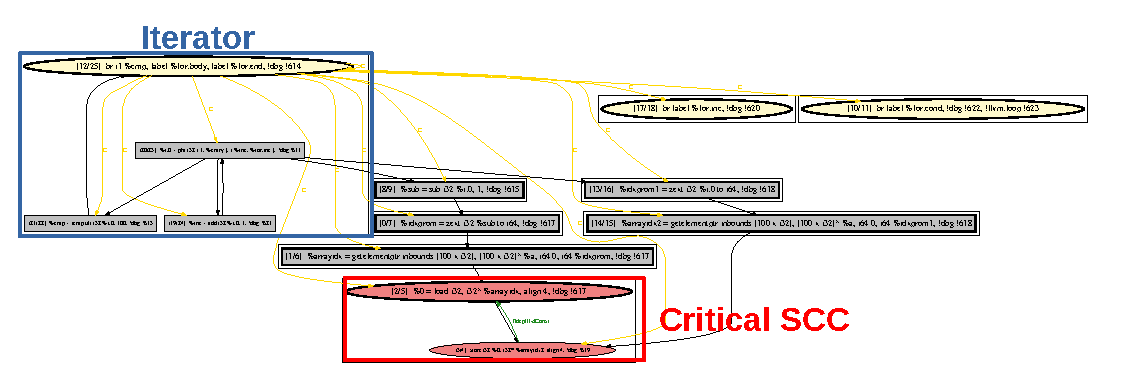
\includegraphics[width=1.0\textwidth]{images/pdg_example.pdf}
\caption{Example of PDG of a simple loop with a cross-iteration dependency.}
\label{fig:pdg}
\end{figure}
We construct the PDG on a program's LLVM IR and apply standard dependence analysis. In addition we use \textit{generalized loop iterator recognition}~\cite{Manilov:2018:GPI:3178372.3179511} to separate \textit{loop iterators} from \textit{loop payloads}. This enables us to define and extract features relating to each of those loop components. In total, we extract a set of 74 static loop features which are based on structural properties of the PDG and the types of instructions constituting it. Table \ref{tab:loop_features} summarizes these features.\newline\null
\quad Our features have simple and intuitive motivations behind them. Loop proportion features are backed up by the fact that larger loops tend to be harder to parallelize. Complex iterators include non-trivial cross-iteration transitions (e.g linked-list update), unknown iteration numbers, etc. Payload SCCs (Strongly Connected Components) introduce cross-iteration dependencies. Cohesion features characterize how tightly components of loops are coupled together in terms of the number of edges between them. Loop dependence features count the number of edges in different loop parts as well as their types. Loop instruction features characterize the loop's instruction mix, assigning more importance to memory reads/writes, calls and branches. Non-inlined function calls usually prevent loop parallelization. Intensive memory work (memory read/write fraction features) complicates parallelization as well.
\begin{table*}[!ht]{\linewidth}
  \tabulinesep=2pt
  \begin{minipage}{\linewidth}
  \begin{center}
    \begin{tabu}{M{3cm}M{3.0cm}M{5.0cm}}
      \hline
      \rowfont{\bfseries}
      Feature groups & Features & Description\\\hline
      \multirow{3}{*}{loop proportion} & absolute size & number of LLVM IR instructions\\%\hline
      & payload fraction & $\text{payload instructions} \, / \, \text{total loop instructions}$\\%\hline
      & proper SCCs number & number of payload SCCs with more than 1 instruction\\\hline
      loop dependencies & \multicolumn{2}{M{11cm}}{number of PDG edges for different dependence classes: read/write order (\emph{true}, \emph{anti}, \emph{output}), dependency type (\emph{register}, \emph{memory}, \emph{control}), other (\emph{cross-iteration}, etc.)}\\\hline
      \multirow{2}{*}{loop cohesion} & iterator/payload & $\frac{\text{edges between iterator}/\text{payload}}{\text{total loop edges}}$\\
        & critical/regular payload & $\frac{\text{edges between critical/regular payload}}{\text{total loop payload edges}}$\\
        \hline
      loop instruction nature & \multicolumn{2}{M{11cm}}{numbers and fractions of different parallelization critical instructions (memory loads and stores, branches, calls, etc.)}\\\hline
      \end{tabu}
  \end{center}
  \caption{Static features used for the characterization of loops.}
  \label{tab:loop_features}
  \end{minipage}
\end{table*}%
\subsection{Feature extraction}
\label{feature_extraction}
\quad To extract all devised loop features from SNU NPB benchmarks and get the train/test data set we developed a tool based on the LLVM compiler infrastructure \cite{llvm-compiler-infrastructure}\cite{Lattner:2004:LCF:977395.977673}. The tool is a set of LLVM function passes working on the SSA-based LLVM IR and can be found on the GitHub \cite{github-ppar-tool}. The tool works by building data, memory and control dependence graphs (DDG, MDG, CDG) and combining them into the final program dependence graph (PDG) \cite{Ferrante:1987:PDG:24039.24041} for all loops found in program functions. Once all graphs are built we run the search of strongly-connected components (SCCs) on them and recognise loop iterators. The final step is to traverse all these graphs computing devised metrics (ML features) and dump all that information into the file to be later fed into scikit-learn based ML scripts.
\subsection{Feature selection}
\label{feature_selection}
\quad The feature engineering task resulted into a quantitative description of program loops being characterised by feature vectors of length 74. To avoid overfitting, we discard irrelevant or redundant features using a pipeline of feature selection methods from the scikit-learn library. First we eliminate features with a low variance score, then we fit a decision tree-based model and select features with importance score above a given threshold. After that we repeatedly run \textit{Recursive Feature Elimination, Cross-Validated (RFECV)} to improve accuracy, precision and recall scores. This yields the final set of features. Table \ref{tab:best_features} presents the 10 highest-ranked features in this set. SNU NPB benchmarks contain a lot of uninlined function calls and it is unsurprising that the amount of call instructions in the payload of a loop ranks the highest. Despite the absence of straightforward intuition behind cohesion metrics, they tend to correlate with parallelization labels well. Loops heavy on memory writes also significantly affect the parallelizability property.
\begin{table}[ht]
  \begin{minipage}{\columnwidth}
  \begin{center}
    \begin{tabu}{lc}
      \hline
      \rowfont{\bfseries}
      \multicolumn{1}{l}{Feature} & \multicolumn{1}{l}{Importance}\\\hline
      payload call fraction & 23.5\\
      iter/payload non-cf cohesion & 18.5\\
      payload mem write fraction & 6.1\\
      loop absolute size & 5.7\\
      critical payload pointer access count & 5.3\\
      payload memory dependence count & 4.0\\
      critical payload non-cf cohesion & 2.9\\
      payload pointer access fraction & 2.7\\
      critical payload total cohesion & 2.6\\\hline
      \end{tabu}
  \end{center}
  \end{minipage}
  \label{tab:best_features}
  \caption{Relative importance of static loop features, ranked by fitting a tree-based ML model.}
\end{table}
\subsection{Model \& hyper-parameter selection}
\label{model_selection}
\quad We evaluate several machine learning classification algorithms in our parallelization assistant, including tree-based methods like decision trees (DT), random forests (RFC) and boosted decision trees (AdaBoost); support vector machines classifiers (SVC) and multi-layer perceptron neural networks (MLP). Section \ref{evaluation_kfold} shows that these models perform similarly with SVC and MLP performing slightly better. For each ML model we use exhaustive hyper-parameter grid search and pick the grid node with the best cross-validation score on the validation set.  The details of all ML pipeline stages are available in our repository \cite{assistant-repo}.
\subsection{Training data \& ML model training}
\label{loop_classification_labels}
\quad In order to train and test our ML model in a supervised way, first we need to provide it with the "right answers" regarding loop parallelizability. In other words we need to prepare a training data set.\newline\null
\quad For training our ML model we use a total of 1415 loops from the SNU NPB benchmark suite. Out of those loops, 210 have been annotated by (external) human experts with parallel OpenMP \textit{pragmas}. We use these annotations as labelled data to indicate parallelizable loops. However, the data is not complete. Human programmers strive to capture only coarse-grain parallelism and do not annotate every parallelizable loop. Hence, we augment the training data with the help of the ICC Compiler, which finds additional parallelizable loops. We combine the results into our training set comprising a total 1415 loops, of which 995 are labelled as parallelizable. Then we use K-fold and Leave-One-Out Cross-Validation (LOOCV) methodologies to train and test our ML models.\newline\null
\quad To extract loop parallelizability labels from the Intel compiler's optimization reports we developed a parser \cite{github-icc-parser}, but the task has presented us with a number of technical challenges. Before ICC can actually parallelize or vectorize a loop, it applies a number of enabling loop transformations such as loop interchange, distribution, tiling, etc. The detailed description of all these transformations can be found in the paper \cite{Bacon:1994:CTH:197405.197406}. Applied to a loop nest, these optimizations might significantly restructure and distribute the parts of a loop across the whole ICC optimization report. Moreover, ICC might parallelize only certain parts of transformed loop. At the end we considered a loop to be parallelizable by the ICC compiler if the latter hasn't found any dependencies and either vectorized or parallelized it. In the case of distributed loops, all parts must be parallelizable for an original loop to be considered as such. For a final correctness we conducted a manual verification on top of automatically extracted results.\newline\null
\quad Table \ref{tab:icc_stats} presents a parsing report, which summarises the number of times ICC applied a certain optimization. The major cells are \textit{parallel} and \textit{icc}, which report the total number of truly parallelizable loops and the number of loops parallelized by ICC. As it can be seen ICC compiler does not exploit all the parallelism available in SNU NPB benchmarks. Section \ref{background_challenges_automatic} presented a study of reasons ICC fails to parallelize certain loops.
\begin{table}
  \begin{minipage}{\columnwidth}
  \begin{center}
    \begin{tabu}{cccccc}
      \hline
      \rowfont{\bfseries}
      \multicolumn{2}{c}{\multirow{2}{*}{Labels}} & \multicolumn{4}{c}{Intel Compiler (ICC)} \\%\hline
      \rowfont{\bfseries}
      & & \multicolumn{2}{c}{Optimisation} & \multicolumn{2}{c}{Parallelisation}\\\hline
      loop & ranking & loop & ranking & parallel \\\hline
      \textbf{total loops} & \textbf{1415} & distrs & 34 & parallel & 653\\
      \textbf{parallel} & \textbf{995} & fusions & 214 & vector & 737\\
      \textbf{icc} & \textbf{812} & collapses & 58 & parallel deps & 535\\
      \textbf{openmp} & \textbf{210} & tilings & 27 & vector deps & 266\\\hline
    \end{tabu}
  \end{center}
  \end{minipage}
  \caption{Report on loop classification labels derived out of expertly added OpenMP annotations of SNU NPB benchmarks and ICC optimization reports. Out of 995 parallelizable loops ICC discovered and parallelized 812.}
  \label{tab:icc_stats}
\end{table}
\section{ML predictive performance}
\label{ml_predictive_performance}
\quad In our work we employ two cross-validation (CV) techniques. We evaluate the overall predictive performance our trained ML model is capable of achieving on SNU NPB benchmarks using K-fold CV. To deploy our assistant against single benchmarks of the suite and assess its effectiveness (Section \ref{evaluation}) we have to use a modified Leave-One-Out CV.
\subsection{Overall model performance}
\label{evaluation_kfold}
\quad Table \ref{tab:average_accuracy_models} shows the overall predictive performance of different ML models measured with K-fold CV on the whole SNU NPB data set. Training and testing have been done for different values of K (5, 10, 15, 20, 25, 30) and the accuracy remains stable across the entire range. The same is true of recall and precision scores. We used the baselines (constant "parallelizable" prediction and uniform) available in scikit-learn to compare our models against.
\begin{table}
  \begin{minipage}{\columnwidth}
  \begin{center}
    \begin{tabu}{cccc}
      \hline
      \rowfont{\bfseries}
      ML model & accuracy & recall & precision\\\hline
      constant & 70.32 & 100 & 70.32\\
      uniform & 46.27 & 41.50 & 69.79\\
      SVC & 90.04 & 95.24 & 91.06 \\
      AdaBoost & 86.96 & 92.92 & 89.06 \\
      DT & 84.36 & 89.57 & 87.90 \\
      RFC & 86.65 & 93.22 & 88.47 \\
      MLP & 89.40 & 93.77 & 91.39 \\\hline
      \end{tabu}
  \end{center}
  \end{minipage}
  \caption{Average predictive performance of different ML models measured with K-fold CV on the whole set of 1415 SNU NPB loops.}
  \label{tab:average_accuracy_models}
  \vspace{-5mm}
\end{table}
The SVC model has the highest average accuracy and successfully manages to recall 95.24\% of all parallel loops. The ICC Compiler succeeds in parallelizing 812 out of 995 parallelizable loops available in SNU NPB. Thus, on average SVC extends the ICC Compiler's parallelization capabilities to 948 loops. Figure \ref{fig:prediction_stats} shows that out of the 10\% of mispredictions that SVC makes, 65\% are false positives. Hence, the average unsafe error rate is 6.5\%. In this project we devise a scheme, that protects us and makes these errors not that critical.
\begin{figure}[ht]
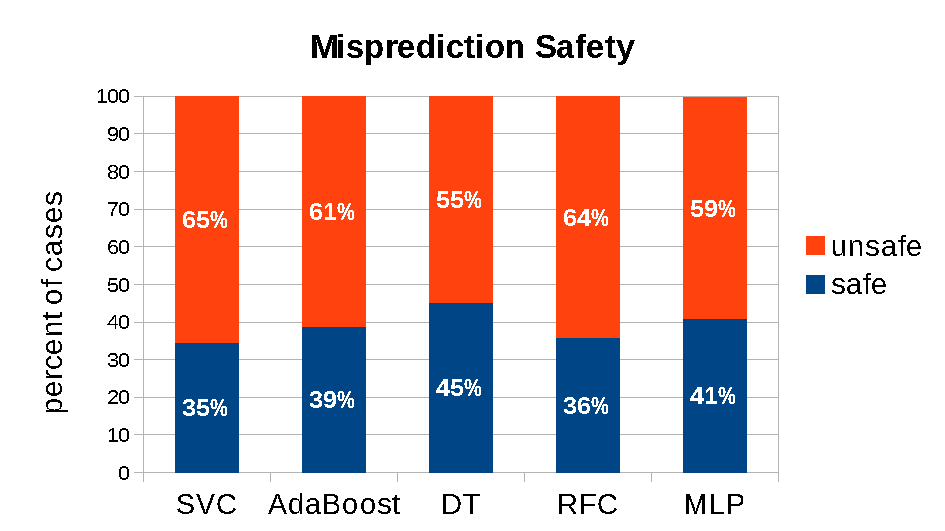
\includegraphics[width=1.0\textwidth]{images/prediction_stats.pdf}
\caption{Breakdown of misclassification errors.}
\label{fig:prediction_stats}
\vspace{-5mm}
\end{figure}
\subsection{Model Performance Within Assistant}
\label{evaluation_loocv}
\quad Our proposed assistant (Section \ref{practical_applications}) is trained and tested using LOOCV rather than K-fold CV. Instead of treating the entire set of loops from all SNU NPB benchmarks as a single data set, in this context we train the model on nine benchmarks and test it on the remaining one. Doing so completely excludes the loops of the target benchmark out of a training set, but allows us to get predictions for all benchmark loops, parallelize them if advised so, and test the effectiveness of our assistant. The drawback of this scheme is that it might potentially reduce the accuracy if the nature of loops in the target benchmark dramatically differs from that of loops seen in the training set. Figure \ref{fig:accuracy_loocv_vs_kfold} compares LOOCV accuracy against that of K-Fold CV for all SNU NPB benchmarks, where K-Fold CV is conducted on a data set consisting of loops from a single benchmark only. The comparison proves that lower LOOCV accuracies are attributed to a reduced training data set and not to our ML model.
\begin{figure}[ht]
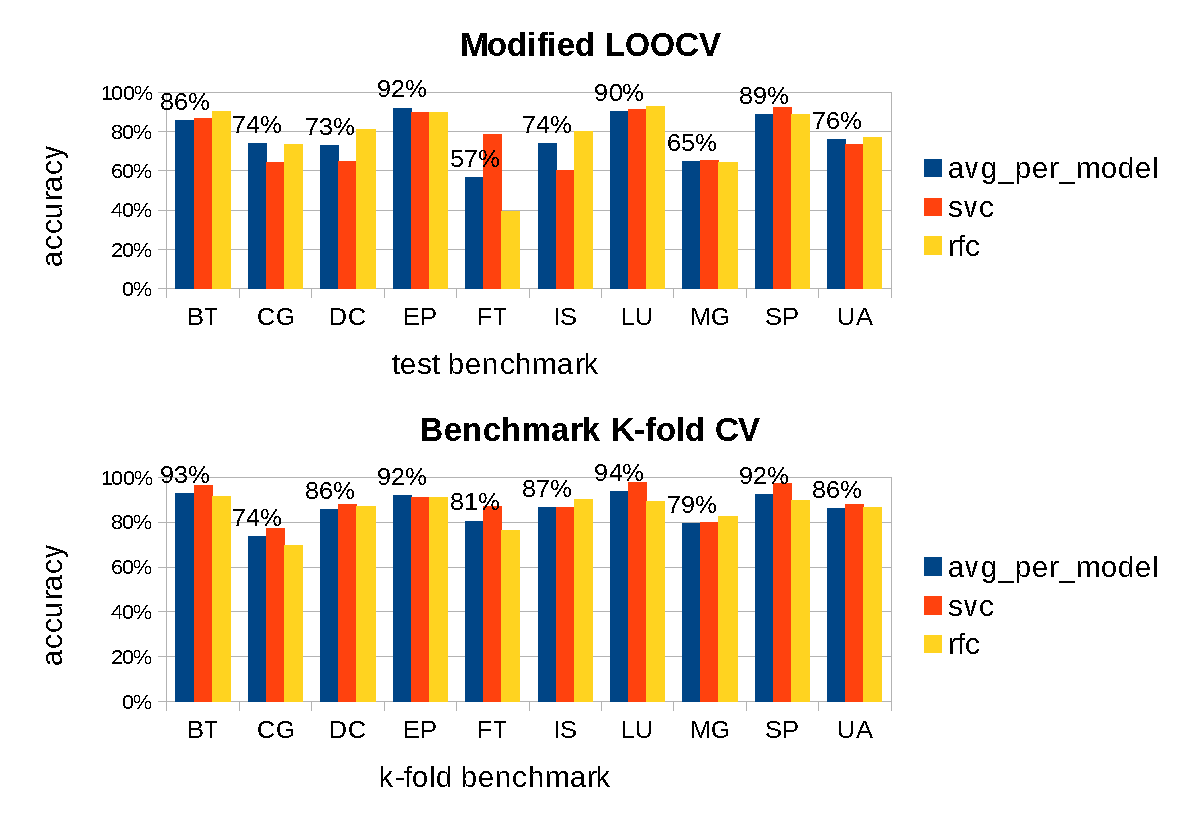
\includegraphics[width=1.0\textwidth]{images/LOOCV_accuracy.pdf}
\caption{Prediction accuracy measured with modified LOOCV and compared against that of K-fold CV for single benchmarks.}
\label{fig:accuracy_loocv_vs_kfold}
\vspace{-5mm}
\end{figure}
\section{Parallelization Assistant}
\label{practical_applications}
\quad Achieving high predictive performance is not enough. We need to find a real practical application of our loop parallelizability predictor. Due to statistical nature inherent to all machine learning techniques it is impossible to eliminate all prediction errors completely. While false negative mispredictions might just miss available parallelization opportunities and lose some performance, false positive mispredictions can break the program and are the most critical in the context of our ML problem.\newlibe\null
\quad Provided above we develop a parallelization assistant, which does not seek to replace programmers, but aims to assist and increase their productivity. The ML-based predictor developed and assessed in the previous two sections is a core component of our novel parallelization assistant. This assistant incorporates prediction results on whether a loop can be parallelized and combines it with profiling information. It then produces a ranking of all loops in an application to guide a programmer towards the most beneficial loop candidates for their \textit{manual} parallelization effort.\newline\null 
\quad \textbf{Loop Ranking.} The loop ranking computed by our parallelization assistant combines a loop's contribution to the overall program execution time with its predicted probability of being parallelizable. In particular, we obtain the ranking by applying a shifted sigmoid function to the predicted parallelizability probability multiplied by the application runtime fraction a loop takes to run as shown in Figure \ref{fig:sigmoid_3d}.
\begin{figure}[ht]
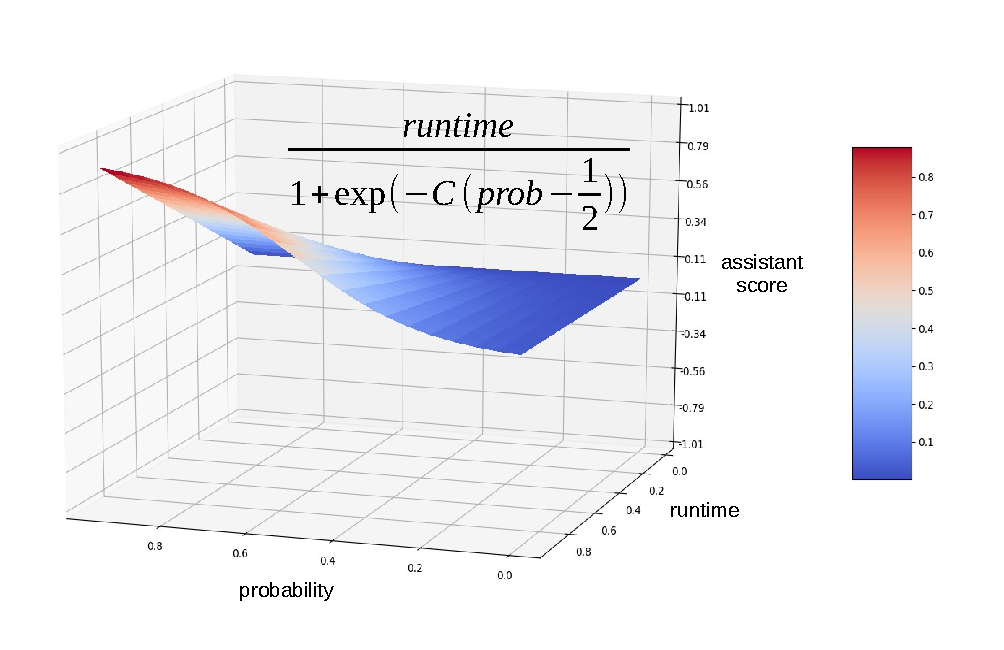
\includegraphics[width=1.0\textwidth]{images/product_func.pdf}
\caption{For each loop the ranking function combines its contribution to the application's execution time and its predicted probability of being parallelizable.}
\label{fig:sigmoid_3d}
\end{figure}
The intuition for using this function to combine the two metrics is that it prioritizes parallelizable long-running loops and scales down the weight of non-parallelizable loops irrespective of their contribution to execution time. The effect of this can be seen in Figure \ref{fig:ft_loop_ranking} for the loops of the FT benchmark.
\begin{figure}[htb!]
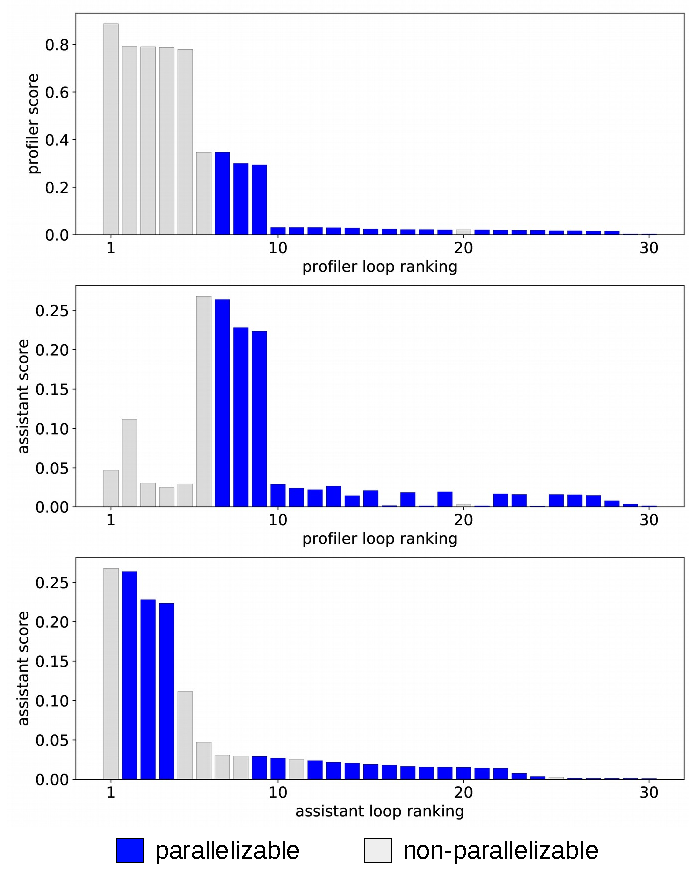
\includegraphics[width=1.0\textwidth]{images/ft_filter.pdf}
\caption{Change of loop rankings with the application of the assistant ranking function for the 46 loops of the FT benchmark. Ranking based on loop execution time alone (top figure) results in some high-ranked, but non-parallelizable loops. Combining profiled execution time and parallelizability in a single score (middle figure) results in a ranking that prioritizes parallelizable loops (bottom figure).}
\label{fig:ft_loop_ranking}
\end{figure}
If programmers attempt to parallelize loops in the order prescribed by their execution time, they will inevitably waste
their efforts trying to parallelize loops which may be long-running, but offer little or no opportunity for extracting parallelism. Instead, by taking into account predicted parallelizability our ranking directly guides the programmer towards loops that significantly contribute to overall execution time \textbf{and} offer a realistic prospect of parallelization.

%Top left and right pictures are identical and rank FT benchmark loops according to their running time score (given by the Intel Compiler). The problem with that order is that it ranks long-running program loops the highest independent of their parallelisability. If a programmer starts to parallelise application following that order, he is going to waste his time and efforts on the loops one cannot parallelise anyway. The left and right plots at the bottom of the figure demonstrate a transformation in the loop ranking our assistant does. Vertical axes of these plots correspond to the values our shifted sigmoid ranking function (see figure \ref{fig:sigmoid_3d}) takes. The bottom left plot shows how the relative height of the bars changes with a switch from a loop runtime to our scoring function. It is clear from the plot, that non-parallelisable loops go down in their importance. The bottom right picture shows that such a change actually moves true parallel loops toward the beginning of the list. The longer loop takes to run, the bigger the move. On the other hand non-parallelisable loops move towards the back of the list (almost independent of their running time). The improved ranking of FT loops allows a programmer to immediately start benchmark parallelisation with the most important loops and don't waste time looking at long-running loops, which cannot be parallelised by their nature anyway.

\subsection{Comparison to Static Analysis} 
\quad We have compared the generated loop parallelizability classifications of our assistant against that of the ICC Compiler, which due to its use of static analysis is conservative and occasionally misses some parallelization opportunities. The ML approach to parallelization with a human programmer responsible for final code transformation allows our parallelization assistant to be more aggressive than the ICC Compiler. In other words, our model can predict more loops as parallelizable. 
\begin{table}
  \tabulinesep=2pt
  \caption{Possible loop classification combinations for the side-by-side setup of our ML predictor and the ICC Compiler.}
  \begin{minipage}{\columnwidth}
  \begin{center}
    \begin{tabu}{M{0.7cm}M{1.4cm}M{3cm}M{5cm}}
      \hline
      \rowfont{\bfseries}
      ICC & Predictor & True Parallel & Classification\\%\hline
      \hline
      0 & 0 & 0 & icc/predictor agreement\\
      0 & 0 & 1 & missed opportunity\\
      0 & 1 & 0 & false positive\\
      0 & 1 & 1 & discovery\\
      1 & 0 & 0 & impossible\\
      1 & 0 & 1 & icc shielding\\
      1 & 1 & 0 & impossible\\
      1 & 1 & 1 & icc/predictor agreement\\\hline  
    \end{tabu}
  \end{center}
  \end{minipage}
  \label{tab:combinations_table}
\end{table}%

We have set up an experiment where we apply our ML predictor side-by-side with the ICC Compiler. Both aim at independently
classifying loops as parallelizable or not. There is a total of six possible classification combinations that our scheme can produce (summarized in Table \ref{tab:combinations_table}). The first and last table rows show the agreement cases, where the ICC Compiler and the ML predictor identically classify truly (non-)parallelizable loops as (non-)parallelizable. The ``missed opportunity'' cases where both ICC Compiler and ML predictor miss parallelizable loops also represent agreement and are not interesting. The most interesting cases are those where the ML predictor and the ICC Compiler disagree. While ICC Compiler is conservative and will never classify a non-parallelizible loop as parallelizible, the statistical ML predictor can make a ``false positive'' error. That works in the opposite direction as well. The ML predictor can discover truly parallelizible loops which escape compiler analysis. These cases are classified as ``discovery'' and have been manually checked in the source code of SNU NPB. The results are summarized in Table \ref{tab:icc_missed_opportunities}, which reports on the reasons behind ICC conservativeness. False negative mispredictions make the ML predictor miss some real parallelization opportunities, but in the fraction of these cases the ICC Compiler can catch them and ``shield'' the ML predictor.
\begin{table}
  \tabulinesep=2pt
  \begin{minipage}{\columnwidth}
  \begin{center}
    \begin{tabu}{M{3cm}M{0.5cm}M{3cm}M{0.5cm}M{3cm}M{0.5cm}}
      \hline
      \rowfont{\bfseries}
      Reason & Num & Reason & Num & Reason & Num\\\hline
      missed reduction & 18 & array privatization & 7 & conservative analysis & 60\\\hline
      unknown iteration number & 7 & static dependencies & 46 & too complex & 22\\\hline
      non-inlined calls & 4 & other & 4 & total & 168\\\hline
    \end{tabu}
  \end{center}
  \end{minipage}
  \caption{Classification of parallelizable loops rejected for parallelization by the ICC Compiler.}
  \label{tab:icc_missed_opportunities}
  \vspace*{-5mm}
\end{table}%

Figure \ref{fig:icc_competition} shows the relative frequency of different loop classification combinations from Table \ref{tab:combinations_table}. We repeatedly ran K-fold CV on the whole set of SNU NPB loops and sorted the outcomes into separate classification buckets from Table \ref{tab:combinations_table}. In 80\% of the cases, our parallelization assistant agrees with the ICC Compiler and classifies truly (non-)parallel loops as (non-)parallel. This is an expected result as we have used ICC (along with OpenMP annotated loops) to train our ML model. However, sometimes our parallelization assistant and ICC reach different conclusions. While there is agreement in the majority of the cases, our tool discovers an additional 10\% of genuine parallelism inaccessible to the ICC Compiler, while allowing 8\% of false positives.

\begin{figure}[t!]
    %\begin{minipage}{\columnwidth}
    \centering
    %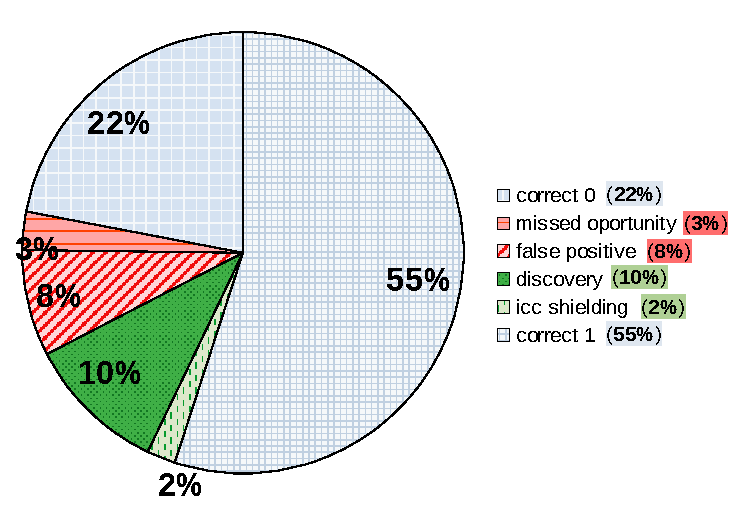
\includegraphics[trim=1mm 1mm 1mm 1mm,clip,width=0.9\columnwidth]{figures/icc_vs_predictor.pdf}
    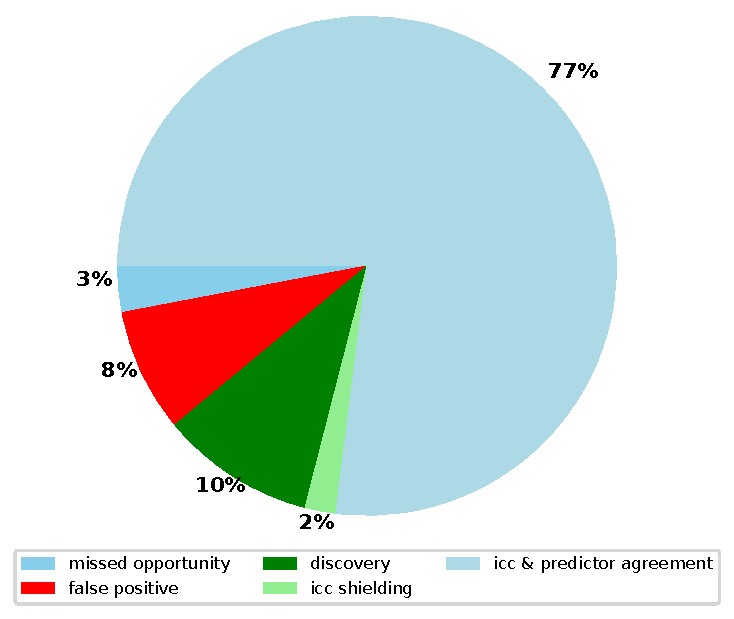
\includegraphics[width=0.9\columnwidth]{images/pie.pdf}
    \caption{
      Distribution of loop classification by the ICC Compiler and our predictor.}
    \label{fig:icc_competition}
%\end{minipage}
\vspace*{-5mm}
\end{figure}

\begin{figure*}[t!]
\centering
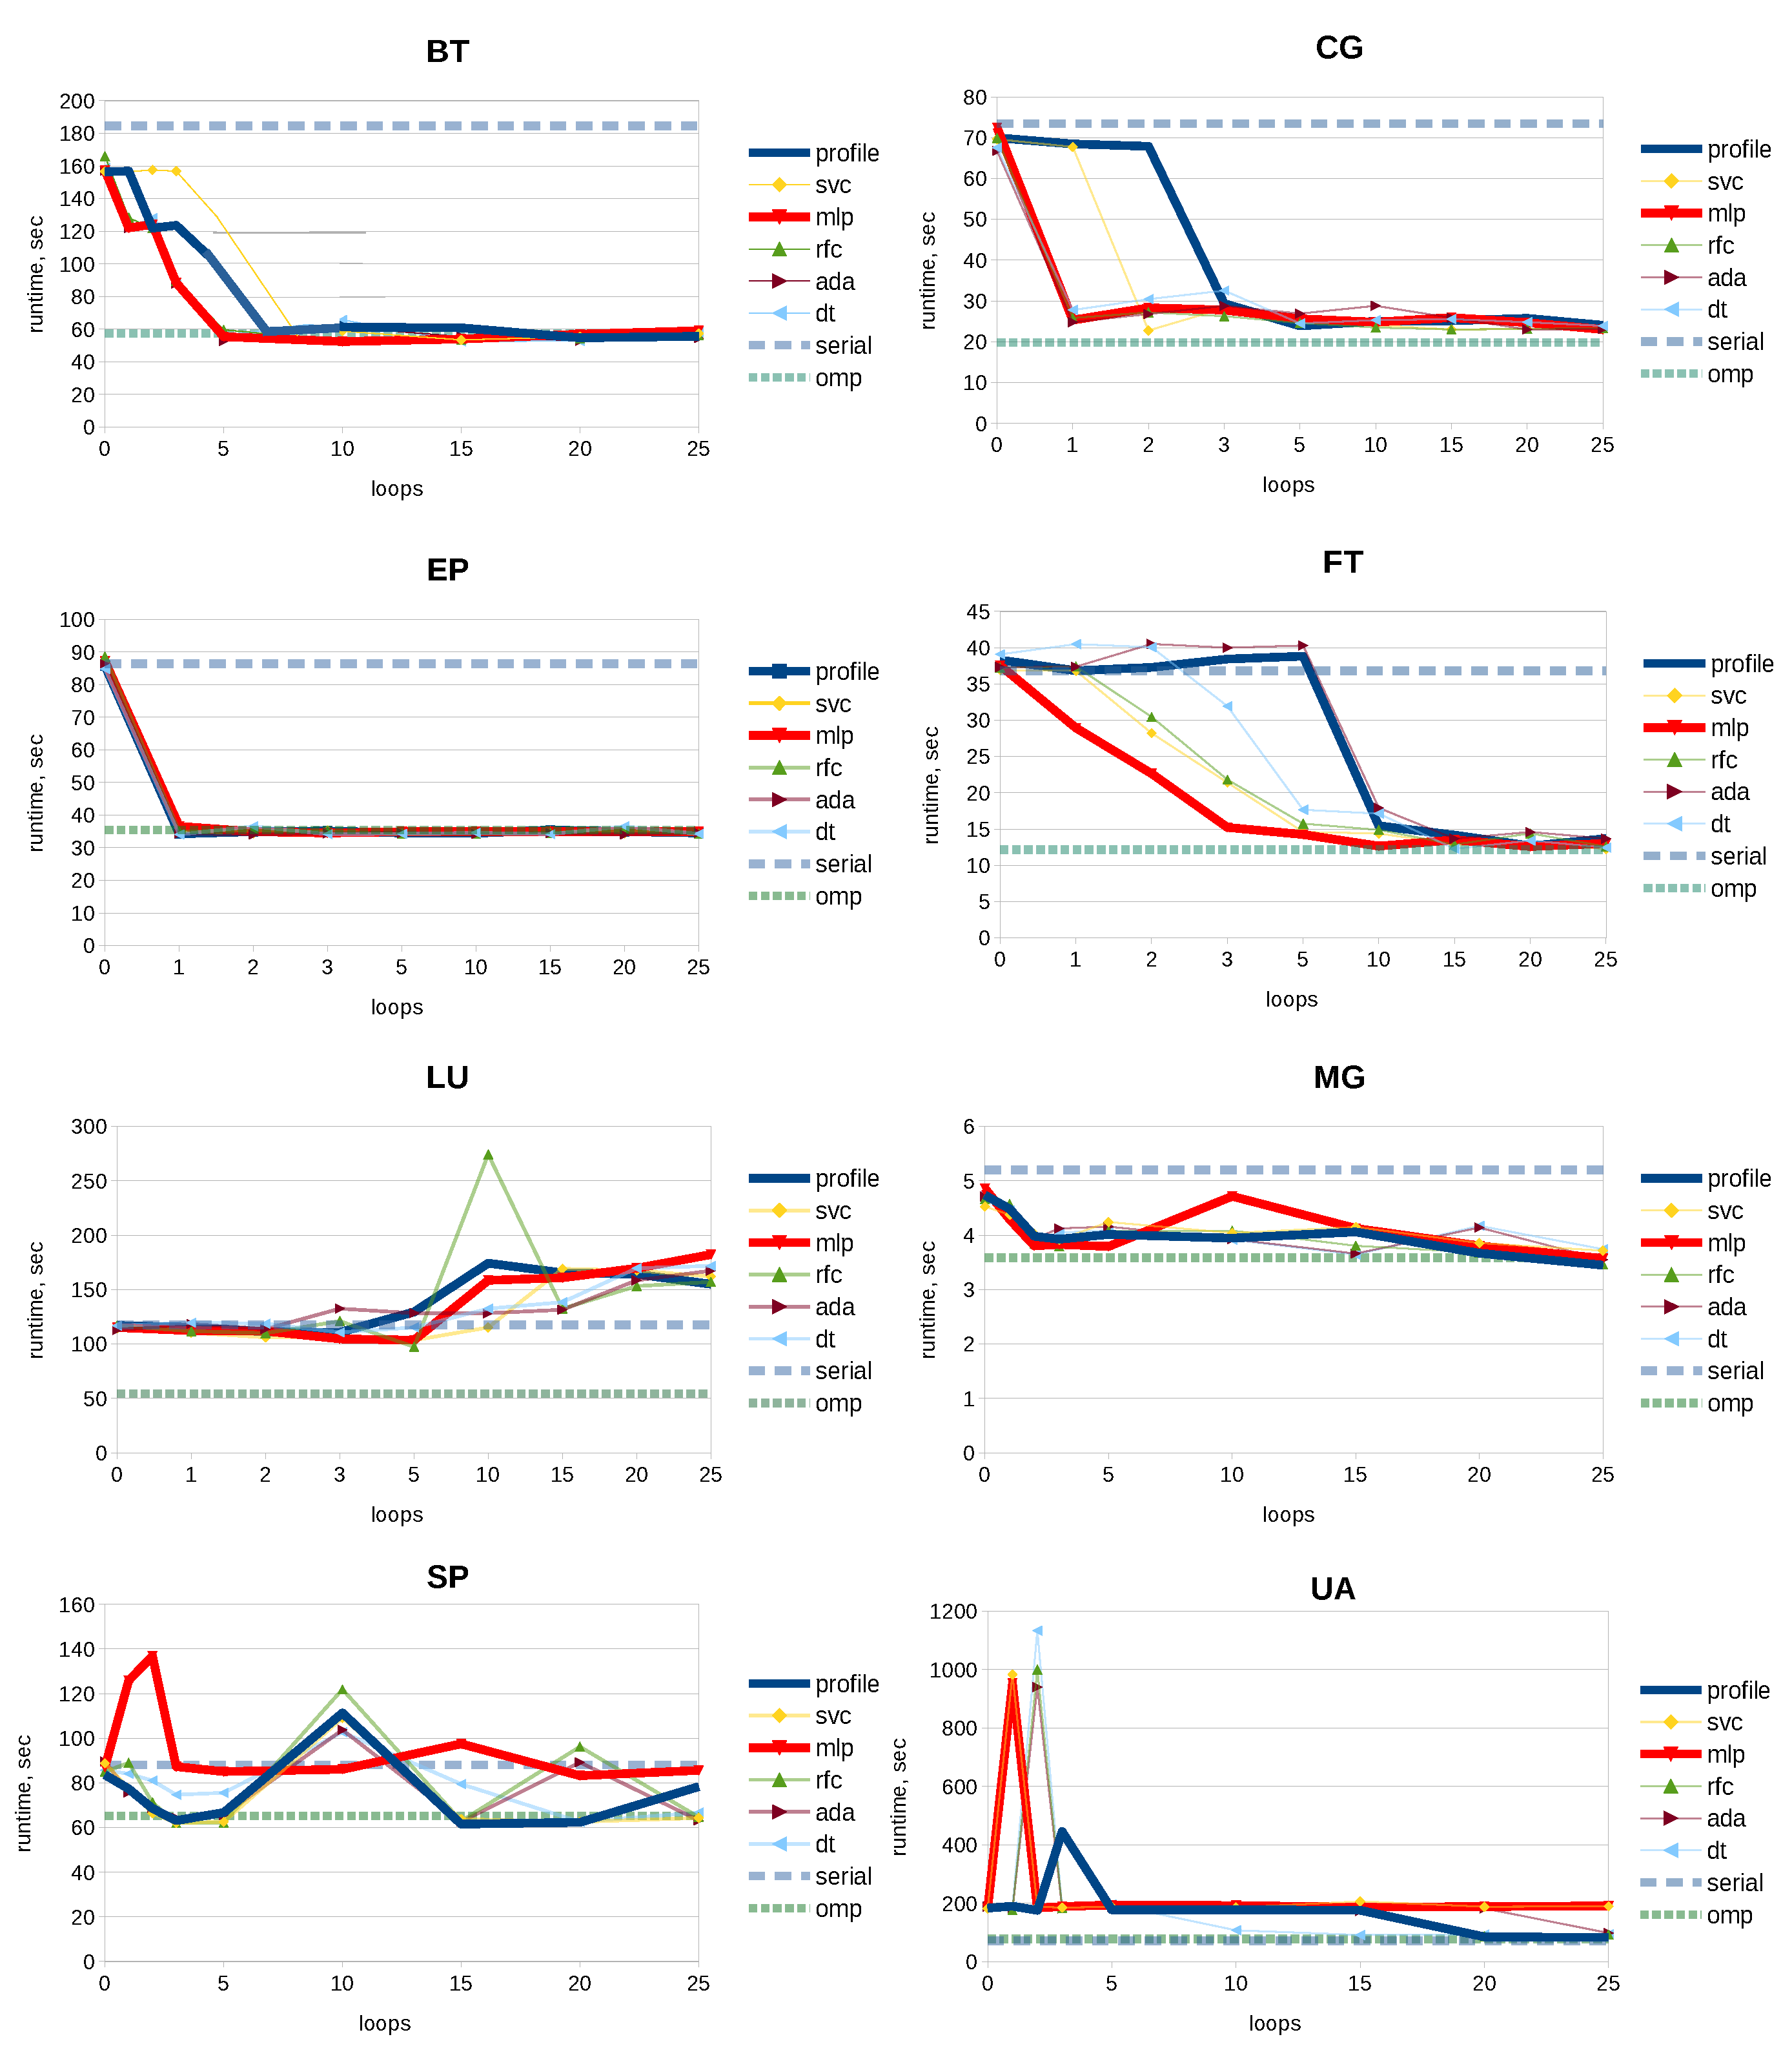
\includegraphics[width=0.95\textwidth]{images/perf_conv_curves_new.pdf}
\caption{From left to right more loops are parallelized for each benchmark. As we parallelize more loops, program execution times improve over the initial sequential performance and reach the performance level of the reference OpenMP implementations. Our ML based parallelization assistant requires the user to parallelize fewer loops than a purely profile-guided approach to reach the maximum parallel speedup.}
\label{fig:performance_convergence_line}
\vspace*{5mm} % Just to fill up the rest of the page
\end{figure*}

\section{Assistant Evaluation}
\label{evaluation}

In this section we evaluate the effectiveness of our parallelization assistant. In particular, we are interested in the potential programmer productivity gains delivered by our tool and savings on human expert time.

Our study assumes that the human expert starts with a sequential version of the SNU NPB benchmarks. The goal
is to parallelize these applications to a performance level matching that of their existing parallel versions.
By using our assistant we expect the human expert to consider fewer loops than by using a profiling-based approach, i.e.\ considering loops in decreasing execution time. We also compare against the state-of-the-art fully automated parallelization approach implemented in the ICC Compiler. The ICC Compiler not only fails to achieve noticeable speedups, but actually slows the performance down on most of the benchmarks. For the BT benchmark the slowdown reaches 3.5 times. In contrast, the OpenMP reference implementation results in a \mbox{(geo-)mean} speedup of 2.19 across the benchmark suite.

Figure~\ref{fig:performance_convergence_line} summarizes our results as
performance convergence curves. For each benchmark the curves plot its execution
time (y-axis) as a function of the number of analyzed and possible parallelized
loops (x-axis). The runtime is bounded within the runtime of the serial
execution (top dashed line) and the time of the reference parallel version (bottom
dashed line). Our goal is to reach the performance of the reference parallel
versions of each program by parallelizing them one loop at a time following the
rankings offered by our assistant and the profiler. The neural network based MLP
model of our assistant provides the fastest overall performance
convergence. While there is some variation depending on the ML model used for
the parallelization prediction, in general ML-assisted parallelization
outperforms or equals the profile-guided schemes across all benchmarks.

Following the rankings of our assistant in parallelizing the BT, CG and FT
benchmarks, we reach their maximum potential performance faster. For BT, maximum
parallel performance can be reached after the user has parallelized the first three 
loops (3061 LOC in Table \ref{tab:parallelization}) suggested by our assistant, while profile-guided parallelization requires 6 loops (6122 LOC) to be parallelized first before reaching the same performance
level. For CG, if we follow the suggestion of our assistant to first parallelize
a small loop (6 LOC), we are able to achieve 70\% of the
maximum potential speedup (see Section~\ref{motivating_example}). On the other
hand, using the profiler ranking requires examining three loops, totalling in
330 LOC, to yield the same performance gains. Moreover, for the SP and UA
benchmarks, some of the assistant rankings require the programmer to examine
more loops than the profiler. However, the loops proposed by the assistant in
the UA benchmark are actually simpler, since they consist of fewer LOC -- 508
LOC for MLP and 579 for DT versus the 882 LOC offered by the profiler. By following our assistant's suggestions, a
programmer would be required to examine 20\% less LOC on average across all models.

%% In general, as it can be seen from Figure \ref{fig:performance_convergence_line} our assistant models perform either better or equal to the profiler. Benchmarks BT, CG and FT gets parallelized to their best OpenMP performance faster by following assistant rankings. In the cases of SP and UA benchmarks some of our assistants require more loops to be examined. However, as Table \ref{tab:parallelization} shows the loops of UA benchmark proposed by our assistants are actually simplier, since they consist of fewer Lines Of Code (LOC) (508 and 579 of MLP and DT against 882 of the profiler). If we calculate the average (across all models) LOC number our assistant would require a programmer to examine and compare that total number against that of a profiler, we see a 20\% reduction.

%% Let's recall a CG benchmark from a motivating example (Section 1). Table \ref{tab:parallelization} shows that the running time of its serial version is 69.38 seconds. SNU NPB provided parallel version takes 19.77 seconds to run. If we follow the ranking of MLP model and parallelize just a small (6 LOC) single loop from the Listing 2, we are going to shorten its execution time to 25.06 seconds (70\% of the maximum speedup). On the contrary, a profiler's ranking would require us to check 3 loops (the total of 330 LOC) to reach the same critical performance level. Full CG benchmark parallelization would bring us 19.77 seconds running time, but we can stop earlier.

In some cases, partial benchmark parallelization might result in a slowdown. In the case of LU, after having parallelized the first 25 loops we do not converge to the best achievable parallel version performance. There are a total of 40 OpenMP pragmas in the benchmark and we need to parallelize all the respective loops to reach the best performance level. In the case of UA, all rankings suggest analyzing a long-running innermost loop first. Its parallelization actually increases running time due to a synchronization barrier being introduced at a wrong program point. It takes 30 loops for the MLP model to achieve the parallel version performance.

\begin{table*}[t]
  \begin{minipage}{\textwidth}
  \begin{center}
\caption{SNU NPB benchmark parallelization reports. The left part of the table shows execution times of serial, OpenMP and partially parallelized (critical) versions. The partially parallelized versions have only several critical (top ranked) loops parallelized. The right hand part of the table shows the number of top-ranked loops one needs to parallelize in order to reach the critical performance. The Profile column gives the reference number a profiler requires. The total lines of code (LOC) in the loops are written down as underscript. In most cases, ML based models converge to the critical performance faster than a profiler based approach (highlighted with green). Red cells show the cases where a profiler outperforms our assistants.}\label{tab:parallelization}
    \begin{tabu}{c|ccc|cc|c|ccccc}
      \hline
      \rowfont{\bfseries}
      \multirow{2}{*}{Bench.} & \multicolumn{3}{c}{Bench.~Runtime, \textit{sec}} \vline & \multicolumn{2}{c}{Speedup, \textit{times}} \vline & \multicolumn{6}{c}{$Loops\ Number_{LOC}$}\\\cline{2-12}
      \rowfont{\bfseries}
      & Serial & OpenMP & Critical & OpenMP & Critical & Profile & SVC & MLP & RFC & AdaBoost & DT\\\hline
      BT & 158.76 & 57.36 & 56.57 & 2.77 & 2.81 & $6_\textit{6122}$ & \cellcolor[HTML]{FA8D8D} $8_\textit{6392}$ & \cellcolor[HTML]{7BB66B} $4_\textit{4088}$ & \cellcolor[HTML]{7BB66B} $5_\textit{5105}$ & \cellcolor[HTML]{7BB66B} $3_\textit{3061}$ & \cellcolor[HTML]{7BB66B} $5_\textit{5105}$\\
      CG & 69.38 & 19.77 & 25.06 & 3.51 & 2.77 & $3_\textit{330}$ & \cellcolor[HTML]{7BB66B} $2_\textit{118}$ & \cellcolor[HTML]{7BB66B} $1_\textit{6}$ & \cellcolor[HTML]{7BB66B} $1_\textit{6}$ & \cellcolor[HTML]{7BB66B} $1_\textit{6}$ & \cellcolor[HTML]{7BB66B} $1_\textit{6}$\\
      DC & 698.82 & 254.29 & 698.82 & 2.75 & 1.00 & $\infty$ & \cellcolor[HTML]{91A1FA} $\infty$ & \cellcolor[HTML]{91A1FA} $\infty$ & \cellcolor[HTML]{91A1FA} $\infty$ & \cellcolor[HTML]{91A1FA} $\infty$ & \cellcolor[HTML]{91A1FA} $\infty$\\
      EP & 86.35 & 35.40 & 35.07 & 2.44 & 2.46 & $1_\textit{45}$ & \cellcolor[HTML]{91A1FA} $1_\textit{45}$ & \cellcolor[HTML]{91A1FA}$1_\textit{45}$ & \cellcolor[HTML]{91A1FA} $1_\textit{45}$ & \cellcolor[HTML]{91A1FA} $1_\textit{45}$ & \cellcolor[HTML]{91A1FA} $1_\textit{45}$\\
      FT & 36.81 & 12.13 & 14.69 & 3.03 & 2.51 & $9_\textit{338}$ & \cellcolor[HTML]{7BB66B} $4_\textit{187}$ & \cellcolor[HTML]{7BB66B} $3_\textit{140}$ & \cellcolor[HTML]{7BB66B} $4_\textit{187}$ & \cellcolor[HTML]{91A1FA} $9_\textit{338}$ & \cellcolor[HTML]{7BB66B} $5_\textit{193}$\\
      IS & 4.75 & 1.35 & 4.63 & 3.53 & 1.03 & $\infty$ & \cellcolor[HTML]{91A1FA} $\infty$ & \cellcolor[HTML]{91A1FA} $\infty$ & \cellcolor[HTML]{91A1FA} $\infty$ & \cellcolor[HTML]{91A1FA} $\infty$ & \cellcolor[HTML]{91A1FA} $\infty$\\
      LU & 115.46 & 55.00 & 140.53 & 2.10 & 0.82 & $\infty$ & \cellcolor[HTML]{91A1FA} $\infty$ & \cellcolor[HTML]{91A1FA} $\infty$ & \cellcolor[HTML]{91A1FA} $\infty$ & \cellcolor[HTML]{91A1FA} $\infty$ & \cellcolor[HTML]{91A1FA} $\infty$\\
      MG & 5.20 & 3.58 & 3.94 & 1.45 & 1.32 & $3_\textit{43}$ & \cellcolor[HTML]{91A1FA} $3_\textit{43}$ & \cellcolor[HTML]{91A1FA} $3_\textit{43}$ & \cellcolor[HTML]{91A1FA} $3_\textit{43}$ & \cellcolor[HTML]{91A1FA} $3_\textit{43}$ & \cellcolor[HTML]{91A1FA} $3_\textit{43}$\\
      SP & 86.65 & 65.19 & 62.90 & 1.33 & 1.38 & $3_\textit{801}$ & \cellcolor[HTML]{91A1FA} $3_\textit{801}$ & \cellcolor[HTML]{FA8D8D} $\infty$ & \cellcolor[HTML]{91A1FA} $3_\textit{801}$ & \cellcolor[HTML]{91A1FA} $3_\textit{801}$ & \cellcolor[HTML]{FA8D8D} $20_\textit{1257}$\\
      UA & 71.82 & 78.56 & 189.66 & 0.91 & 0.38 & $19_\textit{882}$ & \cellcolor[HTML]{FA8D8D} $30_\textit{918}$ & \cellcolor[HTML]{7BB66B} $30_\textit{508}$ & \cellcolor[HTML]{7BB66B} $19_\textit{861}$ & \cellcolor[HTML]{91A1FA} $22_\textit{883}$ & \cellcolor[HTML]{7BB66B} $10_\textit{579}$\\\hline
      \end{tabu}
  \end{center}
\end{minipage}
  %\vspace*{-5mm}
\end{table*}

\begin{comment}
While there is some variation depending on the ML model used for the parallelization prediction, in general ML assisted parallelization outperforms or equals the profile-guided schemes in all benchmarks.
\end{comment}

%% The DC and IS benchmarks are not shown in Figure \ref{fig:performance_convergence_line}. Neither our parallelization assistant nor the profiler reach the performance of the reference OpenMP versions on these benchmarks. Manual inspection reveals that these benchmarks have been parallized using OpenMP parallel sections, but do not contain any OpenMP parallel loops. Both our parallelization assistant and the profiler incorrectly suggest to parallelize some of the benchmark loops, though. The latter leads to the divergence of performance curves and marked with an infinity $\infty$ sign in Table \ref{tab:parallelization}.

Finally, we observe that neither our parallelization assistant nor the profiler
reach the performance of the reference OpenMP versions on the DC and IS
benchmarks. Manual inspection reveals that these benchmarks have been parallized
using OpenMP parallel sections, but do not contain any OpenMP parallel
loops. Both our parallelization assistant and the profiler incorrectly suggest
to parallelize some of the benchmark loops,
though. Table~\ref{tab:parallelization} summarizes the results of applying our
parallelization assistant to the SNU NPB suite.

%are actually demonstrating the deployment of our assistant on SNU NAS Parallel Benchmarks. But before we can assess our assistant we need to conduct a study of performance one could potentially extract from SNU NPB benchmarks. Having measured running times of differently compiled versions, we discovered that ICC compiler not only fails to achieve noticeable speedups, but actually slows the performance down on most of the benchmarks. For BT benchmark the slowdown is striking 3,5 times. Manual expertly done OpenMP parallelisation of SNU NPB developers results into the geomean speedup of 2.19x.\newline\null
%\quad To conduct SNU NPB assistant deployment experiment we had to use a modified LOOCV. For every single SNU NPB benchmark we used the 9 remaining ones to train the predictor and get the ranking of benchmark loops. As section \label{loocv_accuracy} shows such a methodology has a lower predictive performance due to training set incompleteness, which potentially limits the success of our technique. After that we followed the ranking and parallelised the chosen benchmark loop by loop until we managed to achieve the performance level of an expertly parallelised version. We repeated the process for different ML models as well as for a profile based ranking and plotted the performance convergence curves on figure \ref{fig:performance_convergence_line}. Our technique is not applicable to DC and IS benchmarks: these benchmarks get their parallel speedups from OpenMP parallel sections and not from parallel loops. Parallelisation of loops in these benchmarks (be it profile ordered list or the one of our adviser) actually slows them down.  
%\begin{comment}
%\begin{figure*}[th]
%\centering
%\includegraphics[width=\textwidth]{figures/benchmark_runtime.pdf}
%\caption{SNU NPB running times for different compilation options: serial, %automatic parallelisation and vectorization, OpenMP benchmark expert developer %version and all the possible combinations of those.}
%\label{fig:snu_npb_performance}
%\end{figure*}
%\end{comment}
%\begin{comment}
%\quad The common general thing about all SNU NAS benchmarks we observed is %that the main portion of benchmark speedup comes from a coarse-grain manual %parallelisation done by its developers. The main loops preceded by OpenMP %pragmas are quite big and complex. Usually they contain calls to different %%functions, which do not always get inlined, as well as a lot of %multidimensional arrays with complex index computations. Many array references %happen indirectly and thus require runtime behaviour knowledge for their %analysis. Parallelisation of such loops requires a thorough comprehension of %the source code by a programmer, and is beyond the capabilities of the %state-of-the-art automatic tools.\newline
%\quad Intel compiler vectorises and parallelises quite a significant number of %SNU NAS benchmark loops, but these loops are not the main ones. When we %measure the performance of parallel and vector codes generated by Intel %compiler, we observe running times being slightly better than in serial %versions for vector codes and significant slowdowns for automatic ICC %parallelisation.       
%\quad The major weakness of Intel compiler, as well as our trained loop %parallelisability classifier is that they mostly discover relatively %fine-grain parallelism and miss opportunities seized by manual coarse-grain %parallelisation. SNU NAS benchmarks contain a lot of big loops with deep %nesting and uninlined function calls inside. SNU NAS developers have deep %benchmark behaviour understanding and know exactly where even such loops can %be parallelised, but that knowledge is far beyond the sight of automatic %tools. 
%\quad Parallelism present in EP and DC benchmarks is undetectable neither by %Intel compiler nor by our oracle. DC benchmark contains only 1 parallel %section encapsulating many function calls and complex control flow. Such %parallelism cannot be detected in principle. Performance of EP benchmark %depends heavily on the single loop with a reduction. SNU NPB developers have %successfully manually parallelised this loop, but neither ICC nor trained %oracle could find parallelism in it. Oracle predicted thsi loop to be 40\% %parallelisible. The loop is complex and contains 2 inner loops, where %reduction variables are buried as well as timer and random generator function %calls.\newline
%\quad Our scheme does not utilise all the coarse-grain parallelism of FT %benchmark as well. Developers parallelise outermost loops of loop nests, %whereas our classifier finds parallelism only in a modestly-sized inner loops, %which do not contain function calls (thus operating at a finer level). Such %finer parallelisation is not always beneficial and introduces overheads from %implicit OpenMP barriers.
%\quad Our scheme advised us to parallelise almost all BT benchmark loops, %which contain OpenMP pragma in the original hand-parallelised benchmark %version. There are a couple of missed OpenMP pragmas. Moreover, our scheme %advises us to parallelise inner loops with a finer grains of parallelism, but %doing so results in a slowdown, rather than speedup. So we take predictor's %feedback and apply it on the top of our common sense that only outer loops %should be parallelised to avoid synchronisation overheads and stalls.    
%\end{comment}

\section{Related Work}
\label{related_work}

%We focus our discussion of related work on contributions, which are related to the ML aspects of the approach presented in this paper.

\textit{Profitability Analysis.}
The SUIF \cite{Wilson:1994:SIR:193209.193217} parallelizing compiler uses a simple heuristic based on the product of statements per loop iteration and number of loop iterations to decide whether a parallelizable loop should be scheduled to be executed in parallel. In contrast, Tournavitis \emph{et al.}~\cite{Tournavitis:2009:THA:1542476.1542496} use a machine learning based heuristic, which incorporates \textit{dynamic} program features collected in a separate profiling stage, to decide if and how a potentially parallel loop should be scheduled across multiple processors.

\textit{ML in Compiler Optimization.}
Machine learning has been used to solve a wide range of problems, from the early successful work of selecting compiler flags for sequential programs, to recent works on scheduling and optimizing parallel programs on heterogeneous multi-cores. Some works for machine learning in compilers look at how, or if, a compiler optimization should be applied to a sequential program. Some of the previous studies build supervised classifiers to predict the optimal loop unroll factor \cite{4907653,1402082} or to determine whether a function should be inlined \cite{Zhao2003ToIO,1559966}. These works target a fixed set of compiler options, by representing the optimization problem as a multi-class classification problem where each compiler option is a class. Evolutionary algorithms like generic search are often used to explore a large design space. Prior works~\cite{Almagor:2004:FEC:997163.997196,Cooper:2005:AAC:1065910.1065921,Ashouri:2017:MMC:3132652.3124452} have used evolutionary algorithms to solve the phase ordering problem (i.e.\ in which order a set of compiler transformations should be applied).

\textit{Machine Learning and Parallelization.}
Most relevant to the work presented in this paper is the approach of Fried \emph{et al.}~\cite{fried_ea:2013:icmla}. Similar to our approach, Fried \emph{et al.} train a supervised learning algorithm on code hand-annotated with OpenMP parallelization directives in order to approximate the parallelization that might be produced by a human expert. However, we do not rely solely on OpenMP annotations, but we complement our training set with substantially richer data obtained from an aggressively configured parallelizing compiler. While Fried \emph{et al.}~focus on the comparative performance of different ML algorithms, we contribute a practical parallelization assistant capable of ranking loop candidates in their order of merit. Through this we directly enhance programmer productivity in an ML-assisted environment. Similarly to our approach, Hayashi \emph{et al.}~\cite{Hayashi:2015:MPH:2807426.2807429} extracts various program features during compilation for use in a supervised learning prediction model. However, its aim is the optimal runtime selection of CPU vs. GPU execution and it is limited to programs written in Java using the parallel stream APIs that was introduced in version 8.

\section{Summary \& Conclusions}

In this paper we contribute a methodology and tool for parallelization assistance. We acknowledge that parallelization is a complex process where the human expert still has a major role to play. We aim to assist the human experts by guiding them directly towards the most interesting loops, thus delivering savings for this costly human resource. We have developed a novel machine learning based approach to predicting whether or not a loop is parallelizable. We combine this prediction with traditional profiling information and develop a ranking function that prioritizes low-risk, high-gain loop candidates, which are presented to the user.

We have evaluated our parallelization assistant against the sequential C implementations of the SNU NPB suite. We show that our assistant recognizes parallelizable loops more aggressively than conservative parallelizing compilers. We also show that our parallelization assistant can increase programmer productivity. Our experiments confirm, that equipped with our assistant, a programmer is required to examine and parallelize substantially fewer loops to achieve performance levels comparable to those of the reference OpenMP implementations of the benchmarks.

Our work has demonstrated that there is scope for machine learning based tool support in parallelization despite its inherent lack of safety. By assisting human programmers rather than replacing them, machine learning techniques have the potential to deliver productivity gains beyond what is possible by relying on traditional parallelization approaches alone.

\section*{Acknowledgements}

This work was supported by grant EP/L01503X/1 for the University of Edinburgh School of Informatics Centre for Doctoral Training in Pervasive Parallelism. We would like to thank Artemiy Margaritov and Kuba Kaszyk for their valuable feedback on earlier drafts of this paper. Finally, we would like to thank the anonymous reviewers for their comments and suggestions.

%The ultimate goal of this work has always been to provide a programmer with a feedback on the parallelisability of software in general and loops in particular. The work has evolved from parallelisability correlations of single metrics (features) to a machine learning based tool for filtering runtime program profile and providing the resulting loop ranking for a programmer.\newline\null
%\quad The ultimate performance of the tool depends on many factors. First 

%\subsection{Future Work}

%Having received some motivating results, there are still certain areas of improvement. The tool consists of a number of co-designed parts. Their tuning for maximum overall performance can be done infinitely. The ultimate performance of the tool is affected by a number of factors. The main factor is the nature of the programs (benchmarks) being used for ML training and testing stages. SNU NAS benchmarks are quite diverse in terms of the loops they contain. Loops have different sizes, nesting structures, parallelism patterns.

%\quad We believe, that our idea can be worked on and improved even further. There are several possible potential steps.

%\quad Our scheme consists of a number of components and steps. First we select training and testing programs, then we engineer the set of representative ML features. After 

%\quad First, SNU NPB benchmarks have certain features and properties that reveal themselves in our work. 
%\quad In our work we use SNU NAS Parallel Benchmarks for assessment of our machine learning based technique. Majority of SNU NPB benchmarks concentrate their running time in a relatively small set of critical loops. That fact presents a problem for a full scale assessment of our technique.      



%Our tool consists of a lot of components to be tuned. The tuning work can be done infinetely in the attempt to get the best possible performance on a wider range of programs and benchmarks.    

% \subsection{Future Work}









\chapter{Computational Frameworks}
\label{frameworks}
\section{Overview}
\label{frameworks_overview}
\quad The problem of \textit{parallel software development} is multifaceted. To arrive at the final solution, a programmer has to work on multiple conceptual levels starting from problem decomposition and algorithm choice down to software architecture design, data structure choice, and finer-grained low-level loop transformations. If our loop parallelization assistant (see Chapter \ref{assistant}) aims at reducing the programmer's effort in the task of parallelizing a sequential program, the notion of computational frameworks and the library implementing it could be used in the process of developing a parallel application from the scratch. The solution we propose rids the programmer of the tasks of software architecture design, as well as algorithm and data structure choice by supplying a ready solution for parallelization of certain types of applications. The central motivating ground for the concept of computational frameworks is laid by the \textit{Data-Centric Parallelization (DCP)} problem, limitations of the related work, and the properties of the real world legacy codes.
\begin{center}
\textbf{\large \textit{Motivating ground for Computational Frameworks}}
\end{center}
\begin{description}[style=unboxed,leftmargin=0cm]
\itemsep0em
\item[\textit{The grand problem of Data-Centric Parallelization (DCP)}] Among all lower level implementation questions, the problem of successful data structure choice stands particularly prominent and important. Listings \ref{lst:frameworks_array} and \ref{lst:frameworks_list} illustrate how easily parallelization can be hampered. Both implementations solve an embarrassingly parallel problem of incrementing every sequence element by one. In the linear array based implementation compiler knows all element addresses statically and can generate parallel code. In the linked list based implementation compiler does not know element addresses in advance, since the latter will be resolved only dynamically and can generate only sequential code. Moreover, the data structure type is unknown to compiler. By parallelizable and non-parallelizable loops here we mean the loops that can and cannot be parallelized by the state-of-the-art compiler statically.\newline\null
\begin{minipage}[t]{0.5\linewidth}
\begin{lstlisting}[caption={\raggedright Parallelizable loop operating on what is clear to compiler a \textbf{linear array}.},label={lst:frameworks_array},language=C]
int a[1024];
for (int i=0; i<1024; i++) {
  a[i]=a[i]+1;
}
\end{lstlisting}
\end{minipage}
%
\begin{minipage}[t]{0.5\linewidth}
\begin{lstlisting}[caption={\raggedright Non-parallelizable loop operating on what programmer knows is a \textbf{linked-list}.},label={lst:frameworks_list},language=C]
struct Node* nptr;
for (p=nptr; p!=NULL; p=p->next) {
  p->value+=1;
}
\end{lstlisting}
\end{minipage}

If a programmer had a tool, that could automatically recognize the type and properties of data structures and automatically substitute them with a simpler, parallelizable and more suitable alternatives, that would make the parallelization process a lot easier. Unfortunately, as our state of the art overview discovered, the solution to the problem is not available yet. There are a lot of various techniques and methodologies with their specific limitations and problems.
\item[\textit{Data structure and algorithm inseparability}] An illustrative example in Listings \ref{lst:frameworks_array} and \ref{lst:frameworks_list} is obviously far below the complexity level of the real world code. The work with data structure can be spread all around the code base: allocation and initialization happen in one translation unit, update operations on the data structure are scattered between various functions in multiple other translation units. The exact way an operation works determines the properties (cyclicity, reachability, etc.) of a data structure and ultimately its type. It is crucial to understand how an algorithm actually calls data structure update operations. \textit{This all points to the inseparability of algorithms and data structures: understanding the type of the data structure might require understanding of the algorithm and vise versa; and the data structure substitution might lead to algorithm transformation.} Indeed, as our feasibility studies with the SPEC CPU2006 benchmark suite have shown (Section \ref{background_benchmarks_spec}) let alone automatic techniques, it might take some weeks for even an experienced human software engineer to understand what kind of data structures a benchmark uses and how to optimize it.
\item[\textit{Limitations of "The state of the art" work}] The discovery of higher level entities in programs is definitely not a novel idea. There are various \textit{static} and \textit{dynamic} techniques in the literature. \textit{Shape analysis} is one of the most well-known static techniques, which aims at understanding of various heap-allocated data structures and their properties (node reachability, cyclicity, disjointedness, etc.) at compile time \cite{Ghiya:1996:TDC:237721.237724}\cite{Sagiv:1999:PSA:292540.292552}\cite{Wilhelm:2000:SA:647476.760384}). \textit{Shape analysis techniques give a very rough and conservative approximation (a \textit{tree} instead of a \textit{linked list}), work with high error rates (\textit{DAG} instead of \textit{graph with cycles}) and are provably undecidable \cite{Muchnick:1998:ACD:286076}}. One of the more recent static techniques is based on pattern matching on the code intermediate representation (IR) level and aims at recognition of various computational idioms (such as reductions, stencils, sparse and dense linear algebra computations, etc.)\cite{Ginsbach:2017:DEG:3049832.3049862}\cite{Ginsbach:2018:CDS:3178372.3179515}\cite{Ginsbach:2018:AML:3296957.3173182}. Computational idioms are specified in a constraint-based domain specific programming language CAnDL. \textit{The technique allows for a rapid prototyping of new compiler optimizations based on pattern recognition and its substitution with an optimized versions of matched idioms, but it is limited for a relatively simple computational idioms and entities.} All static methods are limited in their program view to a single compilation unit. The challenge of data structure recognition requires a much broader view. Dynamic techniques come the closest to the solution of the DCP problem. There are numerous works available \cite{Haller:2016:SDS:2938006.2938029}\cite{Rupprecht:2017:DID:3155562.3155607}. These techniques are based on program instrumentation and construction of various dynamic memory allocation graphs. The idea is that these graphs along with their update operations can reflect the actual shape of the data structure. Probably, the most promising and the best performing of all is the work of a Data-structure Detection Tool (DDT) \cite{1669122}. The DDT tool can successfully recognise data structures in most of the standard libraries, such as STL, Apache (STDCXX), Borland (STLport), GLib, Trimaran achieving almost perfect recognition accuracy. Moreover, the technique has been able to recognise linked lists in Em3d and Bh Olden benchmarks. But, it is still far from solving the problem for an arbitrary real world code.
\item[\textit{The ongoing trend to higher abstraction levels}] For decades there has been an ongoing trend in the process of software engineering to move up in the levels of abstraction from bare hardware to higher level concepts closer to human reasoning and understanding. We have moved from assembly languages to languages like Fortran and C, followed by the development of object-oriented languages and a supplement of imperative programming languages with functional programming concepts. All these steps increase programmers productivity, improve program structuredness and modularity and move the process of software design closer to a human level. The trend of moving to higher abstraction levels is not only true for software engineering in general, but for parallel software engineering in particular. For example, standards like POSIX, OpenMP and MPI aim at abstracting a programmer from various hardware and operating system details and work on the level of platform agnostic parallel programming models. Parallel algorithmic skeletons \cite{mccool-patterns} (see Section \ref{background_skeletons}) move software parallelization process even higher and allow a programmer to specify a computation on the algorithmic level with various concepts like \textit{map}, \textit{stencil}, \textit{divide and conquer}, etc.
\end{description}
\begin{center}
\textbf{\large \textit{A higher level solution}}
\end{center}
\quad The task of separating data structures from algorithms for an arbitrary real world code is extremely challenging. Moreover, for some applications and benchmarks it does not seem meaningful either. For example, the suite of Olden benchmarks is much simpler, than SPEC CPU2006, but also exhibits the same inseparability problem. For many of Olden benchmarks the data structures and algorithms are blended, but the union they form can be framed into an elegant higher level entity, that can later be used to parallelize the benchmarks in a nice and structured way.\newline\null
\quad In this thesis we propose a novel notion of \textit{computational frameworks}, which exploit this possibility and help a programmer with a coarse-grained parallelization tasks, such as software design, algorithm and data structure choice on applications, where computations can be expressed with our computational frameworks. We describe the concept and the major frameworks in Section \ref{frameworks_main}. We provide a prototype C++ template library implementing the notion \cite{frameworks-repo} (see Section \ref{frameworks_library_design}). We prototyped the library on the suite of Olden benchmarks, which inspired and shaped the concept. The parallel library version consistently outperforms the sequential version hitting 5-6x speedups on the major benchmarks (see Section \ref{frameworks_performance}).
\subsection{Contributions of our Computational Frameworks}
\begin{itemize}[style=unboxed,leftmargin=0cm]
\itemsep0em
\renewcommand\labelitemi{$\vartriangleright$}
\renewcommand\labelitemii{$\bullet$}
\item We propose a novel notion of \textit{computational frameworks}, which are higher level entities that embody both data structures and algorithms; and
\item report on a prototype C++ template library \cite{frameworks-repo} implementing the notion in a modern, convenient, parallel and an easy to use way;
\item We express the computations of some Olden benchmarks in terms of our computational frameworks and rewrite their original sequential legacy C versions with the help of our library in a modern, better structured, portable and crucially parallel way (see Section \ref{frameworks_main});
\item We demonstrate the potential of the notion and the performance of the prototype library on the suite of Olden benchmarks (see Section \ref{frameworks_performance}), achieving consistent parallel speedups of 5-6x on the major benchmarks;
\item Finally, we propose an idea of alternative software parallelization approach based on our computational frameworks as a future work.
\end{itemize}
\section{Usage example}
\label{frameworks_usage_example}
\quad To get an initial feeling for what it is like to use our computational frameworks from a user perspective, let's consider a motivating example. A full discussion of the concept follows in Section \ref{frameworks_main}. Suppose we want to calculate a well-known functional programming concept of the \textit{right fold}, which also updates its elements with corresponding folded values, thus leaving some \textit{side effects}.\newline\null
\quad We can code that simple computation using the C++ Standard Template Library (STL). Listing \ref{lst:left_fold_list} shows the code implementing the task with an STL $list<> $ class template. First, we construct a list with 5 elements and initialize them to the value of 1. Then we loop through the list updating its elements and return the final right folded value. The task is small and the code is concise, but it is still possible to see its drawbacks. The code does not clearly separate concerns: list traversal, result computation and list transformation all happen in the same place and are mixed up together. For a better structuredness and comprehensibility it would make sense to put these different pieces of functionality into separate places. Alternatively, we could use STL's $std::accumulate()$ function template. The latter provides a programmer with a more concise and abstract interface, but does not allow any side effects. We would still need to write a separate chunk of code aimed at implementing an update of the list elements.\newline\null 
\quad Listing \ref{lst:left_fold_framework} shows an alternative implementation of the right fold using our \textbf{Fold} computational framework. The main computation here is expressed with a single line of code and a reader familiar with the concept of fold will comprehend the purpose of the code instantly. The fold defines the backbone of the computation, which is hidden from a user, while the definition of the custom part is left for a user to complete and is passed into a higher order functional style interface $Fold<Elem>::compute()$ as a function object $ComputeFunc$, which has been derived from a Fold-specific base class $Fold<Elem>::ComputeFunction<int>$. The latter is a template with the main computational result specified as a parameter. The base class frames the interface. Operator $Fold<Elem>::ComputeFunction<int>::operator()(Elem\&,int)$ takes an element of the Fold as an argument and combines it with the value folded so far in a user defined way. The user is supposed to pass the result further and has a freedom to update the element, thus leaving some side effects. The code in Listing \ref{lst:left_fold_framework} has a clear structure, but might feel a bit heavy for such a simple computation, but when a computational task is significant the advantages of the shown code design will become clear.

%\begin{minipage}[t]{\linewidth}
\begin{lstlisting}[caption={Right fold computation using standard STL list class template},label={lst:left_fold_list},language=C++]
#include <list>
using namespace std;

int main() {
    list<int> lst(5, 1);
    // lst = [ 1 <- 1 <- 1 <- 1 <- 1 ]
    
    int result = 0;
    for (auto it = lst.rbegin(); it != lst.rend(); it++) {
        *it += result;
        result = *it;
    }
    // lst = [ 5 <- 4 <- 3 <- 2 <- 1 ]
    // result = 5
    
    return 0;
}
\end{lstlisting}
%\end{minipage}

%\begin{minipage}[t]{\linewidth}
\begin{lstlisting}[caption={Right fold computation using our Fold computational framework},label={lst:left_fold_framework},language=C++]
#include "Fold.h"
using namespace abstract;

class Elem : public Fold<Elem>::Element {
    public:
        void grow() override { value = 1; }
        int value;
};

class ComputeFunc : public Fold<Elem>::ComputeFunction<int> {
    int operator()(Elem& elem, int fold) override {
        elem.value += fold;
        return elem.value;
    }
};

int main() {
    int fold_depth = 5;
    Fold<Elem> fold(fold_depth);
    // fold = [ 1 <- 1 <- 1 <- 1 <- 1 ]
    
    int result;
    ComputeFunc comp_func;
    result = fold.template compute<int>(comp_func);
    // fold = [ 5 <- 4 <- 3 <- 2 <- 1 ]
    // result = 5
    
    return 0;
}
\end{lstlisting}
%\end{minipage}

\section{Computational Frameworks}
\label{frameworks_main}
\quad In this section we describe the general concept of \textbf{computational framework} along with all frameworks we propose and implement in the prototype library. As our frameworks have been inspired by computations found in the Olden benchmark suite, it would be helpful to review the Section \ref{background_benchmarks_olden} describing the key benchmarks.
\subsection{The concept}
\label{frameworks_concept}
\quad As we have already mentioned the concept of \textit{computational framework} has been inspired by the current problems in the software parallelization field along with computational patterns we have observed in the suite of Olden benchmarks. Very often programs are written with sub optimal from the point of software parallelization data structures. It might be hard to substitute them with parallelizable alternatives as the former might be closely entangled with algorithms the program is based on. Hence:
\begin{itemize}[style=unboxed,leftmargin=0cm]
\itemsep0em
\renewcommand\labelitemi{$\vartriangleright$}
\renewcommand\labelitemii{$\bullet$}
\item Computational frameworks grow on the problem of data structure and algorithm inseparability;
\end{itemize}
\quad We might keep the two together, but still tackle the problem at a higher level. We call the higher level entity we operate with a computational framework. Computational emphasizes the algorithmic component, while framework hints towards the underlying data structure. 
\begin{itemize}[style=unboxed,leftmargin=0cm]
\itemsep0em
\renewcommand\labelitemi{$\vartriangleright$}
\renewcommand\labelitemii{$\bullet$}
\item Computational frameworks combine algorithms and data structures to form a higher level entity;
\end{itemize}
\quad Moreover, there are some specific problems, that could be tackled more effectively with specialized constructs. Imagine some task of scientific simulation. The scientific computation might be abundant with various higher level algorithmic constructs like maps, reductions, folds, stencils, etc. These concepts are characteristic of functional programming. The latter often forbids any mutable states. At the same time simulations often keep a significant state being updated and accumulated with every step. The presence of state is characteristic to an imperative programming. Here one can see a contradiction and hence the gap to fill: \begin{itemize}[style=unboxed,leftmargin=0cm]
\itemsep0em
\renewcommand\labelitemi{$\vartriangleright$}
\renewcommand\labelitemii{$\bullet$}
\item Computational frameworks fill the gap between imperative and functional programming paradigms;
\end{itemize}
\quad With all the things said above it is human programmers, who are going to use the concept in the end. Hence, it must be human friendly and convenient. At the same time the code must be modern and effective. We designed an object-oriented library with a functional style interface consisting of higher order functions. While the algorithmic component of the given framework is immutable there is a custom user defined functionality to apply to the framework. That functionality comes as a function object through the framework's interface in accordance with a command and template method (see Section \ref{background_design}) software design patterns. 
\begin{itemize}[style=unboxed,leftmargin=0cm]
\itemsep0em
\renewcommand\labelitemi{$\vartriangleright$}
\renewcommand\labelitemii{$\bullet$}
\item Computational frameworks provide a modern and convenient interface with elements of both functional, as well as object-oriented programming; and
\item Computational frameworks embody the best ideas of various software design patterns. 
\end{itemize}
\quad When the software architecture has been designed, the exact efficient algorithm has been chosen along with all the most optimal and suitable data structures supporting its operation, a programmer can move onto the task of software parallelization. Here:  
\begin{itemize}[style=unboxed,leftmargin=0cm]
\itemsep0em
\renewcommand\labelitemi{$\vartriangleright$}
\renewcommand\labelitemii{$\bullet$}
\item Computational frameworks implement an effective and portable parallelization under the hood.
\end{itemize}
\quad To conclude:
\begin{itemize}[style=unboxed,leftmargin=0cm]
\itemsep0em
\renewcommand\labelitemi{$\vartriangleright$}
\renewcommand\labelitemii{$\bullet$}
\item Computational frameworks improve program \textbf{structuredness}, \textbf{modularity}, \textbf{separation of concerns} and hide possible \textbf{program parallelization} behind the \textbf{modern and convenient} user interface. 
\end{itemize}
\subsection{Fractal}
\label{frameworks_fractal}
\quad The \textbf{Fractal} computational framework is the key framework in our work. It has been inspired by the theoretical work on tree reductions \cite{tree-reductions-paper} and 3 Olden benchmarks (\textit{health}, \textit{treeadd} and \textit{perimeter}) with a very similar computational pattern. Although, the work on tree reductions has laid the theoretical foundation, but it did not provide a practical implementation. While there are numerous computations, processes and examples, which can be framed into the fractal, for the simplest and the most illustrative example let's consider an n-ary tree data structure being processed as follows.\newline\null
\quad \textbf{Fractal's growth.} First, we grow the tree from the root down to its leaves. A node takes a seed to grow, grows and spawns the next set of seeds for all its children nodes. The latter continue the process of growth. In the most general case the growth can happen asymmetrically, i.e it can stop on some paths down the tree, when some user specified condition is met for some nodes. In other words, the tree becomes incomplete with some leaves growing deeper than others and some nodes not having some children. We saw that pattern in the \textit{perimeter} benchmark (see Section \ref{background_benchmarks_olden}), when squares fell completely outside or inside the ring, they stopped to split further. Benchmarks \textit{health} and \textit{treeadd} grow complete trees and do not specify any stop conditions. While the algorithmic pattern of growth is fixed, the node's growth itself along with the node's data are custom and user defined parts. The same is true of the type of seeds and seed spawning procedures. Moreover, the growth of the tree along its various branches happens independently and can be parallelized.\newline\null
\quad \textbf{Fractal's processing.} When the tree is grown, we can start to process it. On that stage we go in the opposite direction from the bottom up by starting to process the leaves of the tree first. For every node we do some custom computation along with updating its custom data and pass the computation's result up to its parent. Before we process any node we need to process all its children first. The processing of different children happens independently and can safely be parallelized. When the tree has been processed we obtain the final result from its root along with all the side effects left in the nodes of the tree. The user defines these side effects per node in the custom processing function along with defining the exact computation from children up to the parent. We can repeat the process numerous times. This is the way some simulations work. The side effects are going to accumulate and make the nodes heavier.
\begin{figure}[!htb]
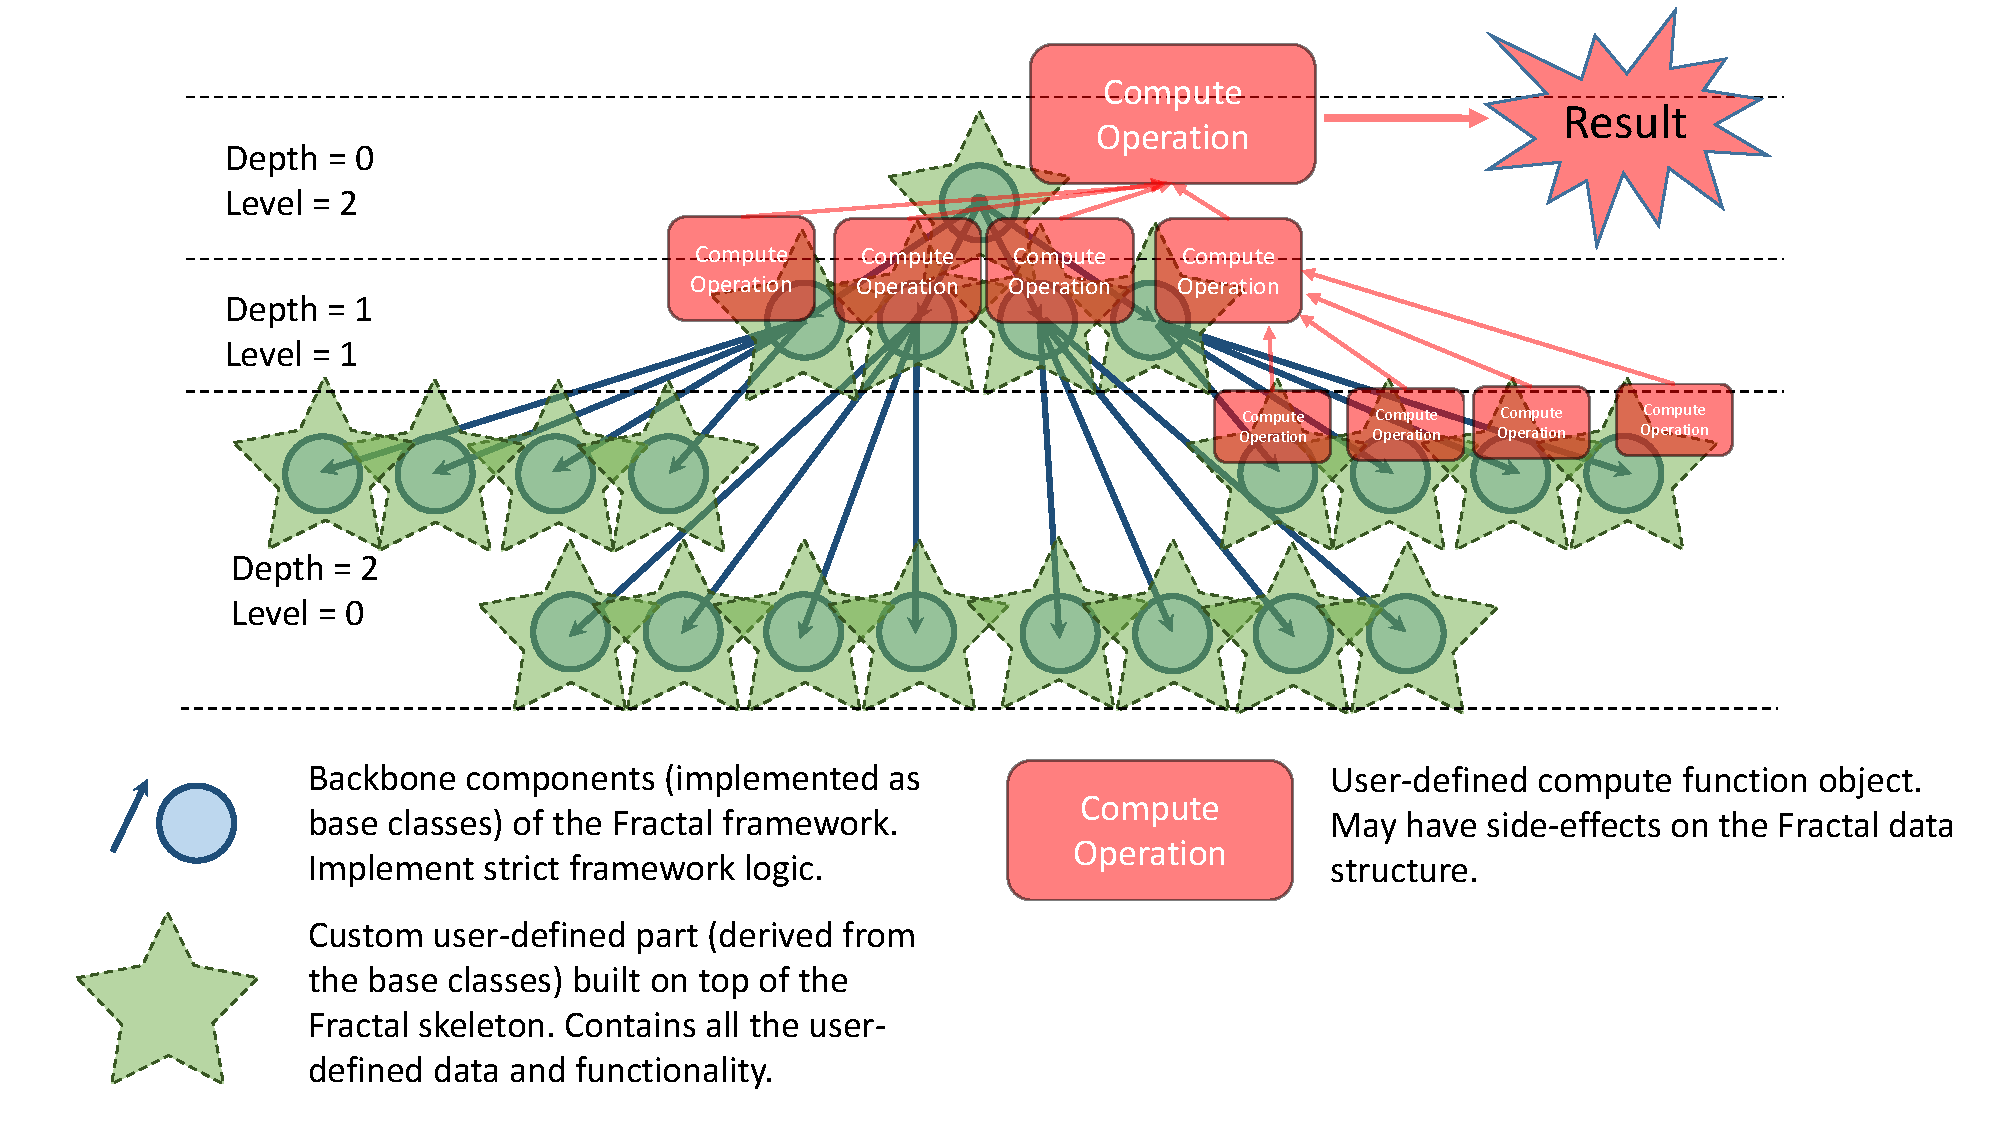
\includegraphics[width=1.0\textwidth]{images/Fractal.pdf}
\caption{Our object-oriented design of the Fractal computational framework.}
\label{fig:fractal_scheme}
\end{figure}
Figure \ref{fig:fractal_scheme} illustrates the pattern described above, as well as proposes an object-oriented design of the fractal concept. The backbone components (circles and arrows) of the tree are immutable and keep the main computational and growth patterns. These components can be implemented as base classes. Along with the backbone logic implementation these base classes provide a customizable interface to be overriden by derived classes (stars). Derived classes specify custom data contained in the tree nodes along with the exact growth and processing procedures, which can touch and alter the data. Given the fixed custom data in the tree nodes, computations operating on the data may still vary. We customize computations as function objects (red rectangles) being passed into higher order functional interfaces of the fractal. In other words, our fractal provides functional style interfaces above its object-oriented structure with the main backbone logic hidden under the hood. The backbone logic can be implemented sequentially or be parallelized in a multiple ways. In all its generality the fractal is a pattern, which can be characterized with self-similarity, repeatedness, structuredness, inherent parallelizability and the exact numeric values such as its depth and arity.
\subsection{Fold}
\label{frameworks_fold}
\quad The \textbf{Fold} computational framework has been inspired by the computation done in the \textit{power} benchmark (see Section \ref{background_benchmarks_olden}). The fold is not a new concept and has found a wide application in many functional languages. The C++ language provides \textit{std::accumulate()} function template as a component of its Standard Template Library (STL), which performs a functional fold over a given data structure, but contrary to our computational framework it does not allow any side-effects and modifications to the elements of the data structure must be coded separately. Our C++ \textit{Fold} class template provides an alternative interface to a user with an extensible customization space and clear separation of concerns.\newline\null
\begin{figure}[ht]
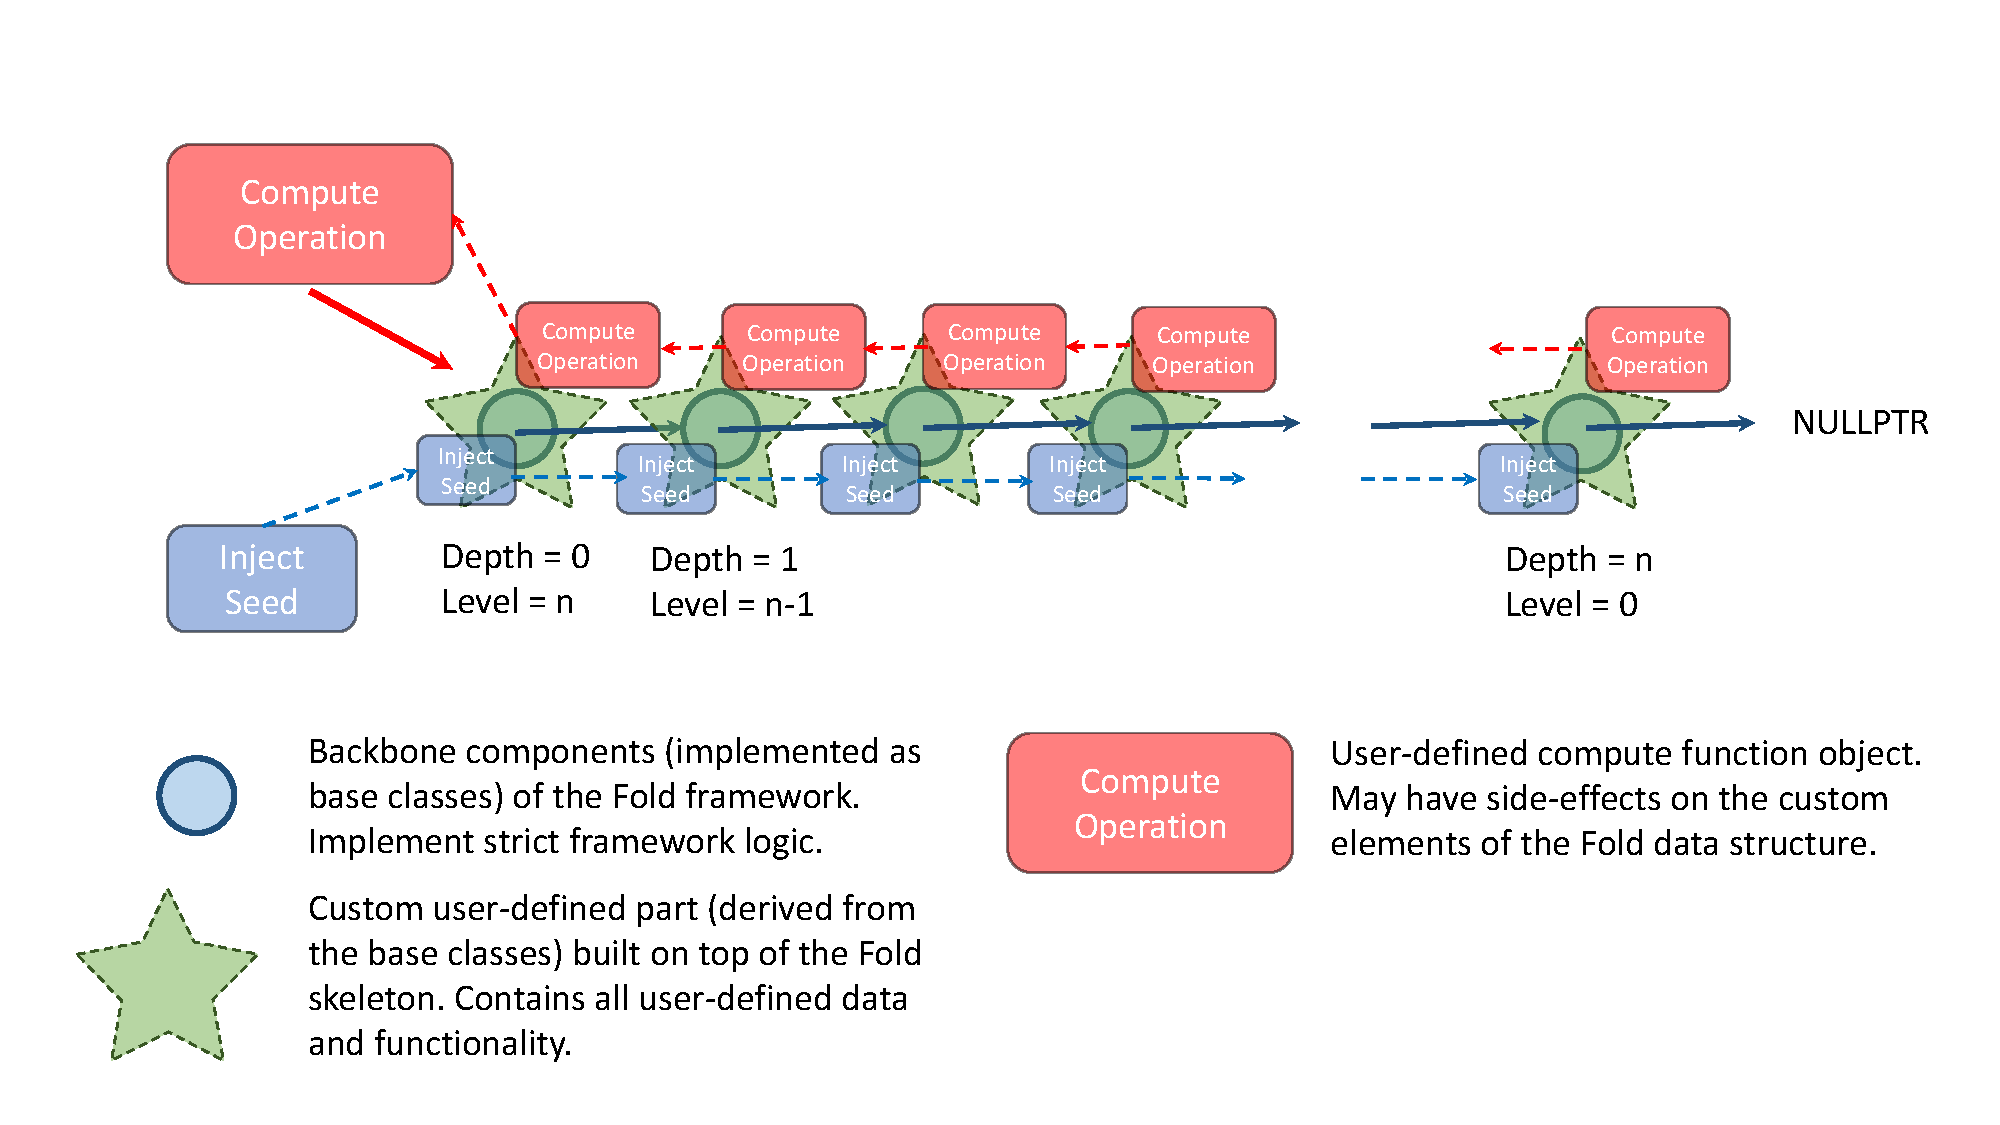
\includegraphics[width=1.0\textwidth]{images/Fold.pdf}
\caption{An object-oriented design of the Fold computational framework.}
\label{fig:fold}
\end{figure}\newline\null
\quad Figure \ref{fig:fold} illustrates the framework. One can think of a Fold as a set of elements arranged into a linked-list. We grow the list to the specified depth given a seed value. Then we may inject some data into the head of the list and propagate the data along with its custom changes to the last element at the tail of the list. All propagation modifications are user-defined. The injection of the data might happen as needed (before every fold iteration for example). Once every element of the list is ready with its injected data planted, the computation starts at the tail element and passes computed values back to previous elements of the chain. The computation may leave some side effects on the elements of the fold, which can accumulate with fold repetitions. The pattern is not parallelizable, but defines a strict order and helps to structure the code to separate various concerns. The object-oriented design of the fold framework is coherent to that of the fractal. Base classes form the skeleton logic and define the interface. All customization happens through overriding inherited base class interface methods withing definitions of derived classes. Custom compute operation is a function object going into functional interfaces of higher order \textit{Fold} class methods.
\subsection{Reduce}
\label{frameworks_reduce}
\quad Strictly speaking, \textbf{Reduce} is not a computational framework, but an algorithmic skeleton (see Section \ref{background_frameworks_vs_skeletons}). Although it is implemented with exactly the same design and interface, what illustrates compatibility between the two closely related concepts. The difference between our framework and \textit{std::reduce()} from C++ Standard Template Library (STL) is the possibility of having side effects and an alternative user customization interface. All general remarks made regarding \textbf{Fold} and \textbf{Fractal} frameworks also apply to the \textbf{Reduce} framework, although the specific details might differ. For example, the reduce framework takes a function object with two overloaded and virtual \textit{operator()} methods. One specifies how to reduce the value from a single element (possibly changing the element in the process) and the other defines the way of combining all the reduced values into the final return value. Our framework implements sequential as well as parallel \textbf{Reduce} versions.
\begin{figure}[ht]
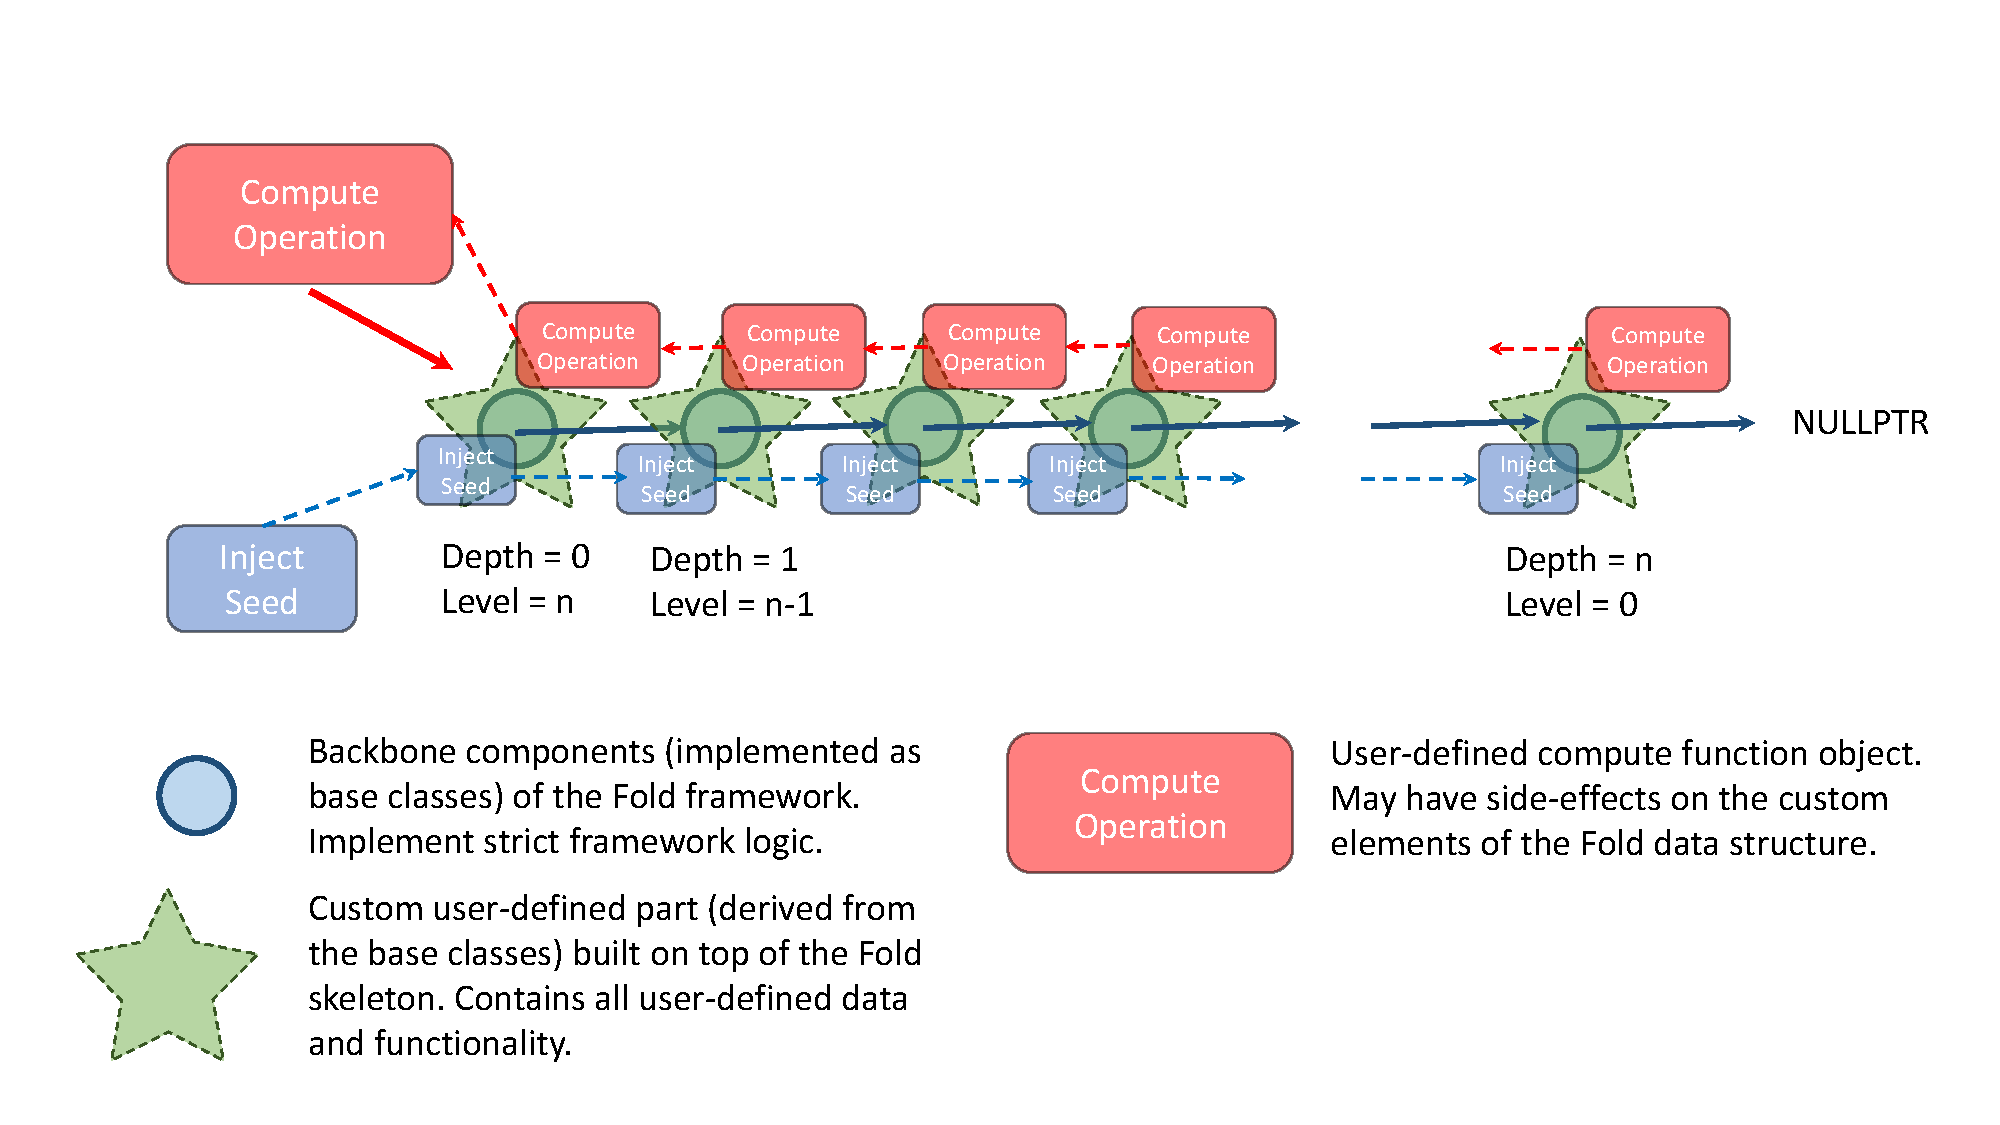
\includegraphics[width=1.0\textwidth]{images/Fold.pdf}
\caption{An object-oriented design of the Reduce algorithmic skeleton. The design is identical to that of computational frameworks. The two concepts are inter-operable.}
\label{fig:reduce}
\end{figure}
\subsection{Frameworks library design and implementation}
\label{frameworks_library_design}
\quad Despite a number of framework specific differences, all our frameworks stick to the same user interface and design. The design and implementation of computational frameworks library have been done along the curved and iterative path running into numerous dead ends and doing redesign efforts over and over before we managed to get the final library version \cite{frameworks-repo}. The major questions raised during the design process of the library were the trade-off between employing static vs. dynamic polymorphism, interoperability of different frameworks (how do we handle the reduction of folds of folds of reductions like in the case of the \textit{power} benchmark, for instance?), as well as the overall library coherence questions (how to design a common interface for patterns as different as fold and fractal?). But the final design goals have always been clear and follow below.
\begin{description}[style=unboxed,leftmargin=0cm]
\itemsep0em
\item[Modern C++] The implementation of the library is based on the Standard Template Library (STL) data structures, uses move semantics and unique pointers to achieve efficiency and smart memory management. For parallelization library uses OpenMP standard, thus making source code portable. The library is composed of a set of header files with class templates, which are supposed to be included into the user application.
\item[Convenience] We designed the library in an object-oriented fashion with a functional look of its user interfaces and the portability in mind.
\item[Coherence] Despite variations in the prescribed behaviour, all computational frameworks should stick to the same user interface as well as internal design. The coherence would improve inter-operability of different frameworks (say composing a reduction of folds), improve library usability, as well as ease its maintenance and extension. Among less intuitive things, a more general design that handles folds, reductions, fractals, etc. along with all the applications using them altogether will be of the higher quality overall.
\item[Sound design] We strove to use the best software design practices. The user side of the library has been inspired by the LLVM Pass Framework \cite{llvm-compiler-infrastructure} and alike it the library uses the \textit{Curiously Recurring Template Pattern (CRTP)} to decrease the number of template parameters and avoid some of the dynamic polymorphism overheads. The concept of computational frameworks fits exactly into the well-known \textit{algorithm template} pattern and the functional user side is implemented with function objects and higher order template methods following the \textit{command} pattern.
\end{description}
\quad We used 4 Olden benchmarks as an inspiration and guide. Benchmarks \textit{health}, \textit{perimeter} and \textit{treeadd} defined our \textbf{Fractal} computational framework. The \textit{power} benchmark shaped \textbf{Fold} and \textbf{Reduce} frameworks. Moreover, striving for coherence and common interface, the designs of different frameworks had a profound effect on each other.\newline\null
\quad Listing \ref{lst:framework_template_skeleton} shows the essential parts of the final framework design. Initially, custom framework element growth methods such as $Element::grow()$ and $Element::growth\_stop\_condition()$ were specified as separate $Framework<>$ template parameters, but were moved to become virtual functions of the base $Element$ class as a trade-off between static vs. dynamic polymorphism. The template method $Framework<>::compute<ComputeType>()$ is a higher order functional interface, which takes a function object of framework specific type $Framework<>::ComputeFunction<>$ and applies it to the framework along with computing the main result of the $ComputeType$ type. Listing \ref{lst:framework_template_skeleton} shows the one for \textbf{Reduction} class. A user is supposed to override two overloaded operators(), which specify a reduction from a single element complemented with the final combining operation. $Framework<>::grow()$ method defines the backbone data structure and representation of the framework and makes calls to custom user defined functions controlling the growth process.

%\begin{minipage}[t]{\linewidth}
\begin{lstlisting}[caption={Computational framework class template skeleton},label={lst:framework_template_skeleton},language=C++]
template <typename ElemType, typename SeedType>
class Framework {
    public:
        class Element {
            // user-exposed customization iface
            virtual void grow(SeedType) = 0;
            virtual bool growth_stop_condition() { return false; }
        };
        template <typename ComputeType>
        class ComputeFunction {
            public:
            // framework specific application function API
            virtual ComputeType operator()(ElemType& elem) = 0;
            virtual ComputeType operator()(const std::vector<ComputeType>&) = 0;
        };
        void grow(size_t size, SeedType seed) {
            // organise framework elements 
            // into a data structure
            ... = new ElemType(); 
        }
        template<typename ComputeType>
        ComputeType compute(ComputeFunction<ComputeType>& apply_func);
    
    private:
        // framework data structure organisation
        // (list, tree, array, etc.)
};

\end{lstlisting}
%\end{minipage}
\section{Library Deployment}
\label{frameworks_performance}
\subsection{Source Lines Of Code (SLOC) metric  comparison}
\label{frameworks_loc}
\quad Although the Source Lines Of Code (SLOC) metric does not always correctly reflect program properties (such as comprehensibility, maintainability, etc.), it is still interesting to compare the original legacy C implementation of Olden benchmarks against the implementation based on our computational frameworks in terms of this metric.\newline\null
\quad Here we need to make some comments. First, the comparison is not completely fair, since the original pointer-based implementation of Olden benchmarks is sequential (only \textit{power} benchmark contains parallelizing OpenMP pragmas). Whereas our implementation can be made sequential or parallel with just one line of code (like \textit{tree.set\_impl\_type(Fractal\_t::ImplType::parallel)}) and everything else happens "under the hood". It is also important to note, that we are comparing legacy C vs. C++ implementations. Programs written in C++ tend to be slightly more verbose in terms of SLOC with their class definitions, constructors, destructors, extra keywords, etc. Second, as with any third-party library, before we can use it, we need to perform a setup, which often contains a lot of "boilerplate" code. In the case of computational frameworks, the setup implies the derivation of custom classes from the base classes of our library, instantiating templates, and some other extra syntactical constructions. The business logic of the application can be split into two phases: computational framework \textit{build} and \textit{compute}.\newline\null
\begin{table*}[!ht]{\linewidth}
  \tabulinesep=2pt
  \begin{minipage}{\linewidth}
  \begin{center}
    \begin{tabu}{M{1.4cm}M{1.2cm}M{1.2cm}M{1.2cm}M{1.2cm}M{1.2cm}M{1.2cm}M{1.2cm}M{1.2cm}}
      \hline
      \rowfont{\bfseries}
      \multirow{2}{*}{stage} & \multicolumn{2}{M{2cm}}{power} & \multicolumn{2}{M{2cm}}{health} & \multicolumn{2}{M{2cm}}{perimeter} & \multicolumn{2}{M{2cm}}{treeadd}\\
      & original & abstract & original & abstract & original & abstract & original & abstract\\\hline
      setup & 80 & 170 & 55 & 65 & 15 & 35 & 10 & 30\\
      build & 60 & 50 & 50 & 30 & 50 & 60 & 15 & 1\\
      compute & 380 & 460 & 250 & 230 & 190 & 200 & 60 & 40\\\hline
      \end{tabu}
  \end{center}
  \caption{Implementation SLOC size comparison: original legacy C version (\textit{original}) vs. C++ computational frameworks based one (\textit{abstract}). }
  \label{tab:frameworks_sloc}
  \end{minipage}
\end{table*}%
\quad Table \ref{tab:frameworks_sloc} presents the results. For all 4 benchmarks, the setup size is larger in terms of SLOC for the implementation based on our computational frameworks, but after the setup is done we can see some improvement on the \textit{health} and \textit{treeadd} benchmarks. Parallel C++ version of the benchmarks takes less SLOC than a legacy sequential one. The \textit{power} benchmark demonstrates the opposite tendency. The computation of the benchmark is composed of the reduction of folds of folds of reductions. Moreover, every fold contains two components: left inject and right fold. These joint points require some additional setting, initialization, and passing of parameters. While this improves the separation of concerns and program structuredness, it bloats the code as a side effect. The \textit{perimeter} benchmark does not show significant differences.
\subsection{Performance study of the library}
\label{frameworks_runtime}
\quad To assess the potential and utility of the concept of computational frameworks, we implemented a prototype library and conducted its thorough performance examination on the subset of Olden benchmarks. We used 4 benchmarks we are interested in. Benchmarks \textit{health}, \textit{treeadd} and \textit{perimeter} fit into our \textbf{Fractal} framework and stress it from different angles. We used the \textit{power} benchmark to test the practical operation of our \textbf{Fold} and \textbf{Reduce} frameworks. We expressed computations in these benchmarks through applicable computational frameworks and have rewritten the original sequential legacy C implementations of the benchmarks with our prototype library in a rejuvenated, structured, well-designed and crucially parallel way. On the opposite side, these benchmarks inspired the concept of computational frameworks and shaped the design of the library. \textit{All our benchmarks have been compiled with GCC 10.1 and -O3 optimization sets. Benchmark running times have been measured with the help of UNIX \textbf{time()} on a powerful compute cluster running Ubuntu 20.04 (focal) and having 64 AMD EPYC 7302 3303 MHz 16-core processors with a total of 0.5 Tb of RAM}.\newline\null
\quad Performance plots below (Figures \ref{fig:performance_health}, \ref{fig:performance_power_reduction_width}, \ref{fig:performance_treeadd}, \ref{fig:performance_perimeter}) show the strengths of the library, as well as its equally important weaknesses. The latter characterize applicability and limitations of the library, rather than the problems of the idea. Although \textit{perimeter} benchmark still demonstrates the potential it also highlights the prototype research nature of the library and shows where it needs an optimization effort. The latter presents a matter of software engineering and not that of a research.\newline\null
\quad The implementation can be easily configured to be sequential or parallel, thus making it easy to conduct measurement experiments. Moreover, the Fractal framework has 2 implementations under the hood. In the most general case the Fractal is based on N-ary unbalanced tree. In this case we allocate it dynamically and every node has an array of pointers to its children. But in the case of a perfect (all leaves are at the same depth and every non-leaf node has all children present) tree, we can allocate all nodes linearly in an array-based heap manner. In the latter case parallelization happens per level, spawning the number of threads equal to the number of nodes at the given depth (provided that enough CPU cores are available). In the general case though we do not know where the growth of the fractal is going to stop and cannot index nodes on the array. Parallelization in the case of unbalanced fractal happens per child: spawning the number of threads equal to the number of children (again, provided that enough CPU cores are available). Figure \ref{fig:balanced_vs_unbalanced} illustrates two implementation strategies and performance plots below compare them. Listing \ref{lst:fractal_parallelization} illustrates "under-the-hood" parallelization of our fractal computational framework in the most general case of unbalanced tree. Parallelization happens only at the topmost level to limit the number of threads spawned.
\begin{lstlisting}[caption={The "under-the-hood" parallelization of unbalanced Fractal computational framework},label={lst:fractal_parallelization},language=C++]
template <typename ElemType, typename SeedType, int Arity>
template <typename ComputeType>
ComputeType Fractal<ElemType,SeedType,Arity>::Element::compute(ComputeFunction<ComputeType>& compute_func) {
    
    std::vector<ComputeType> ret_vals;
    
    if (!children.empty() && 
        (this->info.level-1 > 0) )
    { 
        if (info.depth < 2) {
            ComputeType tmp[Arity];
            int threads_count = Arity;
            #pragma omp parallel num_threads(threads_count) shared(tmp)
            {
                #pragma omp for schedule(static)
                for (int i = 0; i < Arity; i++) {
                    tmp[i] = children[i]->template compute<ComputeType>(compute_func);
                }
            }

            for (int i = 0; i < Arity; i++) {
                ret_vals.push_back(tmp[i]);
            }
        } else {
            for (int i = 0; i < Arity; i++) {
                ret_vals.push_back(children[i]->template compute<ComputeType>(compute_func));
            }
        }
    }
   
    return compute_func(*(static_cast<ElemType*>(this)), ret_vals);
}
\end{lstlisting}
\begin{figure}[!htb]
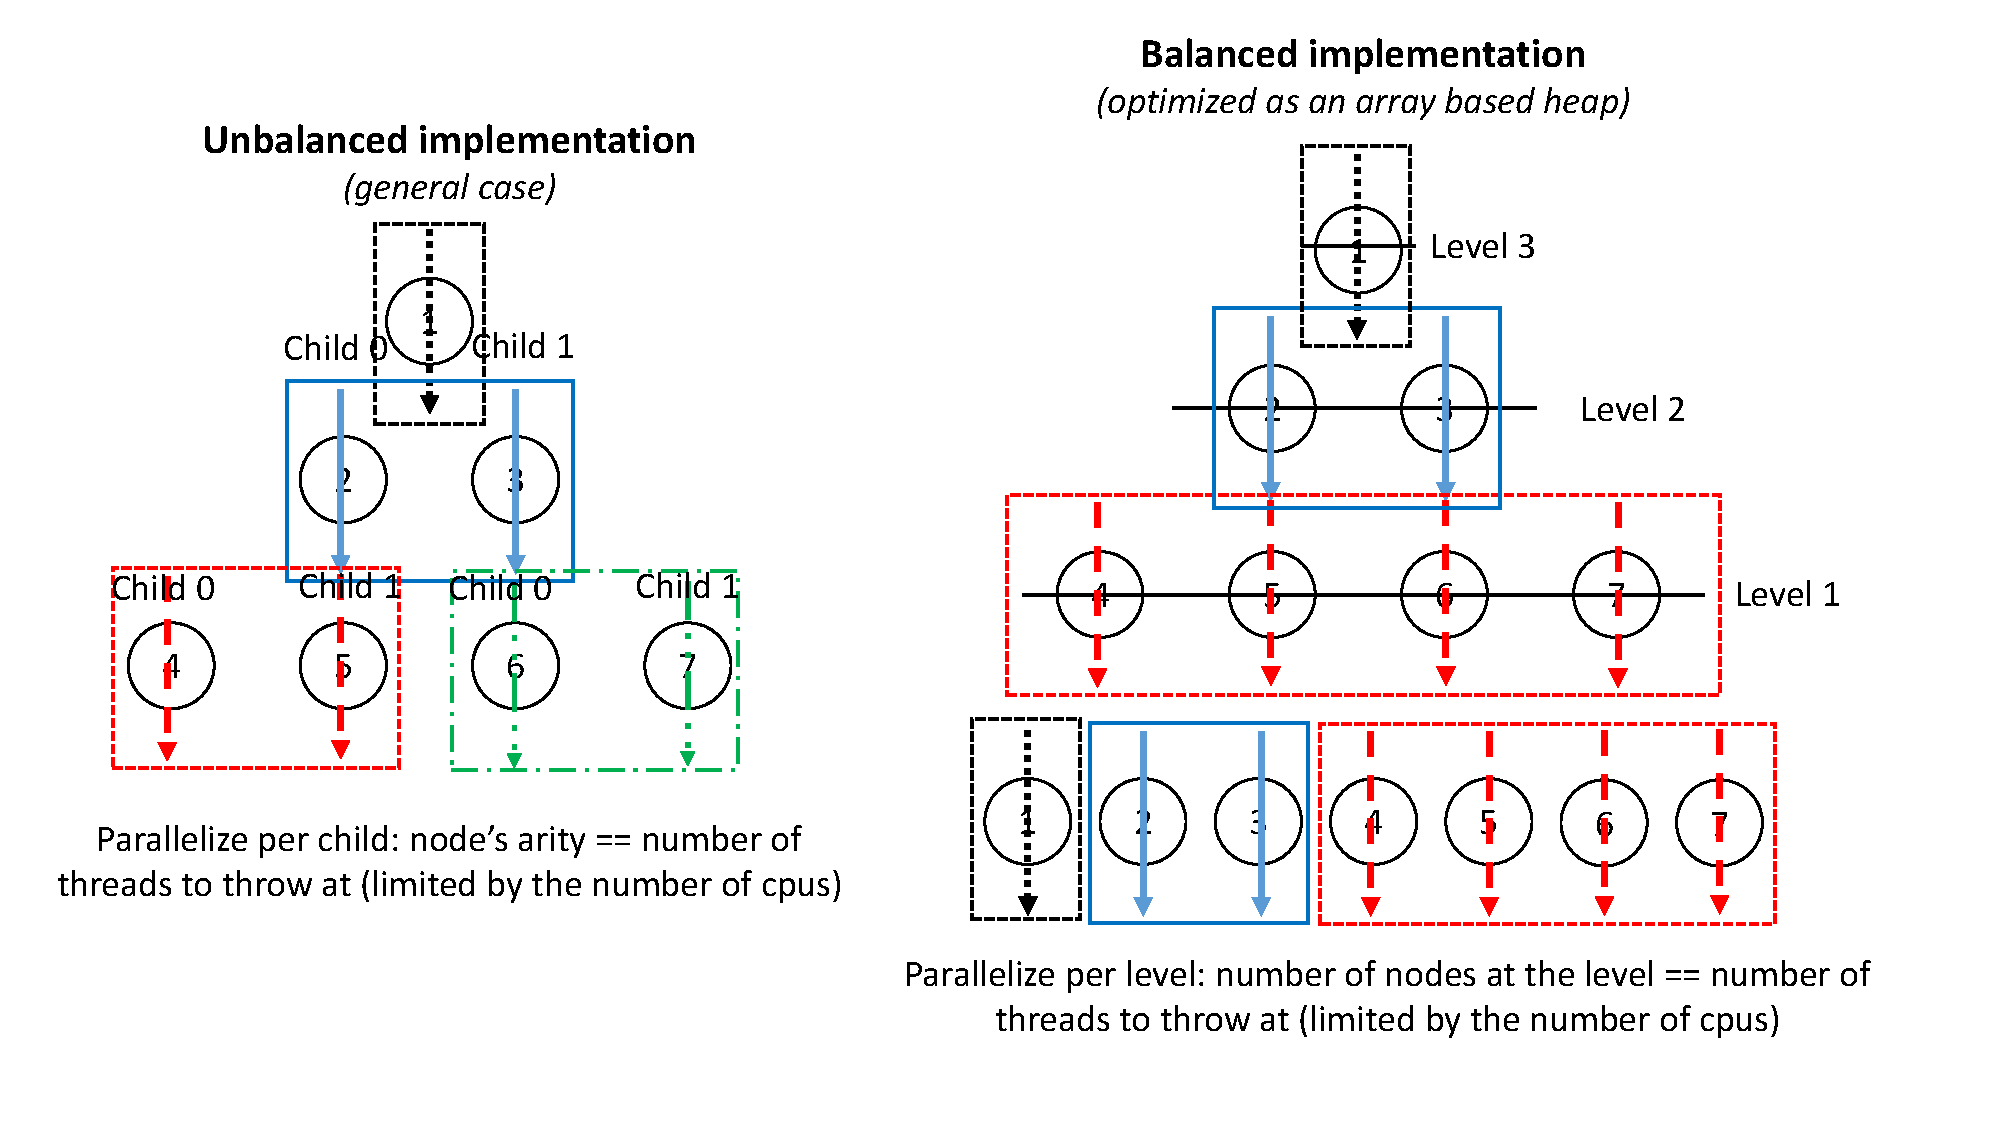
\includegraphics[width=1.0\textwidth]{images/balanced_vs_unbalanced.pdf}
\caption{\textit{Balanced} vs. \textit{Unbalanced} implementations of the fractal framework. Unbalanced implementation handles arbitrary trees and thus is based on pointers. Balanced implementation optimizes the case of a perfect tree and can be implemented with an array.}
\label{fig:balanced_vs_unbalanced}
\end{figure}\newline\null
\quad Figure \ref{fig:performance_health} demonstrates performance of various versions of the \textit{health} benchmark. The benchmark was described in Section \ref{background_benchmarks_olden}. The benchmark grows a tree of hospitals and performs a simulation of the Columbian healthcare system step by step. The number of simulation steps done is plotted on the horizontal axis. The time a simulation took is plotted on a vertical axis. Nodes of the tree, which represent hospitals grow various lists of patients. As simulation goes the lists grow and the nodes become heavier. In other words, the state of the benchmark becomes bigger. The latter has an accumulating effect and contributes to the workload. We can see this phenomenon reflected in an exponential time growth of the sequential version. Parallel versions diminish this time by tackling the task with several threads. This results into 5-6x speedups of the parallel versions relative to sequential ones. This benchmark is an ideal one to tackle with our fractal framework. And indeed, as Figure \ref{fig:performance_health} shows, the thick lines representing the real time (wall clock time) indicate that a parallel versions consistently outperform sequential versions. The sequential versions of our library perform roughly as well as the original legacy C implementation (thin lines vs. a thick \textit{original} line). The latter shows that our library does not introduce any overheads on a benchmark with a significant workload. Dotted lines show the CPU time and illustrate how much of the CPU time has been used by several computational threads of the application. This measure can be used to judge on the aggressiveness of parallelization. 
\begin{figure}[!htb]
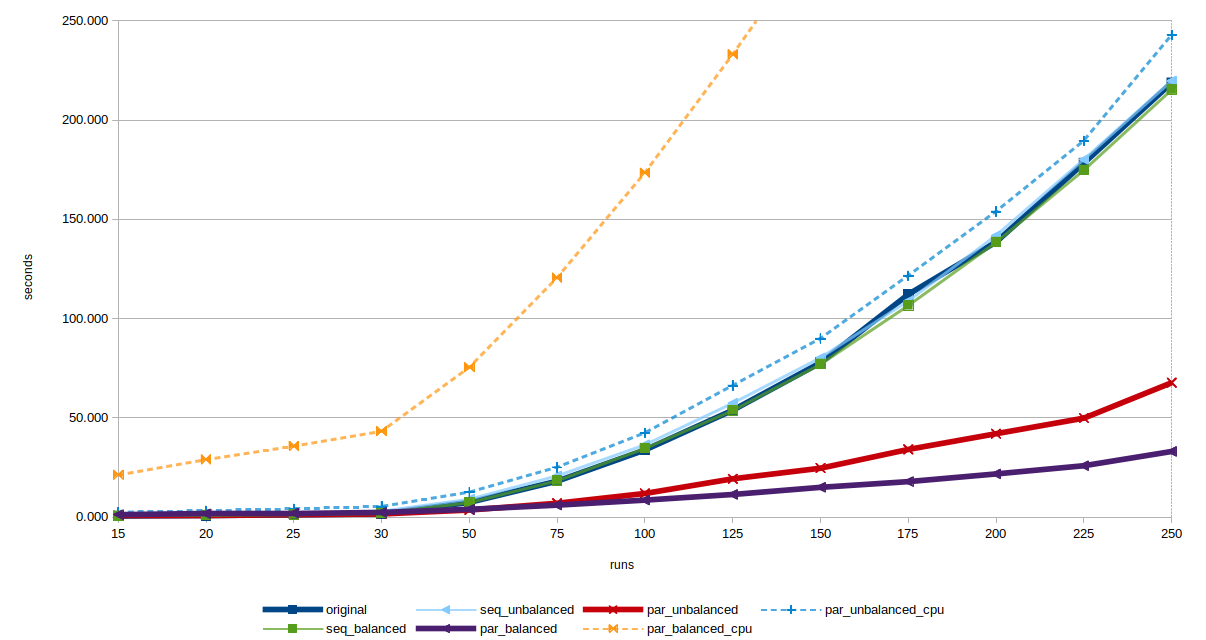
\includegraphics[width=1.0\textwidth]{images/health_depth_10.png}
\caption{Library performance on the \textit{health} benchmark. The legacy C implementation is represented by a thick \textit{original} line. Implementations of the benchmark based on our library are represented by 2 thick (\textit{parallel balanced} and \textit{unbalanced}) and 2 thin (\textit{sequential balanced} and \textit{unbalanced}) lines. Dotted lines represent the CPU time, which is not the real time and has a secondary importance. CPU time reflects the computational workload as we throw several threads at a task and can be used to judge on parallelization aggressiveness.}
\label{fig:performance_health}
\end{figure}\newline\null
\quad Figure \ref{fig:performance_power_reduction_width} illustrates the results for the \textit{power} benchmark. The benchmark performs a workload of scientific computations. The pattern is basically a reduction of folds of folds of reductions. So, the benchmark tests our \textbf{Fold} and \textbf{Reduce} frameworks. We can vary the width of reductions as well as the depth of folds to get various amounts of workload. The benchmark runs repeatedly until the computation result falls withing the set epsilon error. Figure \ref{fig:performance_power_reduction_width} illustrates how the running time of the benchmark scales with an increasing top level reduction width. The latter increases the workload and one can see the growing running time of the sequential original legacy C version. The sequential version based on our library runs roughly as well as the original one, while the parallel version consistently outperforms both sequential versions. Dotted line again represents the CPU time and not the real time. CPU time approximately reflects how many threads were used to run the benchmark. As a validation, one can see that CPU time divided by parallel wall clock time roughly corresponds to the reduction width. Behaviour of the \textit{power} benchmark does not change significantly, when we vary reduction widths or fold depths. We do not include the other experiments we ran, as they do not change the picture.
\begin{figure}[!htb]
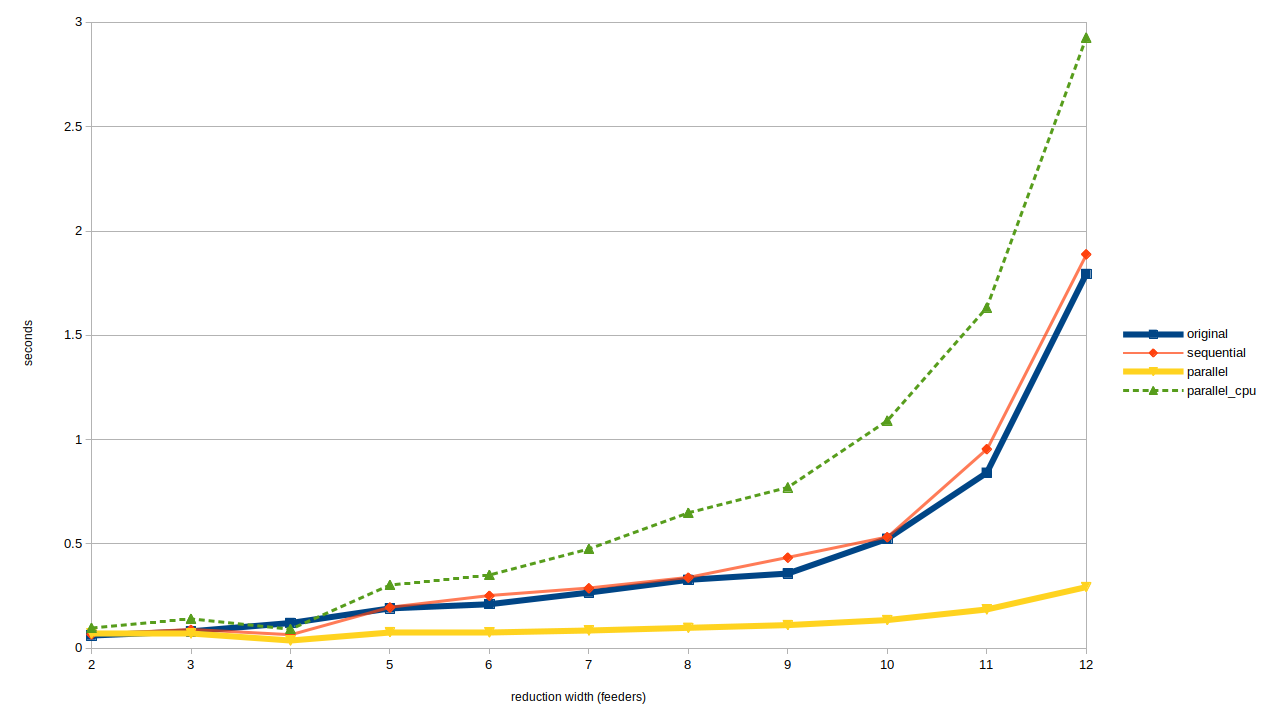
\includegraphics[width=1.0\textwidth]{images/power_reduction_width.png}
\caption{Library performance on the \textit{power} benchmark. We vary the top level (feeders) reduction width to scale the workload.}
\label{fig:performance_power_reduction_width}
\end{figure}\newline\null
\quad The \textit{health} and the \textit{power} benchmarks show the strengths of our library. The \textit{treeadd} and \textit{perimeter} benchmarks highlight its weaknesses. The weaknesses stress the research prototype nature of the library and show places for further optimization effort. Figure \ref{fig:performance_treeadd} shows the behaviour of the \textit{treeadd} benchmark. This benchmark grows a tree with values at its nodes. Then it runs iteratively computing the reduction over the tree and updating node values. The computation is very lighweight. Basically it is just one addition per node processing. The state is minimal and does not accumulate as we run the benchmark over and over. One can see a roughly linear running time of the original legacy C version. Overheads of our sequential library versions are striking for such a small benchmark. Although the asymptotic complexity of all shown versions is the same, various bookkeeping overheads of the library diminish performance relative to the original version with just a single addition per node as the workload. These overheads can be optimized away with some engineering effort, but present in the research prototype library. The more threads we throw the bigger our overheads become. One can see it looking at the running time of balanced and unbalanced versions. It is worthless to tackle such a small benchmark with our library.      
\begin{figure}[!htb]
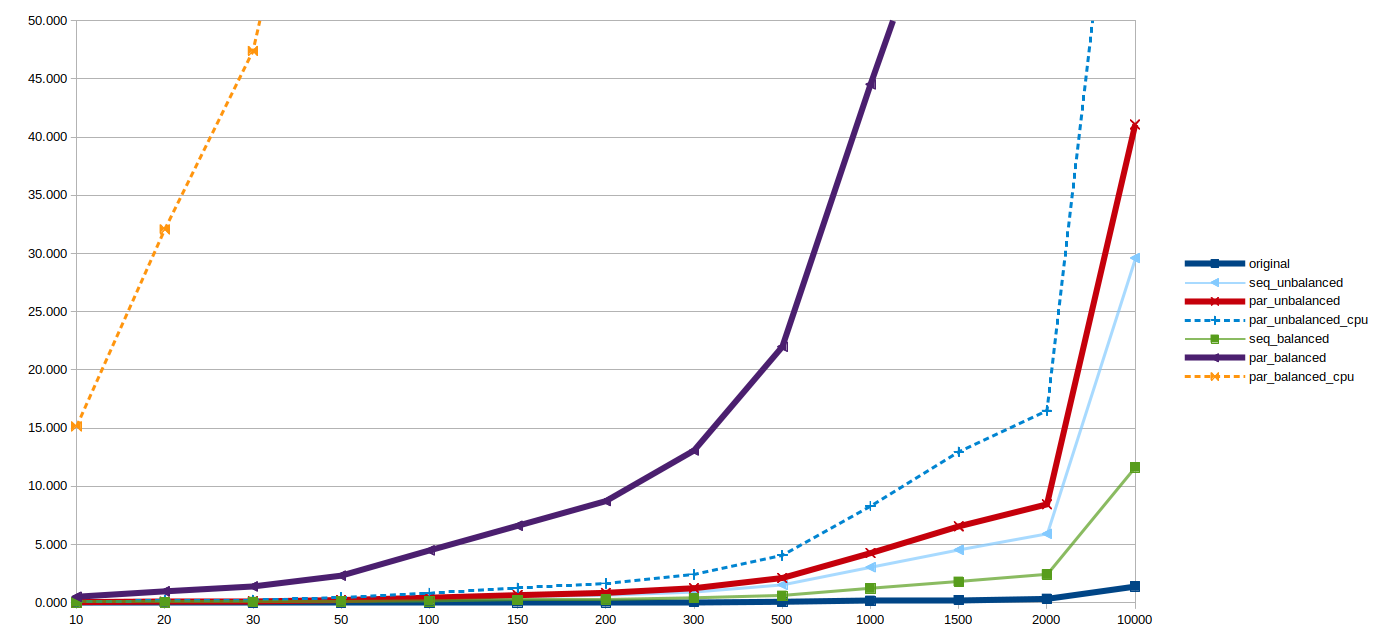
\includegraphics[width=1.0\textwidth]{images/treeadd_depth_16.png}
\caption{Library performance on the \textit{treeadd} benchmark.}
\label{fig:performance_treeadd}
\end{figure}\newline\null
\quad The \textit{perimeter} benchmark shows a different picture, but still highlights the current weaknesses of the library implementation. Figure \ref{fig:performance_perimeter} shows the bar chart. The benchmark does not run an iterative simulation as the 3 other benchmarks do - it is a single perimeter computation. Horizontal axis plots the depth of the tree underlying perimeter computation, a workload size in other words. As usual, the vertical axis plots the time it took to run the computation. As the benchmark is based on an unbalanced tree version we cannot run it with a balanced implementation. Here we have only the original sequential legacy C implementation, the sequential implementation based on our library and its parallel counterpart. One can see that the benchmark also highlights the current implementation problems: original does better than sequential. At the same time the benchmark has a potential: there is a good parallel speedup when we compare the sequential versus parallel library based versions.
\begin{figure}[!htb]
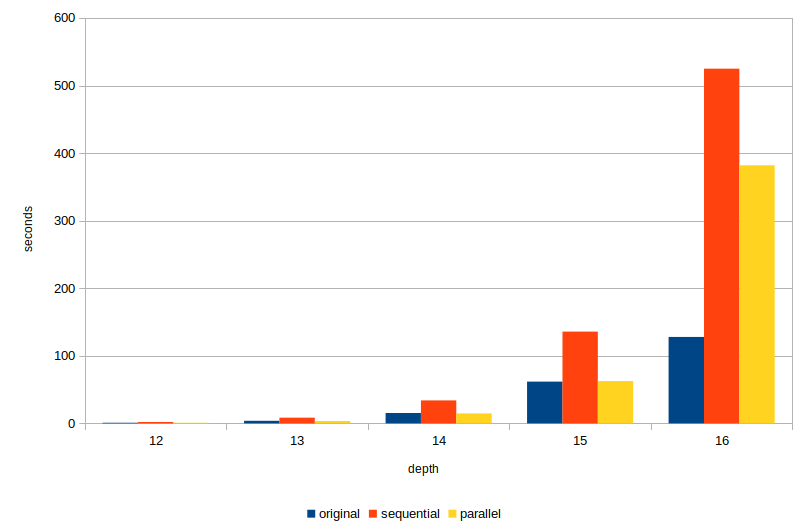
\includegraphics[width=1.0\textwidth]{images/perimeter.png}
\caption{Library performance on the \textit{perimeter} benchmark. Horizontal axis plots the depth of the perimeter tree (see Section \ref{background_benchmarks_olden}). Vertical axis shows the time it takes to compute a single perimeter value with various tree depths (splitting granularity).}
\label{fig:performance_perimeter}
\end{figure}

\section{Limitations and Future work}
\label{frameworks_future_work}
\subsection{Limitations}
\label{frameworks_limitations}
\quad The limitations of our computational frameworks largely come as the implications of unconstrained allowance of side effects. Compared to pure functional patterns our computational frameworks give a programmer more freedom by allowing to leave side effects, but this comes at the price of programmers having more responsibility. It is an interesting trade-off by itself, but a programmer still needs to understand computational patterns our frameworks support and a high-level parallelization they do to prevent possible race conditions. Aside conforming to a certain interface, our computational frameworks do not impose any particular restrictions on operator functions and provide a programmer with a freedom. Obviously, our computational frameworks are not universal and are limited to only those problems they are applicable to.
\subsection{Future work}
\label{frameworks_fw}
\quad Chapter \ref{related_work} presents an overview of related work on various automatic and semi-automatic software parallelization methods. Automatically parallelizing compilers are challenged by the limitations of static program analysis. As a workaround solution, various researchers have proposed techniques on automatic data structure and algorithmic skeleton recognition. The application of these techniques for the real world code could be exacerbated by the problem of algorithm and data structure inseparability.\newline\null
\quad The concept of computational frameworks and the prototype library could lay the foundation towards an alternative automatic parallelization technique. We believe that it is possible to automatically recognize computational frameworks in the suite of Olden benchmarks. Alike the work \cite{skeletons-static}, the recognition technology could be based on the static analysis of the program's AST. Figure \ref{fig:parallelization_scheme} shows the scheme. It takes an original legacy C source code, where we supposedly have a computation that fits into one or several of our frameworks. The task of the recognizer is to identify a computational pattern. Like in the case of the \textit{health} Olden benchmark we have a recursive \textit{grow()} and \textit{compute()} procedures, which build and process the tree correspondingly. That recursive pattern can be matched to a fractal framework. The next step would be to strip the code corresponding and implementing the pattern (\textit{backbone logic}) and leave the rest as the \textit{business logic}. The business logic must be further classified into various computational framework template class methods (like \textit{grow()}, \textit{growth\_stop\_condition()}, \textit{inject()}, etc.). Then, the class template must be instantiated with the business logic inserted into the right places. Once that is done, the parallelization is done, as the compiler will take care of everything else.
\begin{figure}[!htb]
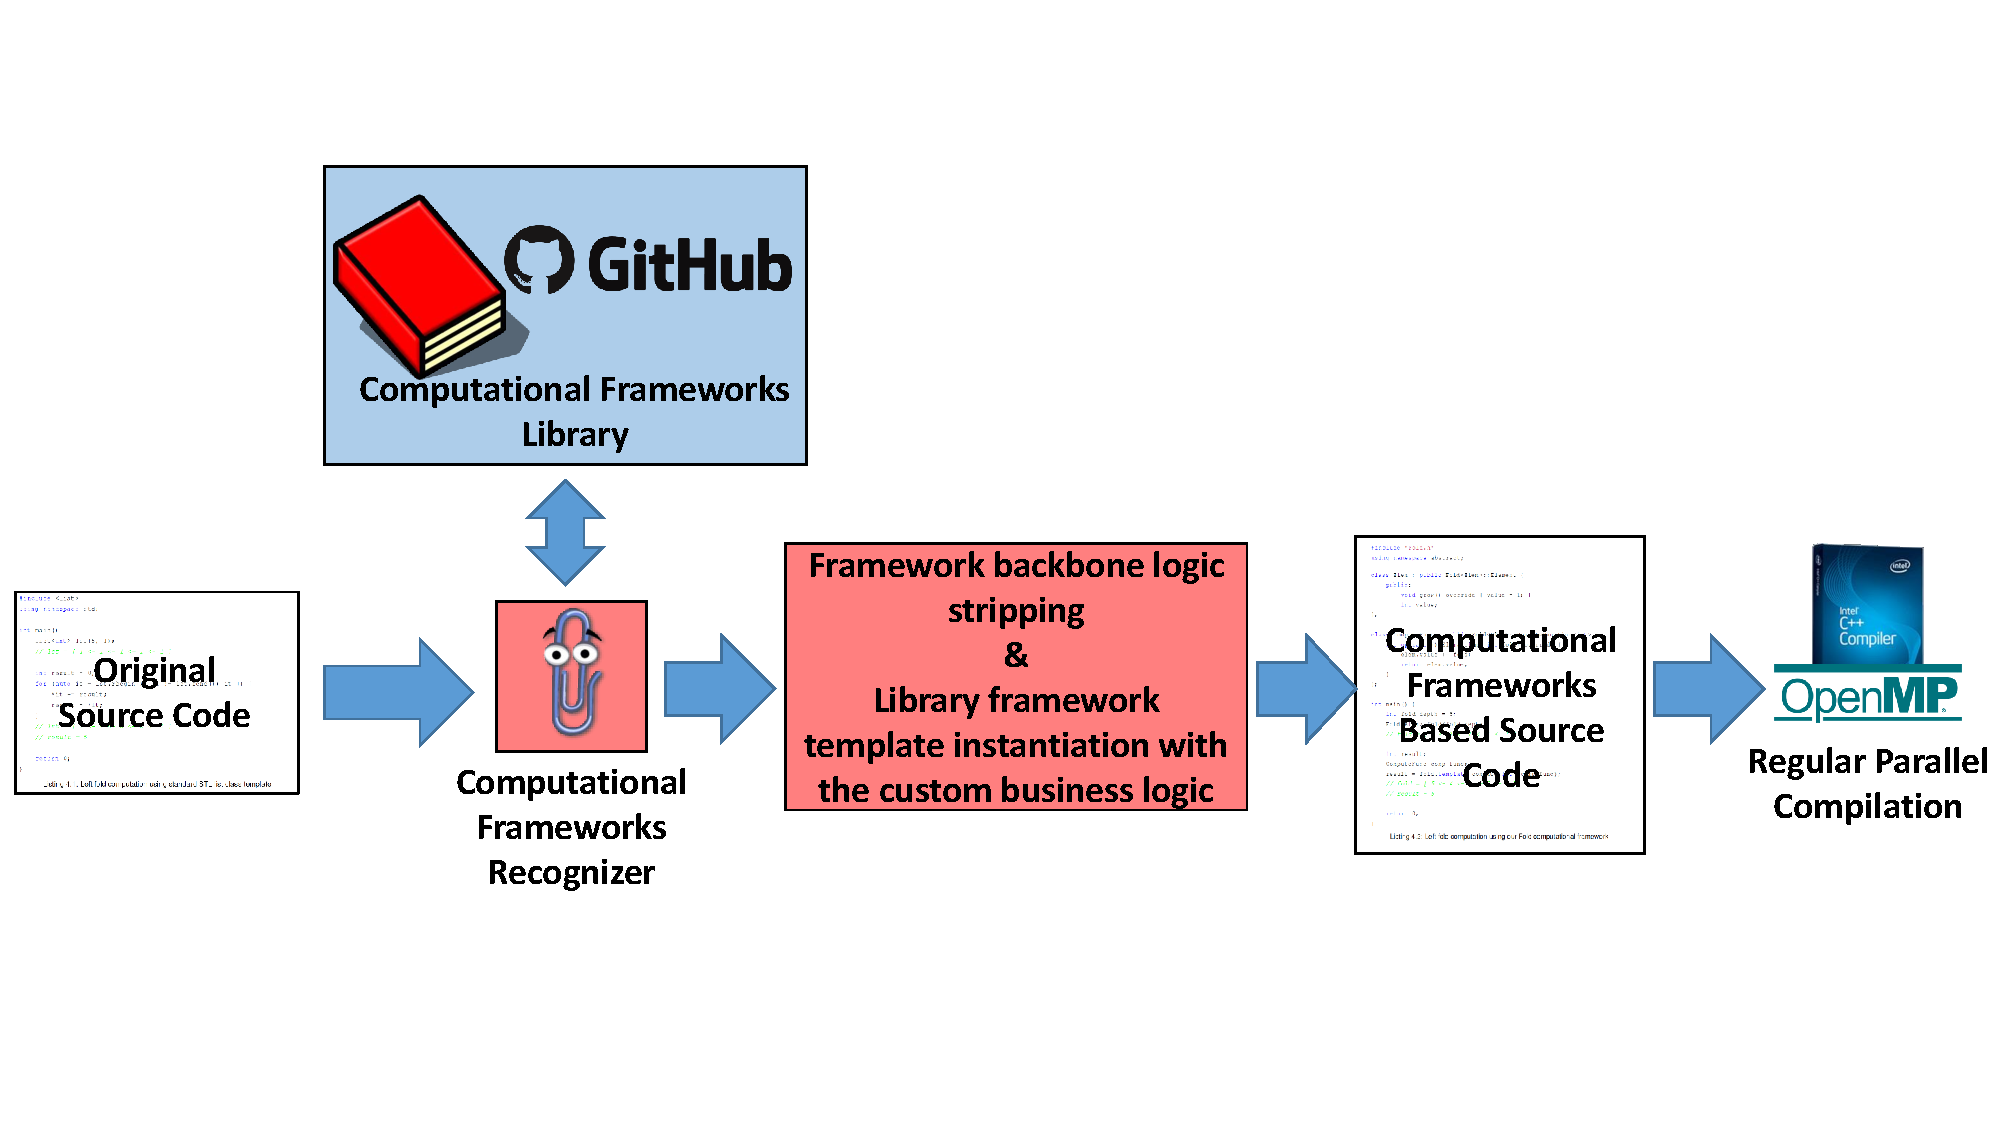
\includegraphics[width=1.0\textwidth]{images/parallelization_scheme.pdf}
\caption{An alternative software parallelization scheme based on our library of computational frameworks.}
\label{fig:parallelization_scheme}
\end{figure}\newline\null
\quad Technically, for benchmarks as simple as Olden the technique can work on the level of the compiler's front end: source code or an abstract syntax tree (AST). That sets the technique apart from the regular parallelization approaches based on dependence graphs and working on the level of the compiler's intermediate representation (IR). For more complex applications dynamic trace-based techniques could be used.\newline\null
\quad We envision this work as a possible future direction.

%%

\chapter{Summary \& Conclusions}
\label{conclusion}
\quad Parallelism has become pervasive in the modern computing world. Parallel hardware is everywhere, but to exploit the available resources software has to be effectively mapped onto that hardware. The areas of \textit{software parallelization} and \textit{parallel software development} are extremely important. Despite decades of academic research and industrial investment into the area, the human expert still has a major role to play. Our state-of-the-art literature review shows that there are still no automatic solutions that could fully replace an expert programmer and at the same time guarantee program correctness and achieve performance results comparable to those of manually parallelized software.\newline\null
\quad In order to achieve the best result a programmer has to work on multiple conceptual levels starting from problem decomposition and algorithm choice down to low level loop transformations. In this thesis we fully acknowledge the role of the human expert, but provide the latter with an \textit{assistant solution}, which aims at alleviating the software parallelization and parallel software development tasks. The solution is as multifaceted as the problem itself, and also spans several conceptual levels. It consists of the two components: a tool plus methodology and a library of parallel primitives. The tool aims to alleviate the task of sequential software parallelization by guiding a programmer through the process. The library can be used as a set of ready solutions for specific problems to develop parallel software from scratch.\newline\null
\quad The tool aims to assist human experts by guiding them directly towards the most interesting program loops from the perspective of software parallelization, thus alleviating the parallelizable code search process and delivering savings for this costly human resource. We have developed a novel machine learning based approach to predicting whether or not a loop is parallelizable. We combine this prediction with traditional profiling information and develop a ranking function that prioritizes low-risk, high-gain loop candidates, which are finally presented to the user.\newline\null
\quad We have evaluated our parallelization assistant against the sequential C implementations of the SNU NPB suite. We show that our assistant recognizes parallelizable loops more aggressively than conservative parallelizing compilers, thus improving parallelism discovery. We also show that our parallelization assistant can increase programmer productivity. Our experiments confirm, that equipped with our assistant, a programmer is required to examine and parallelize substantially fewer loops to achieve performance levels comparable to those of the reference OpenMP implementations of the benchmarks.\newline\null
\quad Our work has demonstrated that there is scope for machine learning based tool support in parallelization despite its inherent lack of safety. By assisting human programmers rather than replacing them, machine learning techniques have the potential to deliver productivity gains beyond what is possible by relying on traditional parallelization approaches alone.\newline\null
\quad The second component of the assistant solution is the concept of \textit{computational frameworks} along with a research prototype library implementing it. In our benchmark feasibility studies we show that the problem of successful data structure choice stands particularly important and can vastly affect the parallelizability of programs. Moreover, we observe \textit{the problem of algorithm and data structure inseparability}. These issues has led us to a novel concept of computational frameworks, which are higher level entities that embody algorithms and data structures together into an elegant and well-structured construct. Computational frameworks can be used as parallel software design and construction primitives alleviating the task and ultimately parallelizing a wide class of applications, which fit into their computational patterns.\newline\null
\quad We shaped the concept and designed the library using a subset of the Olden benchmarks. We expressed benchmark computations through our \textit{Fractal}, \textit{Fold} and \textit{Reduce} frameworks and rewrote the benchmarks in a modern, well-structured and crucially parallel way combining the elements of both object-oriented and functional programming. Moreover, the rejuvenated C++ benchmark versions demonstrate a good parallel performance compared to their serial legacy C counterparts. On the major benchmarks we achieve 5-6x speedups. However, given the research prototype nature of the library, some further engineering effort is still needed.\newline\null
\quad In this thesis we demonstrate that when decades old and well-known methods of software parallelization such as various automatic techniques run into their limits and fail to tackle the challenges of the real world codes, and more exotic methods of machine learning based techniques run into their principal problems of inherent statistical errors and the lack of safety, it is possible to acknowledge the role of a human expert and resort to various assisting solutions. The latter demonstrate promising results and pave an attractive future research direction.

%

%%%%%%%%
%% Any appendices should go here. The appendix files should look just like the
%% chapter files.
\appendix
\include{appendix1}
%% ... etc...

%% Choose your favourite bibliography style here.
\bibliographystyle{apalike}

%% If you want the bibliography single-spaced (which is allowed), uncomment
%% the next line.
% \singlespace

%% Specify the bibliography file. Default is thesis.bib.
%\bibliography{main.bib}

\printbibliography

%% ... that's all, folks!
\end{document}
